\documentclass[journal]{new-aiaa}
%\documentclass[conf]{new-aiaa} for conference papers
\usepackage{AAS_packages}
% \usepackage[utf8]{inputenc}

% \usepackage[version=4]{mhchem}
% \usepackage{longtable,tabularx}
% \setlength\LTleft{0pt} 

\title{Real Time Adaptive Shape Reconstruction for Asteroid Landing}

\author{Shankar Kulumani \footnote{PhD, Mechanical and Aerospace Engineering, \href{skulumani@gwu.edu}{mailto:skulumani@gwu.edu}}
and
Taeyoung Lee \footnote{Associate Professor, Mechanical and Aerospace Engineering, \href{tylee@gwu.edu}{mailto:tylee@gwu.edu}}}
\affil{Goerge Washington University, Washington, DC, 20052}

\begin{document}

\maketitle

\begin{abstract}
    Knowledge of the shape of an asteroid is crucial for spacecraft operations.
    The standard method of determining the gravitational potential, through the use of a polyhedron potential model, is dependent on the shape model.
    Furthermore, accurate landing or low altitude operations requires accurate knowledge of the surface topology. 
    The typical approach to shape determination requires an extensive ``mapping'' phase of the mission over which extensive measurements are collected and transmitted for Earth-based processing.
    Instead, we present an efficient method for estimating the shape of an asteroid in real time.
    Range measurements of the surface are used to incrementally correct an initial shape estimate according to Bayesian framework. 
    Then, an optimal guidance scheme is proposed to control the vantage point of the range sensor to construct a more accurate model of the asteroid shape. 
    This shape model is then used in a nonlinear controller to track a desired trajectory about the asteroid.
    % Finally, a multi resolution approach is presented which enables for a higher fidelity shape representation in a specified location while avoiding the inherent burdens of a uniformly high resolution mesh. 
    This approach enables for an accurate shape determination around a potential landing site.
    We demonstrate this approach using several radar shape models of asteroids and provide a full dynamic simulation about asteroid 4769 Castalia.
\end{abstract}

\section*{Nomenclature}

\noindent(Nomenclature entries should have the units identified)

% {\renewcommand\arraystretch{1.0}
% \noindent\begin{longtable*}{@{}l @{\quad=\quad} l@{}}
% $A$  & amplitude of oscillation \\
% $a$ &    cylinder diameter \\
% $C_p$& pressure coefficient \\
% $Cx$ & force coefficient in the \textit{x} direction \\
% $Cy$ & force coefficient in the \textit{y} direction \\
% c   & chord \\
% d$t$ & time step \\
% $Fx$ & $X$ component of the resultant pressure force acting on the vehicle \\
% $Fy$ & $Y$ component of the resultant pressure force acting on the vehicle \\
% $f, g$   & generic functions \\
% $h$  & height \\
% $i$  & time index during navigation \\
% $j$  & waypoint index \\
% $K$  & trailing-edge (TE) nondimensional angular deflection rate\\
% $\Theta$ & boundary-layer momentum thickness\\
% $\rho$ & density\\
% \multicolumn{2}{@{}l}{Subscripts}\\
% cg & center of gravity\\
% $G$ & generator body\\
% iso	& waypoint index
% \end{longtable*}}




\section{Introduction}
% Motivation for missions/studying asteroids
Small solar system bodies, such as asteroids and comets, continue to remain a focus of scientific study.
The small size of these bodies prevents the formation of large internal pressures and temperatures which helps to preserve the early chemistry of the solar system.
This insight offers additional detail into the formation of the Earth and also of the probable formation of other extrasolar planetary bodies.
Of particular interest are those near-Earth asteroids (NEA) which inhabit heliocentric orbits in the vicinity of the Earth. 
These easily accessible bodies provide attractive targets to support space industrialization, mining operations, and scientific missions.
In spite of the significant interest, and the extensive research by the community, the operation of spacecraft near small bodies remains a challenging problem.

% dynamics are difficult around asteroids
The dynamic environment around asteroids is strongly perturbed and challenging for analysis and mission operations~\cite{scheeres2012}.
Due to their low mass, which in turn causes a low gravitational attraction, asteroids may have irregular shapes.
Furthermore, asteroids may also have a chaotic spin state due to the absorption and emittance of solar radiation~\cite{rubincam2000}.
As a result, approaches utilizing an inverse square gravitational model do not capture the  true dynamic environment.
In addition, the vast majority of asteroids are difficult to track and characterize using ground based sensors.
Due to their small size, frequently with a maximum radius less than \SI{1}{\kilo\meter}, and low albedo, the reflected energy of these asteroids is insufficient for reliable detection or tracking.
Therefore, the dynamics model of the asteroid is relatively coarse prior to in situ measurements from a dedicated spacecraft.
As a result, any spacecraft mission to an asteroid must include the ability to update the dynamic model given in situ measurements and remain robust to unmodelled forces.

Another key dynamic consideration is the coupling between rotational and translational states around the asteroid.
The coupling is induced due to the different gravitational forces experienced on various portions of the spacecraft. 
The effect of the gravitational coupling is related to the ratio of the spacecraft size and orbital radius~\cite{hughes2004}.
For operations around asteroids, the ratio is relatively large which causes a much larger coupling between the translational and rotational states.
References~\citenum{elmasri2005} and~\citenum{sanyal2004a} investigated the coupling of an elastic dumbbell spacecraft in orbit about a central body, but only considered the case of a spherically symmetric central body.
Furthermore, the spacecraft model is assumed to remain in a planar orbit.
As a result, these developments are not directly applicable to motion about an asteroid, which experiences highly non-Keplerian motion.
Reference~\citenum{misra2015b} investigated the effect of coupled motion on long term trajectories around asteroids.
However, the analysis only considered a second order spherical harmonic gravitational potential model. 
Therefore, these results are only valid when far from the asteroid surface and will diverge when used within the Brillouin sphere.

% Gravity model is important and dependent on shape
An accurate gravitational potential model is critical for performing low altitude and/or surface operations around asteroids.
Due to the irregular shape, trajectories will pass within the Brillouin sphere, where the typical spherical harmonic model diverges from the true gravitational potential.
The standard approach for asteroid missions is to compute the gravitational potential using a polyhedron potential model~\cite{werner1996}.
The polyhedron potential model provides the exact gravitational potential, and subsequently the gravitational acceleration, for a given triangular faceted shape model of an asteroid.
The method provides the exact potential at any point outside the body for a given shape model.
As a result, the accuracy of the gravitational potential is primarily dependent on the accuracy with which the shape model represents the true surface.
A high fidelity shape, which necessarily has many vertices and faces, is required for an accurate computation of the gravitational acceleration and enabling low altitude operations.

% Challenges involved in operation near asteroids (gravity, shape, distance)
% generating the shape from the ground is difficult
Prior to the arrival of a spacecraft at an asteroid, Earth-based sensors are used to characterize the body.
Using both optical and radar sensors allows for the precise orbit of the asteroid to be determined.
Another vital task is the determination of the asteroid shape from radar data~\cite{hudson1994,busch2011}.
This is a challenging problem as it requires the simultaneous estimation of the asteroid spin state and shape.
Furthermore, determining the shape from radar is currently the only Earth-based technique that can produce detailed three-dimensional shape information of near-Earth objects~\cite{greenberg2015}.
The current approach is based on an estimation scheme which iteratively perturbs a shape to match given radar data.
This computationally intensive approach is only able to capture the gross size and shape and is unable to capture the small surface features of the asteroid.
Frequently, only a coarse model is possible from the ground and an accurate shape must be determined only after a spacecraft has rendezvoused with the asteroid.
As a result, upon arrival the gravitational environment near the asteroid is poorly modeled as the shape of the asteroid is not accurate.
Therefore, the polyhedron potential model is not appropriate immediately upon arrival but rather only after the shape has been determined.

% on arrival spacecraft spend long periods mapping, and depending on mission this might be unallocable
On approach to an asteroid, spacecraft navigation and guidance is primarily based on ground measurements.
After arrival, a spacecraft will generally spend months or years in a mapping mission phase~\cite{kubota2003,cole1998}.
During this period, spacecraft sensors, such as on board optical telescopes or Light radio Detection and Ranging (LIDAR), are used to characterize the asteroid.
The resulting imagery and range data is transmitted to the ground and the resulting asteroid shape and motion is estimated. 
During this mapping phase the spacecraft must remain in a quiescent state devoted entirely to mapping the surface.
Depending on the mission type, this long period of mapping is crucial to the mission, such as sample collection~\cite{gates2015}. 
However, other missions, such as asteroid mitigation, may be severely limited by the time and ground resources required to generate a surface shape.
Furthermore, the long distances involved necessitate on-board autonomy to enable to spacecraft to operate without ground communications.
Similarly, during landing the spacecraft will require the ability to sense and model the surface topography in order to safely land in an unknown environment.
The dependency on expensive ground-based shape reconstruction techniques limits the ability of spacecraft to autonomously operate at asteroids.
Mitigation of this ground based surface modeling will greatly expand the range of missions possible.

% we want to generate the shape in real time and then use this shape for updated and better control
In this paper, we develop a method to compute the surface shape of an asteroid from range measurements.
Our approach is able to operate in real time and incrementally update the shape model of an asteroid as new range measurements are collected.
This approach allows for the shape to be continually updated as range measurements are used to locally modify the shape estimate.
Furthermore, this updated shape is then used in a nonlinear controller to enable the tracking of a landing trajectory to the surface.
In contrast to previous work, we explicitly consider the gravitational coupling between orbit and attitude dynamics.
Furthermore, instead of computationally expensive surface reconstruction methods, we present a straightforward and conceptually simple method to enable real time shape updates. 


% our approach for paper. Real time method to update asteroid shape model and use updated model in closed loop control

% Benefits and contribution of our approach
In short, this paper presents a method to incrementally update the shape  model of an asteroid from range measurements. 
Our approach alleviates the need for a dedicated mapping phase as the spacecraft is able to update its shape model in real time and without expensive computations.
This type of approach allows for the spacecraft to maneuver and land on the asteroid immediately upon arrival rather than spending several months mapping the surface.
This updated shape model is then used to in a nonlinear controller to track a desired state trajectory for the dynamics of a rigid body spacecraft.
The dynamics are developed on the nonlinear manifold of rigid body motions, namely the special euclidean group.
This formulation is based on an intrinsic geometric description of the motion and accurately captures the coupling between orbit and attitude dynamics. 
The presented approach allows for a spacecraft to transition directly from arrival to the surface while reconstructing the surface shape in real time.

\section{Problem Formulation}\label{sec:problem}

In this paper, we consider the motion of a dumbbell model of spacecraft around an asteroid.
The dumbbell model captures the important interactions of the coupling between orbital and attitude dynamics.
In this model, the spacecraft consists of two masses connected by a massless rod.
The asteroid is modeled as a constant density polyhedron with constant, and known, spin about its maximum moment of inertia. 
Without loss of generality, we define body fixed frames for both the spacecraft and asteroid, which are aligned with the principle axes of each body and originate at their respective center of mass. 
The kinematics of the dumbbell and asteroid are described in the inertial frame by
\begin{itemize}
    \item \( \vc{x} \) - the position of the center of mass of the dumbbell spacecraft represented in the inertial frame, \( \vc{e}_i\),
    \item \( R \) - the rotation matrix which transforms vectors defined in the spacecraft fixed frame, \( \vc{b}_i \), to the inertial frame, \( \vc{e}_i \),
    \item \( \vc{\Omega} \) - the angular velocity of the spacecraft body fixed frame relative to the inertial frame and represented in the dumbbell body fixed frame, \( \vc{b}_i \), and
    \item \( R_A \) - the rotation matrix which transforms vectors defined in the asteroid fixed frame, \( \vc{f}_i \), to the inertial frame, \( \vc{e}_i \).
\end{itemize}
In this work, we assume that the asteroid is much more massive than the spacecraft and its motion is not affected by that of the spacecraft.
This assumption allows us to treat the motion of the vehicle independently from that of the asteroid. 

\subsection{Spacecraft Dynamic Model}
Using Hamilton's principle one can derive the inertial equations of motion of the dumbbell spacecraft~\cite{kulumani2017b} as
\begin{align}
    \dot{\vc{x}} &= \vc{v}, \\
    \parenth{m_1 + m_2} \dot{\vc{v}} &= m_1 R_A \deriv{U}{\vc{z}_1} + m_2 R_A \deriv{U}{\vc{z}_2}, \\
    \dot{R} &= R S(\vc{\Omega}) , \\
    J \dot{\vc{\Omega}} + \vc{\Omega} \times J \vc{\Omega} &= \vc{M}_1 + \vc{M}_2.
\end{align}
The vectors \( \vc{z}_1 \) and \( \vc{z}_2\) define the position of the dumbbell masses in the asteroid fixed frame and are defined as
\begin{align}
    \vc{z}_1 &= R_A^T \parenth{\vc{x} + R \vc{\rho}_1} , \\
    \vc{z}_2 &= R_A^T \parenth{\vc{x} + R \vc{\rho}_2}.
\end{align}
The gravitational moment on the dumbbell \( \vc{M}_i\) is defined as
\begin{align}
    \vc{M}_i = m_i \parenth{S(R_A^T \vc{\rho}_i) R^T \deriv{U}{\vb{z}_i}}.
\end{align}
where the polyhedron potential is defined as 
\begin{align}
    U(\vc{r}) &= \frac{1}{2} G \sigma \sum_{e \in \text{edges}} \vc{r}_e \cdot \vc{E}_e \cdot \vc{r}_e \cdot L_e - \frac{1}{2}G \sigma \sum_{f \in \text{faces}} \vc{r}_f \cdot \vc{F}_f \cdot \vc{r}_f \cdot \omega_f,
\end{align}
and \( \vc{r}_e\) and \(\vc{r}_f \) are the vectors from the spacecraft to any point on the respective edge or face, \( G\) is the universal gravitational constant, and \( \sigma \) is the constant density of the asteroid.
The position of each mass \(m_i\) of the dumbbell is defined in the dumbbell fixed frame by the vector \(\vb{\rho}_i\). 


\subsection{Polyhedron Potential Model}\label{sec:polyhedron_potential}

% most use a spherical harmonic model or a ellipsoid model but we use a polyhedron model
An accurate gravitational potential model is necessary for the operation of spacecraft about asteroids.
Additionally, a detailed shape model of the asteroid is needed for trajectories passing close to the body.
The classic approach is to expand the gravitational potential into a harmonic series and compute the series coefficients.
However, the harmonic expansion is always an approximation as a result of the infinite order series used in the representation.
Additionally, the harmonic model used outside of the circumscribing sphere is not guaranteed to converge inside the sphere, which makes it unsuitable for trajectories near the surface.

We represent the gravitational potential of the asteroid using a polyhedron gravitation model.
This model is composed of a polyhedron, which is a three-dimensional solid body, that is defined by a series of vectors in the body-fixed frame.
The vectors define vertices in the body-fixed frame as well as planar faces which compose the surface of the asteroid.
We assume that each face is a triangle composed of three vertices and three edges.
As a result, only two faces meet at each edge while three faces meet at each vertex.
Only the body-fixed vectors, and their associated topology, is required to define the exterior gravitational model.
References~\cite{werner1994} and~\cite{werner1996} give a detailed derivation of the polyhedron model.
Here, we summarize the key developments and equations required for implementation.

Consider three vectors \( \vc{v}_1, \vc{v}_2, \vc{v}_3 \in \R^{3 \times 1} \), assumed to be ordered in a counterclockwise direction about an outward facing normal vector, which define a face.
For each face we define the face dyad \( \vc{F}_f \) as
\begin{align}\label{eq:face_dyad}
    \vc{F}_f &= \hat{\vc{n}}_f \hat{\vc{n}}_f \in \R^{3 \times 3}.
\end{align}
Each edge is a member of two faces and has an outward pointing edge normal vector, perpendicular to both the edge and the face normal.
For the edge connecting the vectors \( \vc{v}_1 \) and \( \vc{v}_2 \), which are shared between the faces \(A\) and \( B\), the per edge dyad is given by
\begin{align}\label{eq:edge_dyad}
    \vc{E}_{12} = \hat{\vc{n}}_A \hat{\vc{n}}_{12}^A + \hat{\vc{n}}_B \hat{\vc{n}}_{21}^B \in \R^{3 \times 3}.
\end{align}
The edge dyad \( \vc{E}_e  \), is defined for each edge and is a function of the two adjacent faces meeting at that edge.
The face dyad \( \vc{F}_f \), is defined for each face and is a function of the face normal vectors.

Let \( \vc{r}_i \in \R^{3 \times 1} \) be the vector from the spacecraft to the vertex \( \vc{v}_i \) and it's length is given by \( r_i = \norm{\vc{r}_i} \in \R^{1} \).
The per-edge factor \( L_e \in \R^{1}\), for the edge connecting vertices \( \vc{v}_i \) and \( \vc{v}_j \), with a constant length \( e_{ij} = \norm{\vc{e}_{ij}} \in \R^1\) is
\begin{align}\label{eq:edge_factor}
    L_e &= \ln \frac{r_i + r_j + e_{ij}}{r_i + r_j - e_{ij}}.
\end{align}
For the face defined by the vertices \( \vc{v}_i, \vc{v}_j, \vc{v}_k \) the per-face factor \( \omega_f \in \R^{1} \) is
\begin{align}\label{eq:face_factor}
    \omega_f &= 2 \arctan \frac{\vc{r}_i \cdot \vc{r}_j \times \vc{r}_k}{r_i r_j r_k + r_i \parenth{\vc{r}_j \cdot \vc{r}_k} + r_j \parenth{\vc{r}_k \cdot \vc{r}_i} + r_k \parenth{\vc{r}_i \cdot \vc{r}_j}} .
\end{align}
The gravitational potential due to a constant density polyhedron is given as
\begin{align}\label{eq:potential}
    U(\vc{r}) &= \frac{1}{2} G \sigma \sum_{e \in \text{edges}} \vc{r}_e \cdot \vc{E}_e \cdot \vc{r}_e \cdot L_e - \frac{1}{2}G \sigma \sum_{f \in \text{faces}} \vc{r}_f \cdot \vc{F}_f \cdot \vc{r}_f \cdot \omega_f \in \R^1,
\end{align}
where \( \vc{r}_e\) and \(\vc{r}_f \) are the vectors from the spacecraft to any point on the respective edge or face, \( G\) is the universal gravitational constant, and \( \sigma \) is the constant density of the asteroid.
Furthermore we can use these definitions to define the attraction, gravity gradient matrix, and Laplacian as
\begin{align}
    \nabla U ( \vc{r} ) &= -G \sigma \sum_{e \in \text{edges}} \vc{E}_e \cdot \vc{r}_e \cdot L_e + G \sigma \sum_{f \in \text{faces}} \vc{F}_f \cdot \vc{r}_f \cdot \omega_f \in \R^{3 \times 1} , \label{eq:attraction}\\
    \nabla \nabla U ( \vc{r} ) &= G \sigma \sum_{e \in \text{edges}} \vc{E}_e  \cdot L_e - G \sigma \sum_{f \in \text{faces}} \vc{F}_f \cdot \omega_f \in \R^{3 \times 3}, \label{eq:gradient_matrix}\\
    \nabla^2 U &= -G \sigma \sum_{f \in \text{faces}}  \omega_f \in \R^1 .\label{eq:laplacian}
\end{align}

One interesting thing to note is that both~\cref{eq:face_dyad,eq:edge_dyad} can be precomputed without knowledge of the position of the satellite.
They are both solely functions of the vertices and edges of the polyhedral shape model and are computed once and stored.
Once a position vector \( \vc{r} \) is defined, the scalars given in~\cref{eq:edge_factor,eq:face_factor} can be computed for each face and edge.
Finally,~\cref{eq:potential} is used to compute the gravitational potential on the spacecraft.
The Laplacian, defined in~\cref{eq:laplacian}, gives a simple method to determine if the spacecraft has collided with the body~\cite{werner1996}. 

\section{Incremental Shape Reconstruction}\label{sec:radius_update}

One of the first tasks for any spacecraft mission to a small body is to generate an estimate of the shape.
We assume that upon arrival at a target body, the spacecraft contains an initial estimate for the shape of the small body.
This shape can be a coarse estimate computed from ground measurements or it can be a triaxial ellipsoid based on the semimajor axes of the asteroid.
Additionally, we assume that the shape estimate is closed and a triangular faceted surface mesh, emulating those used in practice to represent asteroids.
Furthermore, the number of vertices in the estimate can be scaled according to the desired final accuracy or computational capabilities.

We assume the spacecraft contains a range sensor, such as LIDAR, that allows for the accurate measurement of the relative distance between the spacecraft and asteroid~\cite{zuber1997,zuber2000}.
This type of sensor measures the round-trip time for a pulse of energy to leave the spacecraft, reflect off the surface, and return to a collector on board.
Given the time total time of flight, the distance can be accurately computed using \( d = \frac{\Delta TOF}{2 c} \) where \( c = \SI{2.998e8}{\meter\per\second}\) is the constant speed of light.
Assuming accurate knowledge of the pointing direction of the spacecraft, in the form of the rotation matrix \( R \in \R^{3 \times 3 } \), we can compute a direction from the spacecraft to the measurement location on the surface.
The output of this sensor is a vector, \( \vc{d}_i \), defined in the spacecraft fixed frame which gives the direction to a measurement point on the surface. 
Using the state of the asteroid, we can transform this measurement to the asteroid fixed frame using the simple transformation
\begin{align*}
    \vc{p}_i = R_A^T R \vc{d}_i .
\end{align*}
Given many measurements, \( \vc{p}_i \in \R^3 \), of the asteroid surface we can efficiently update our initial shape estimate to that of the true surface.
\Cref{fig:lidar_example} shows asteroid 4769 Castalia and a representation of several LIDAR measurements. 
The spacecraft measures the range between itself and the asteroid surface to several points within the field of view of the sensor. 
These measurements provide a collection of points which lie on the surface of the asteroid, and by combining many points, a so called ``point cloud'', allows us to reconstruct the shape.
\begin{figure}
    \centering
    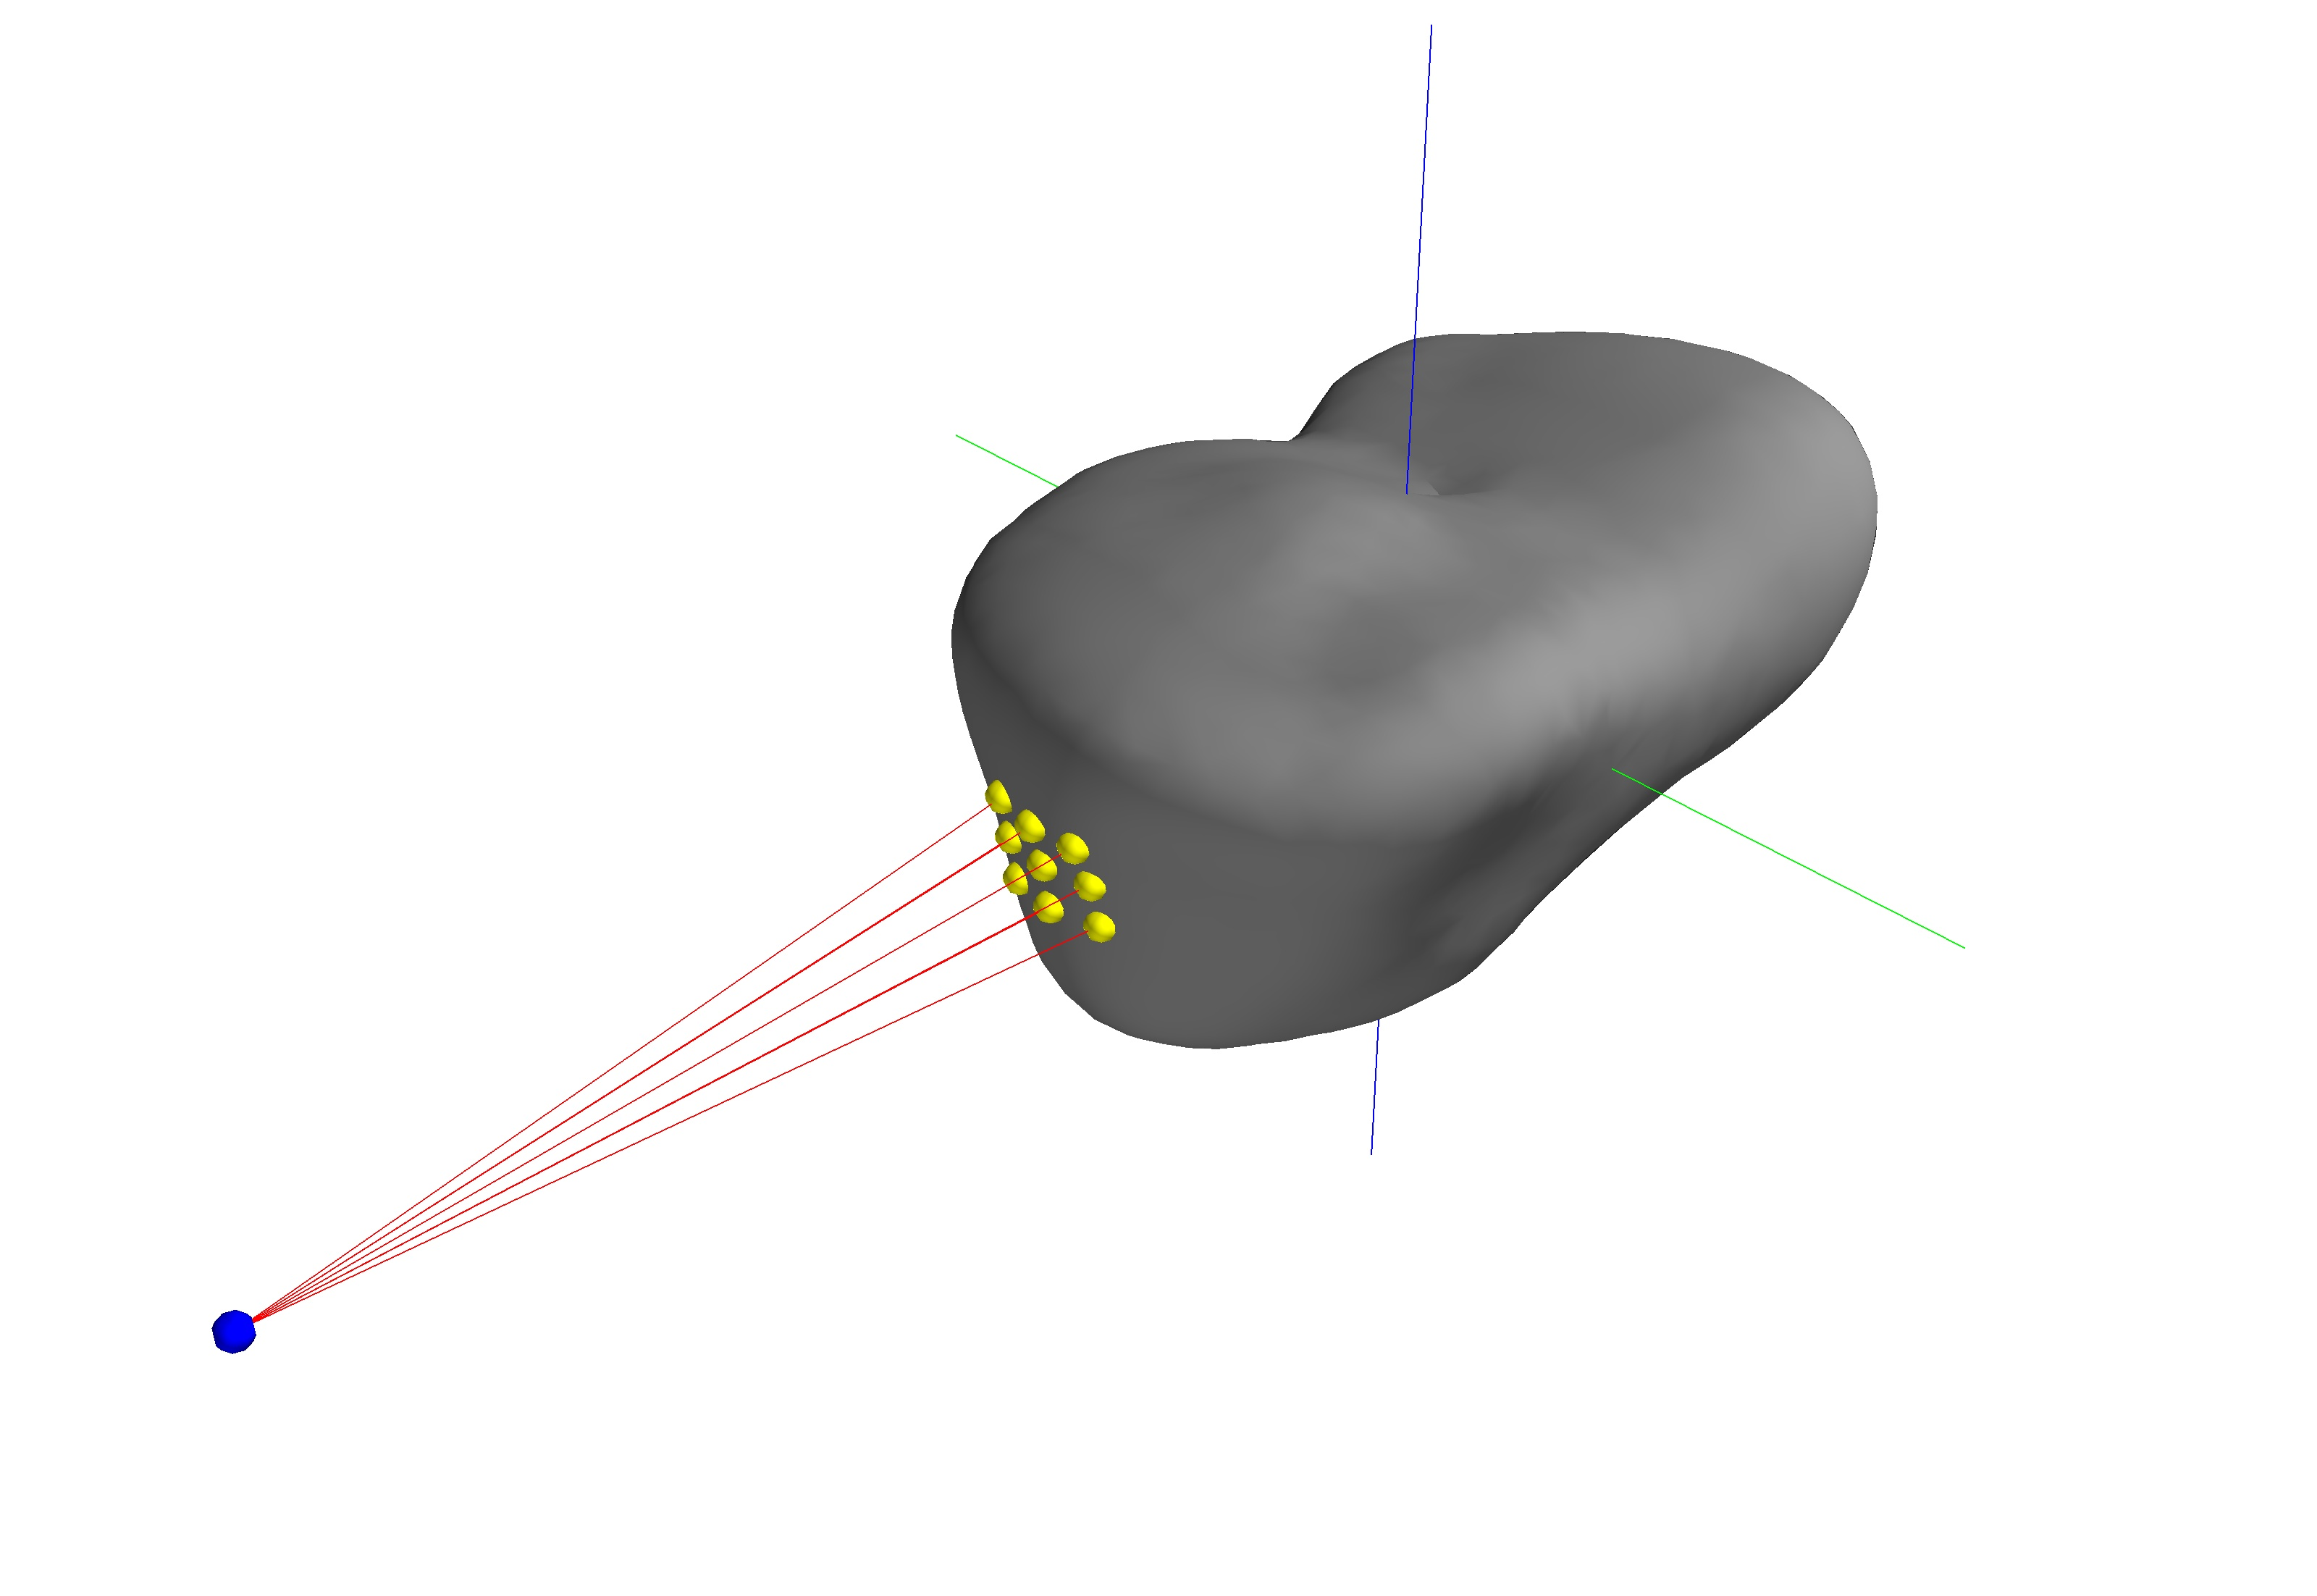
\includegraphics[width=0.75\textwidth]{figures/castalia_raycasting_plot.jpg}
    \caption{Simulated LIDAR measurements of asteroid Castalia~\label{fig:lidar_example}}
\end{figure}

\paragraph{Bayesian Shape Update}

Our algorithm applies a Bayesian framework to radially modify each vertex \( \vc{v}_i \in \R^3\) of the shape estimate based on measurement \( \vc{p}_i \in \R^3 \). 
This approach alleviates much of complexity of incorporating new vertices or surface triangulation common in surface reconstruction methods~\cite{berg2008}.
This assumption means that the total number of vertices of the shape model is fixed.
However, additional detail, in the form of additional vertices, is possible by using standard mesh subdivision algorithms~\cite{orourke1998}.

The radial distance of each vertex, \( v_i = \norm{\vc{v}_i}\), is assumed to be distributed according to the Gaussian distribution
\begin{align*}
    v_i \sim \mathcal{N}(r_i, w_i^2)
\end{align*}
where \( r_i \) is the initial estimate of the radial distance of vertex \( \vc{v}_i\) and \( w_i \) is the initial variance, or confidence, in the radial distance.
The radial distance of each measurement, \( p_{j,i} = \norm{\vc{p}_j}\), is also assumed to be distributed according to the Gaussian distribution
\begin{align*}
    p_{j,i} \sim \mathcal{N}(r_{j,i}, w_{j,i}^2)
\end{align*}
where \( r_{j,i} = \norm{\vc{p}_{j,i}} \) defines the radial distance of the surface vector measurement and \( w_{j, i}\) defines the variance of the measurement with respect to vertex \( \vc{v}_i\).
Each measurement is defined by the index \( j \) while the associated vertex is defined by \( i \). 
As a result, the measurement \( p_{j, i} \) defines the distribution of measurement \( j \) with respect to vertex \( i \). 
Any given measurement may be used to update one or several vertices.

The variance for each measurement vector is assumed to be related to the ``distance'' from the measurement to vertex \( \vc{v}_i \).
Here, we use the geodesic distance to parameterize the difference, and hence  uncertainty, of associating the measurement with a given vertex.
From spherical trigonometry~\cite{gade2010}, the central angle between measurement \( \vc{p}_i \) and vertex \( \vc{v}_i \) of the shape estimate is
\begin{align}\label{eq:geodesic_distance}
    \Delta \sigma_{j,i} = \arctan \parenth{\frac{\norm{\vc{p}_j \times \vc{v}_i}}{\vc{p}_j \cdot \vc{v}_i }}.
\end{align}
The variance of measurement \( \vc{p}_i \) with respect to vertex \( \vc{v}_i \) is then defined by the geodesic distance as
\begin{align}
    w_{j, i} = \norm{\vc{p}_j} \Delta \sigma_{j,i} .
\end{align}
This approach relates the uncertainty of the measurement \( \vc{p}_j \) with the geodesic distance to a given vertex, \( \vc{v}_i \).
As a result, measurements which are far from a vertex, i.e.\ \( \Delta \sigma \) is large, will tend to have a larger variance and hence uncertainty. 
This approach can be considered as a form of a correlation based sensor model~\cite{thrun2005}.
The main benefit of a correlation based approach, in contrast to feature extraction is the relative simplicity of implementation.
However, the resulting correlation values do not posses any physical significance and do not represent the noise or uncertainty characteristics of the sensor.

From Bayes' theorem, the posterior probability is defined as
\begin{align}
    p(v_i | p_{j, i}) = \frac{p(p_{j, i} | v_i) p(v_i)}{p( p_{j, i})} \propto p(p_{j,i} | v_i) p(v_i).
\end{align}
From the properties of a Gaussian, the posterior probability given a measurement is also distributed according to a Gaussian distribution~\cite{bishop2006} and given by
\begin{align}\label{eq:posterior_probability}
    \mathcal{N} \parenth{\frac{w_{j, i}^2 r_i + w_i^2 r_{j, i}}{w_i^2 + w_{j, i}^2} , \frac{w_i^2  w_{j, i}^2}{w_i^2 +  w_{j, i}^2}} .
\end{align}
From~\cref{eq:posterior_probability}, the posterior probability conditioned on the measurement is the weighted average of the prior knowledge and the measurement. 
Measurements that are far from the vertex will have a high uncertainty or variance and will have a reduced impact on the radial position of the vertex.
Additional measurements are incorporated using a weighted average of prior belief and the measurement uncertainty.

In order to improve the computational efficiency measurement updates are assumed to be local in nature.
Instead of applying a measurement to all vertices of the mesh, the measurement is only applied to the vertices which are within a specified region of the measurement. 
We define a region of interest, \( \Delta S \), about each measurement which defines the surface area over which the measurement will affect the mesh estimate.
We relate \( \Delta S \) to an equivalent angular constraint using
\begin{align}\label{eq:region_of_interest}
    \Delta \sigma_{max} = \sqrt \frac{\Delta S}{r_b^2}
\end{align}
% shankar: brillouin is correct. https://arc.aiaa.org/doi/10.2514/6.2014-4302
where \( r_b \) defines the Brillouin  sphere radius, or the radius of the circumscribing sphere of the asteroid.
Only vertices which satisfy \( \Delta \sigma_i \leq \Delta \sigma_{max} \) are considered in the Bayesian update shown in~\cref{eq:posterior_probability}.

The approach presented in this section allows one to update the shape of small body given a single range measurement of the surface.
A sequential process can be used to iteratively update the shape estimate given many measurements of the surface. 

\section{Optimal Guidance for Shape Reconstruction}\label{sec:explore_asteroid}

The mesh update algorithm presented does not offer a method to determine which portion of the surface needs to be updated. 
In this section, we present an optimal approach for the guidance of the vehicle in order to update the shape estimate.
A nonlinear geometric controller is utilized which allows the spacecraft to maneuver to the best location that will update the shape estimate~\cite{kulumani2017b}.
This guidance schemes enables autonomous operations around a small body.

We define a cost associated with each vertex \( \vc{v}_i \) of the shape estimate
\begin{align}\label{eq:explore_cost}
    J_i (x, R, R_A) = \alpha_w J_{w_i} + \alpha_d J_{d_i}(x_r) + \alpha_c J_{c_i}(x_r)
\end{align}
where the weighting factors \( \alpha_w, \alpha_d, \alpha_c \in \R^1 \) are chosen such that \( \alpha_w + \alpha_d + \alpha_c = 1 \).
The cost function is defined as a function of the current inertial position, \( x \in \R^3 \), and the attitude, \( R \in \R^{3\times3}\) of the spacecraft.
Furthermore, knowledge of the small body rotation is required in order to determine the position of the spacecraft in the small body fixed frame, \( x_r = R_A^T x\).

The term \( J_{w_i} \in \R^1 \) represents the cost associated with the uncertainty of vertex \( i \) as
\begin{align}\label{eq:weight_cost}
    J_{w_i} &= - \frac{w_i}{w_m}
\end{align}
where \( w_i \) is the uncertainty of vertex \( i \) and \( w_m \) is a maximum uncertainty used to scale the values.
The term \( J_{d_i} \) represents the scaled geodesic distance between the current state of the spacecraft and vertex \( i \),
\begin{align}\label{eq:distance_cost}
    J_{d_i}(\rpos) &= \frac{1}{\pi} \arctan \parenth{ \frac{\norm{\rpos \times \vc{v}_i}}{\rpos \cdot \vc{v}_i}}.
\end{align}

Finally, a control component is included in the cost function which penalizes vertices that are difficult to reach.
Consider, the current position of the spacecraft in the small body fixed frame as \( \rpos\) and a desired vertex \( \vc{v}_i \) of the shape estimate.
We can define a normal vector to the plane spanned by \( \rpos, \vc{v}_i \) as
\begin{align}\label{eq:normal_to_plane}
    \vc{n}_i = \frac{\rpos \times \vc{v}_i}{\norm{\rpos} \norm{\vc{v}_i}}.
\end{align}
Then a trajectory \( x_d(\theta) \) as
\begin{align}\label{eq:spherical_waypoint}
    x_d(\theta) = r_d \exp{\parenth{\theta \hat{\vc{n}_i}} } \frac{\rpos}{\norm{\rpos}},
\end{align}
where \( \theta : \bracket{0, \frac{\rpos \cdot \vc{v}_i}{\norm{\rpos}\norm{\vc{v}_i}}} \to \R^1\) parameterizes the desired trajectory.
\Cref{eq:spherical_waypoint} simply describes a portion of a great circle trajectory between the current state, \( \rpos \), and the desired vertex \( \vc{v}_i \)~\cite{chen2016}.
The altitude of the spacecraft, \( r_d \in \R \), can be chosen based on sensor characteristics of safety concerns.
For example, \( r_d \) can be chosen as the distance of the Biroullin sphere with an additional safety margin to mitigate any surface collision~\cite{scheeres2012a}.
We assume that the tracking errors are small, such that \( e_x, e_v \) are negligible, therefore the control becomes
\begin{align}\label{eq:tracking_control_cost}
    u_f(\theta) = -F_{ext}(x_d(\theta)), 
\end{align}
where the external force is defined by the polyhedron potential model given in~\cref{eq:attraction}.
The control cost is then defined as the integral over the desired trajectory~\cref{eq:spherical_waypoint} between the current state and the desired vertex as
\begin{align}\label{eq:control_cost}
    J_{c_i}(\rpos) = \frac{1}{u_m} \int_{\theta_0}^{\theta_f} u_f(\theta)^T R u_f(\theta) d\theta,
\end{align}
where \( u_m \) is used to normalize and scale \( J_{c_i} \).
\Cref{eq:control_cost} is numerically integrated over the trajectory \( x_d(t) \) and used to penalize vertices which have a larger cost.

The vertex which minimizes~\cref{eq:explore_cost} 
\begin{align*}
    \vc{v}_{min} = \min_{i} J_i(x, R, R_A),
\end{align*}
is determined and used to determine the optimum vertex of the shape model to measure.
This vertex is then used to determine the required state of the spacecraft in order to collect a measurement.
We assume that the spacecraft will maneuver to a location directly above the selected vertex, \( \vc{v}_{min} \), and point in the nadir direction to collect a measurement.
The desired state is transformed into the inertial frame and chosen as a location above \( \vc{v}_{min} \) as
\begin{align}
    x_d = r_d R_A \vc{v}_{min}, 
\end{align}
where \( r_d \) is again chosen to ensure a safety margin above the surface.
The desired attitude command, \( R_d\), is chosen such that the spacecraft camera axis, \( \vc{b}_1 \), is directed along the nadir towards the small body.
It is sufficient to define two orthogonal vectors to uniquely determine the attitude of the spacecraft.
The \( \vc{b}_{3d} \) vector is chosen to lie in the plane spanned by \(\vc{b}_{1d} \) and \( \vc{e}_3 = \vc{f}_3 \).
The desired attitude command is defined as
\begin{align}
    \vc{b}_{1d} &= - \frac{\vc{x}}{\norm{\vc{x}}} , \\
    \vc{b}_{3d} &= \frac{\vc{f}_3 - \parenth{\vc{f}_3 \cdot \vc{b}_{1d}} \vc{b}_{1d}}{\norm{\vc{f}_3 - \parenth{\vc{f}_3 \cdot \vc{b}_{1d}} \vc{b}_{1d}}}, \\
    \vc{b}_{2d} &= \vc{b}_{3d} \times \vc{b}_{1d} , \\
    R_d &= \begin{bmatrix} \vc{b}_{1d} & \vc{b}_{2d} & \vc{b}_{3d} \end{bmatrix} .
\end{align}
This form of \( R_d \) will direct the \( b_1 \) axis towards the small body, and can be modified for a different camera orientation.


\section{Multi-resolution Landing Area Refinement}\label{sec:landing_refinement}

The shape update approach presented is designed with autonomous operations in mind. 
It is based on an initial coarse shape estimate that is iteratively updated with range measurements of the surface.
Furthermore, the original mesh is uniformly distributed and as a result many small topological features such as rocks or small craters are not be captured by the shape model. 
However, these small features are critical for surface operations and safe landings.
In addition, it would be computationally prohibitive to have a uniformly high resolution mesh.
In this section, we extend the previous shape update approach to enable a much higher fidelity in a specific location.

Mixed resolution surface meshes are routinely used in finite element and geometric modeling applications~\cite{botsch2010}.
As shown in Reference~\citenum{mcmahon2017}, utilizing mixed resolution shape models for asteroid missions offers the potential of reduced computational demands.
The computational cost of the polyhedron potential model, given by~\cref{eq:potential}, is roughly proportional to the number of faces in the shape model.
As a result, a uniformly high resolution shape would quickly become intractable for real time operations.
However, utilizing a mixed resolution approach allows for a high fidelity in a smaller mission critical area, such as a landing site, with a limited impact on the computational cost.

The selection of a landing site will typically require a vast quantity of data and weigh a multitude of possible metrics, such as scientific value, hardware constraints, timing and communication limits, or safety considerations. 
In our analysis we consider the surface slope, the distance to the surface, and a fictitious science metric in order to determine the best landing site based on the complete shape estimate.
This approach allows for a spacecraft to autonomously select and land on small body.

The surface slope is computed according to the method developed in Reference~\cite{scheeres1996}.
Due to the small size, and therefore low gravitational attraction, the force at each point on the surface is a combination of the gravitational attraction and the centripetal acceleration.
At the center of each face, \( f_i = \begin{bmatrix} f_x & f_y & f_z \end{bmatrix} \), we compute a modified surface acceleration as
\begin{align}\label{eq:surface_force}
    U_m = \omega^2 \begin{bmatrix} f_x \\ f_y \\ 0 \end{bmatrix} + \begin{bmatrix} U_x \\ U_y \\ U_z \end{bmatrix},
\end{align}
where \( \omega \in \R^1 \) is the angular velocity of the asteroid and \( U_i \) is computed from~\cref{eq:attraction}.
Then the surface slope can be computed from
\begin{align}\label{eq:surface_slope}
    \cos \parenth{ \pi - \phi } = \frac{\vc{n}_f \cdot U_m}{\norm{U_m}},
\end{align}
where \( \phi \in \R^1 \) is the surface slope defines the angle between the surface normal \( \vc{n}_f \in \R^3 \) and the force vector at the surface.
If \( \phi = \SI{0}{\degree} \) then the force vector and the surface normal are anti-parallel, while \( \phi > \SI{90}{\degree} \) means that a particle on the surface would be thrown off the body as the centripetal force is larger than the gravitational attraction.

Additionally, we compute the distance, using~\cref{eq:geodesic_distance}, between the spacecraft state and each face of the asteroid. 
Finally, we also assign a random science value to the surface in the form of a two dimensional Gaussian.
Utilizing these metric, a landing site is chosen to minimize the surface cost given as
\begin{align}\label{eq:surface_cost}
    J_l =  J_{\text{distance}} - J_{\text{science}},
\end{align}
where the surface slope is considered a hard constraint such that any candidate landing site must satisfy \( \phi \leq \phi_m \).

\paragraph{Mesh Refinement}\label{sec:refinement}

Once a suitable landing site is selected, the surrounding area is isolated and refined by adding new vertices and faces in the specified area.
The goal of refinement, or more generally remeshing, is given a mesh ( or a portion of it), compute another mesh whose elements satisfy some quality metrics while suitably approximating the original mesh.
In this work, we utilize the isotropic remeshing algorithm implemented in the Computational Geometry and Algorithms Library (CGAL).
This algorithm uses an iterative method which repeatedly splits long edges, collapses short edges, and relocates vertices until all edges are approximately the desired target edge length.
% TODO Think about adding PMP 6.12 image here

For example,~\cref{fig:cube_remesh} shows the isotropic remeshing result for the selected faces of a unit cube.
The original unit cube is composed of \num{8} vertices and \num{12} faces.
The two triangular faces of the visible side of the cube are selected for the isotropic remeshing operation as shown in~\cref{fig:cube_original_mesh}.
A target edge length of \num{0.1} is selected for these faces and used to generate~\cref{fig:cube_refine_mesh}.
The two large triangular faces are divided into a number of smaller triangular faces.
Furthermore, the additional faces are all approximately the same size and preserve the original surface of the cube.
After the isotropic remeshing operation the number of vertices has increased from \num{8} to \num{140}.
\begin{figure}[htbp]
    \centering
    \subcaptionbox{Original Cube\label{fig:cube_original_mesh}}{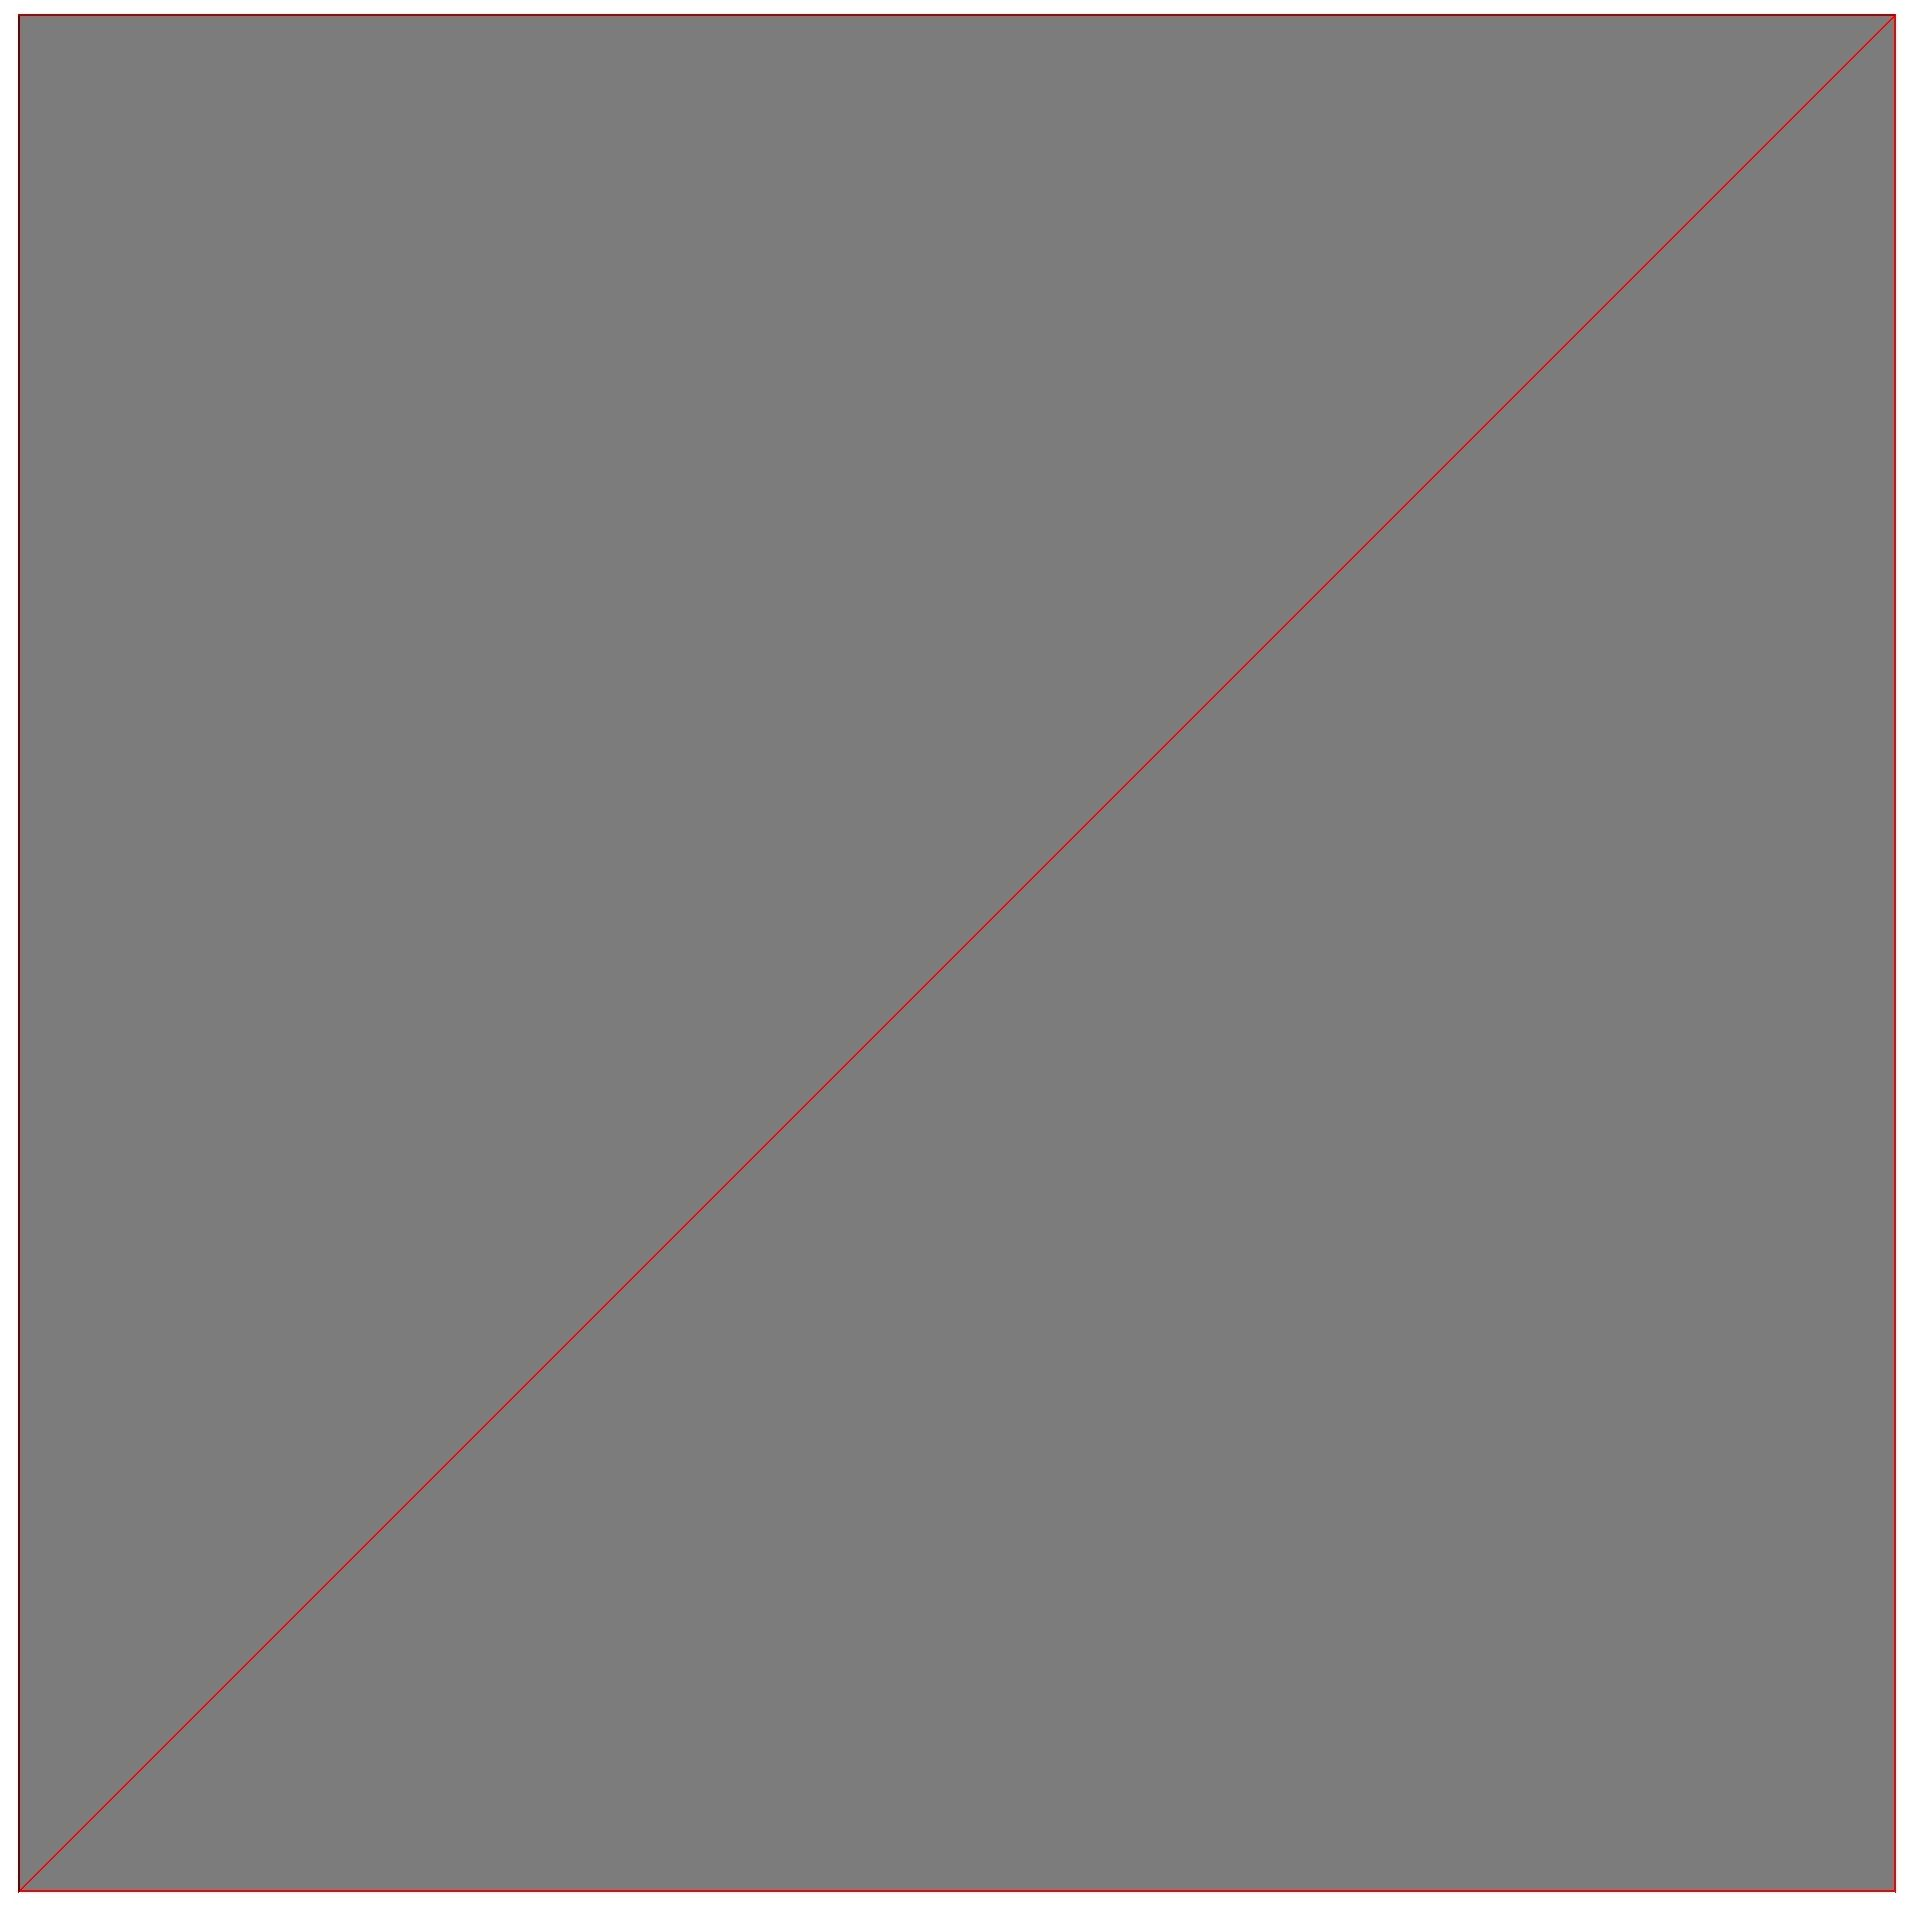
\includegraphics[width=0.25\textwidth]{figures/original_cube.jpg}}~
    \subcaptionbox{Remeshed Cube\label{fig:cube_refine_mesh}}{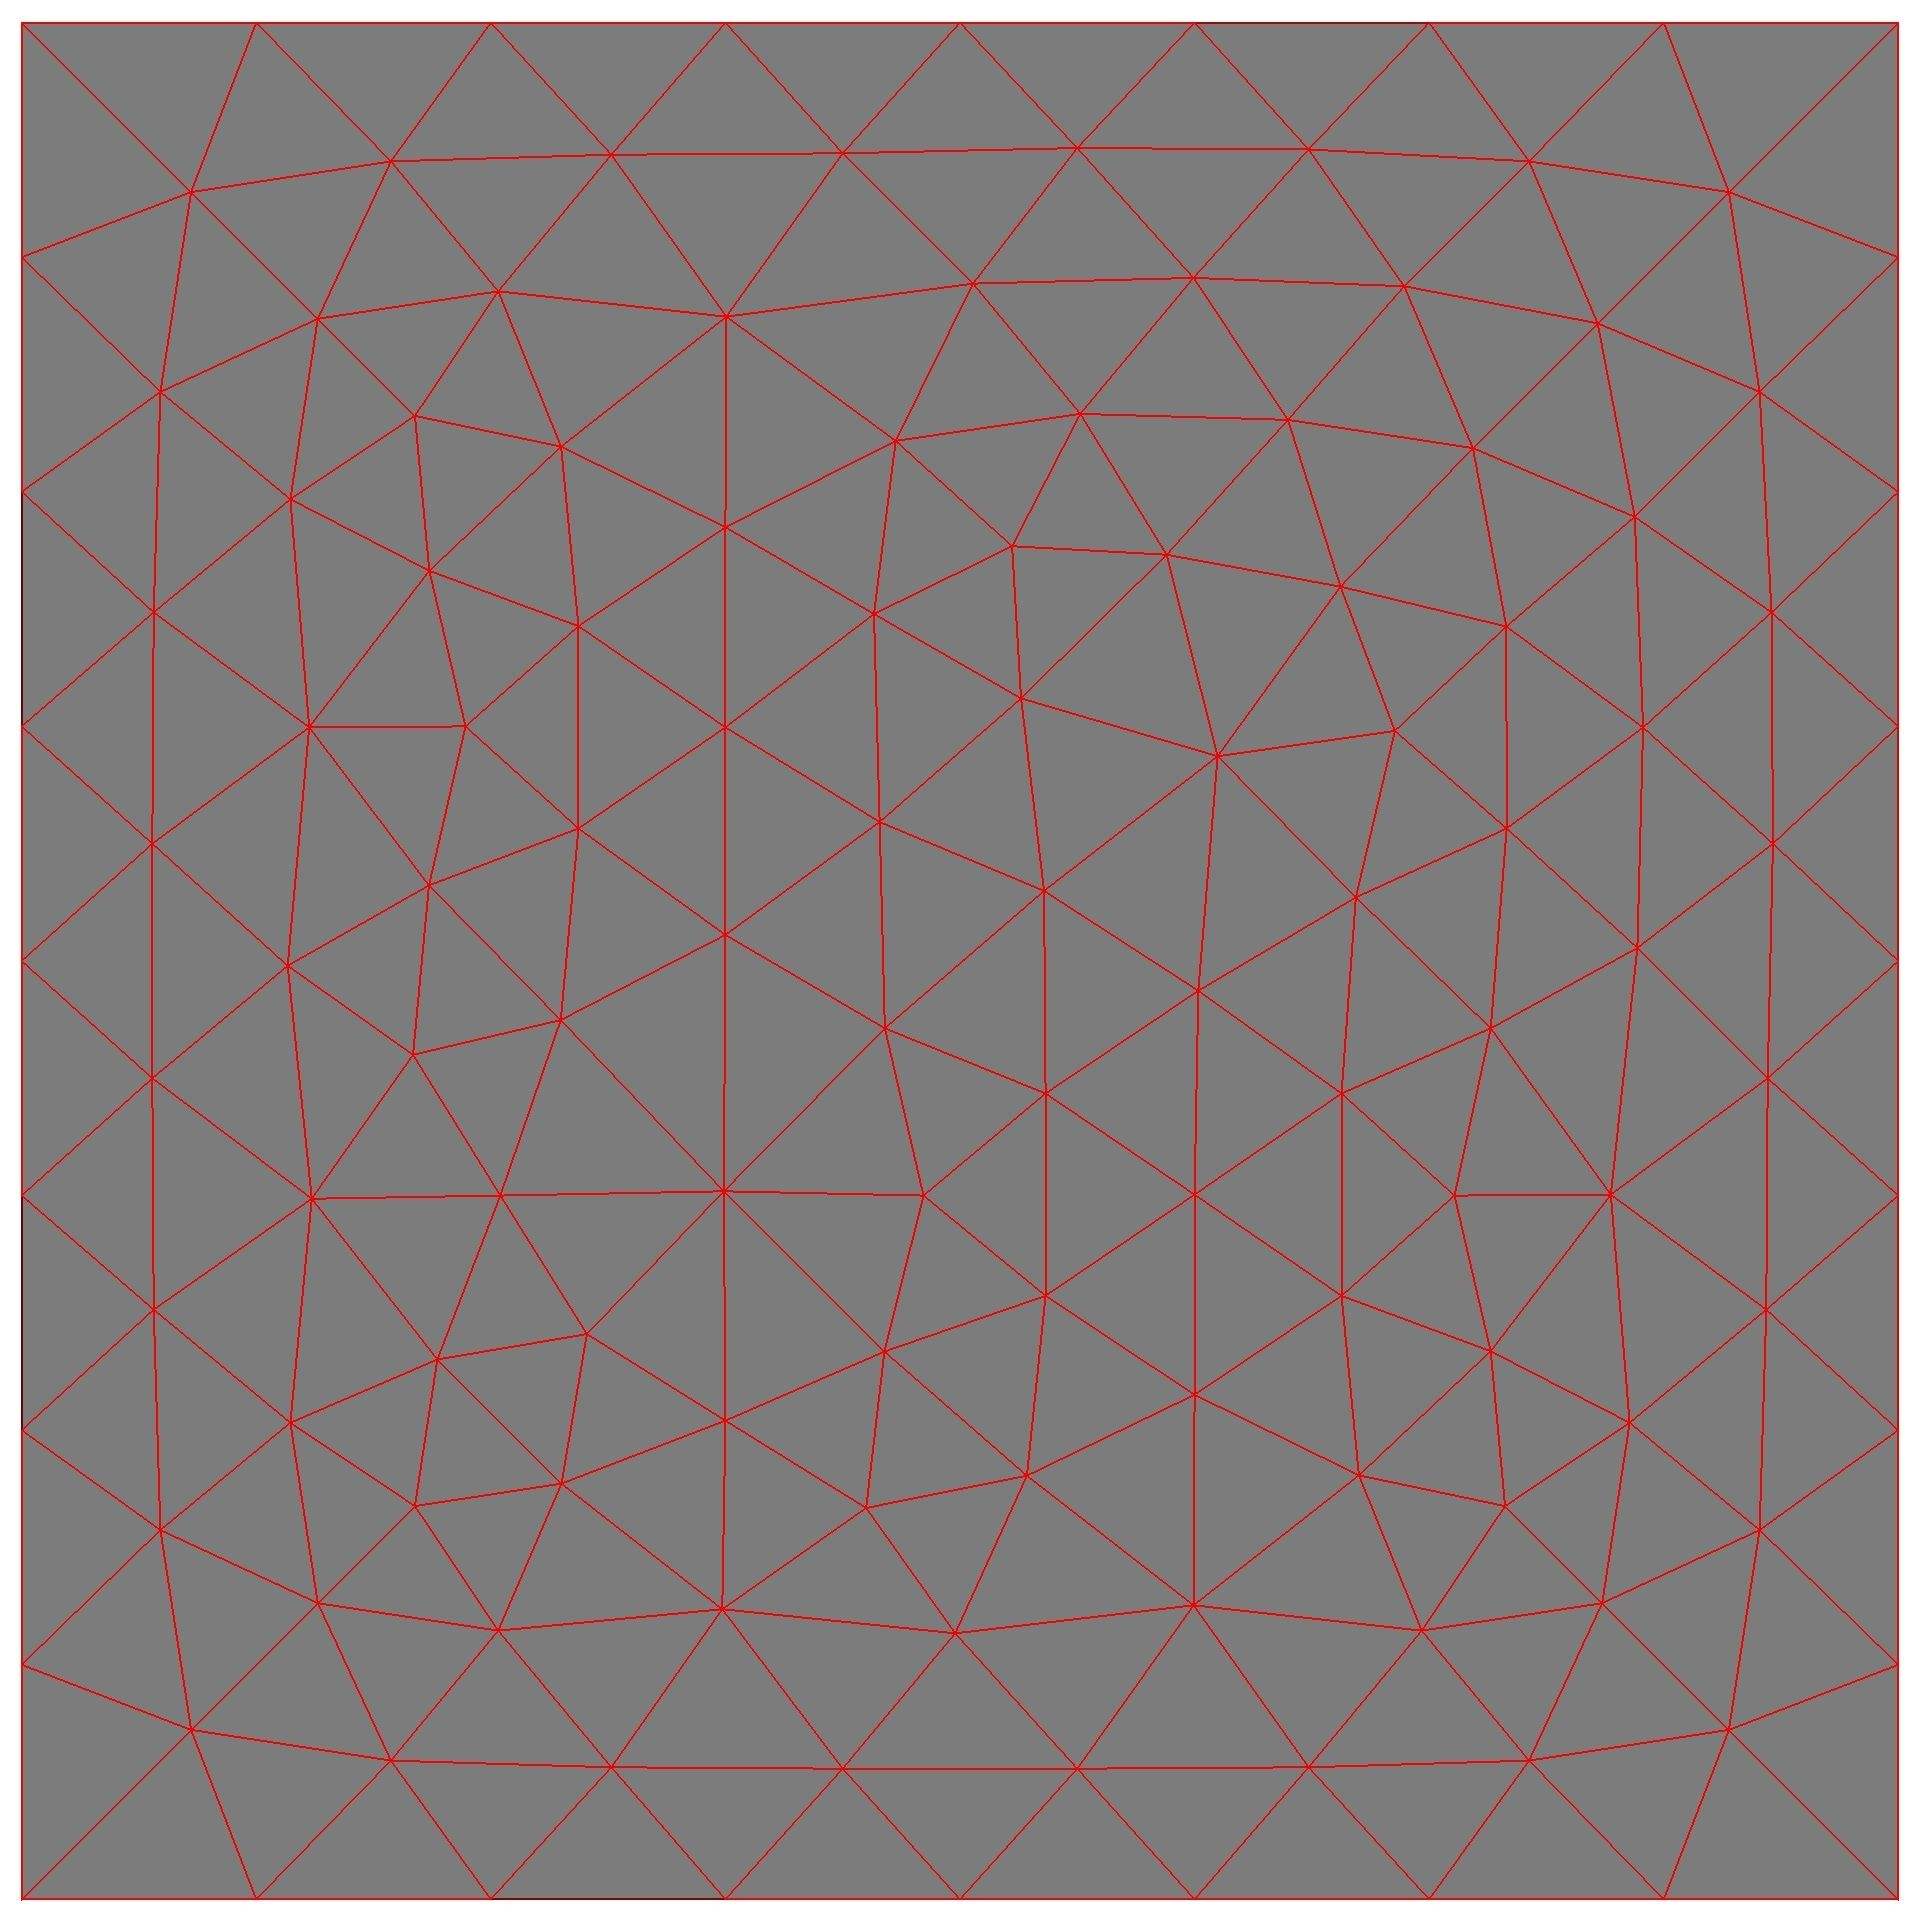
\includegraphics[width=0.25\textwidth]{figures/remesh_cube.jpg}}
    \caption{Example of isotropic remeshing of a face of a cube\label{fig:cube_remesh}}
\end{figure}

In order to demonstrate the multi resolution surface refinement we require a true shape model that contains small scale surface features.
In this dissertation, we utilize the true radar shape model of asteroid 4769 Castalia.
However, the shape model is not highly detailed as it does not contain small craters or surface features.
In order to apply the landing refinement process we augment a small portion of the mesh with some additional features and utilize the mesh update scheme shown previously to update the surface.
The augmented model of Castalia is shown in~\cref{fig:castalia_refinement}.
\Cref{fig:castalia_refinement} shows that the increased resolution is required in order to reconstruct these small surface details.


\section{Numerical Examples}\label{sec:reconstruction_examples}

% TODO Add more plots from dissertation. All the uncertainty and volume plots
% TODO Show examples with the other asteroids
% TODO Mention that the software to do this is available online?
In this section, we demonstrate the use of the incremental shape reconstruction algorithm.
The approach is used to iteratively reconstruct the shape of several asteroid given LIDAR measurements.
We utilize radar shape models of asteroids \num{4769} Castalia and (\num{52760}) \num{1998} \(\text{ML}_{14}\).
The examples demonstrate the full dynamic simulation of a rigid spacecraft with an autonomous closed loop control scheme to both reconstruct the asteroid shape.

The nonlinear controllers described previously are used to control both the translational and rotational states of the vehicle.
Throughout the simulation the control inputs are computed using the current shape estimate of the asteroid. 
As measurements are collected, the spacecraft autonomously updates its shape estimate and uses this estimate to compute the control inputs and desired future states.
These simulations demonstrate the ability of a spacecraft to autonomously explore and maneuver around an unknown small body.

We consider two simulations about asteroids \num{52760} and Castalia.
The asteroids are assumed to constantly rotate about the \( \vc{f}_3 = \vc{e}_3\) axis according to the parameters given in~\cref{tab:dynamic_asteroids}.
Furthermore, the state of the asteroid, namely the rotation matrix \( R_A \), is assumed to be known based on ground measurements or previous data.
\begin{table}[htbp]
    \centering
    \begin{tabular}{lcc}
        \toprule
        Property & \num{4769} Castalia & (\num{52760}) \num{1998} \(\text{ML}_{14}\) \\
        \midrule
        Semi-major axes(\si{\kilo\meter}) & \( 0.8065 \times 0.4905 \times 0.413 \) & \( 1.1 \times 1.1 \times 1.1 \) \\
        Rotational Period (\si{\hour}) & \num{4.095} & \num{14.98} \\
        Density (\si{\gram\per\centi\meter^3}) & \num{2.1} & \num{2.1} \\
        Vertices & \num{2048}  & \num{8192} \\
        Faces & \num{4092} & \num{16320} \\
        \bottomrule
    \end{tabular}
    \caption{Asteroid properties for dynamic exploration~\label{tab:dynamic_asteroids}}
\end{table}
At the beginning of the simulation the spacecraft is assumed to lie on the inertial \( e_1 \) axis, i.e.\ \( x_0 = \begin{bmatrix} x_0 & 0 & 0 \end{bmatrix} \si{\kilo\meter} \).
In addition, at the initial state the spacecraft is orientated such that the \( b_1 \) axis is aligned with the inertial \( e_2 \) axis.
In other words the initial orientation is given by \( R_0 = \exp(\frac{\pi}{2} \hat{e}_3)\).
The shape reconstruction phase of the simulation is performed over \SI{15000}{\second}, over which time the spacecraft will take LIDAR measurements of the surface at \SI{1}{\hertz}.
Once the total uncertainty has been reduced sufficiently the spacecraft maneuvers to a ``home'' position aligned with the \( f_1 \) axis of the asteroid.

\paragraph{Asteroid 52760 Reconstruction}

Asteroid (\num{52760}) \num{1998} \(\text{ML}_{14}\) was discovered in \num{1998} and is near Earth asteroid of the Apollo group and classified as a potentially hazardous body.
The asteroid is roughly spherical with a mean radius of approximately \SI{1}{\kilo\meter}.
The initial shape estimate is assumed to be spherical with approximately the same number of vertices as the truth model.
\Cref{fig:52760_weights_reconstruction} show the shape reconstruction at several discrete points during the simulation.
Due to the roughly spherical shape of the asteroid large portions of the surface are quickly modified to match the measurements.
In addition~\cref{fig:52760_weights_reconstruction} displays the vertex uncertainty \( w_i \) as a colormap on the surface. 
Areas of high uncertainty are denoted in yellow while areas of low uncertainty are in purple/blue.

\begin{figure}[htbp]
    \centering
    \subcaptionbox{Initial Shape Estimate\label{fig:52760_partial_weights_0}}{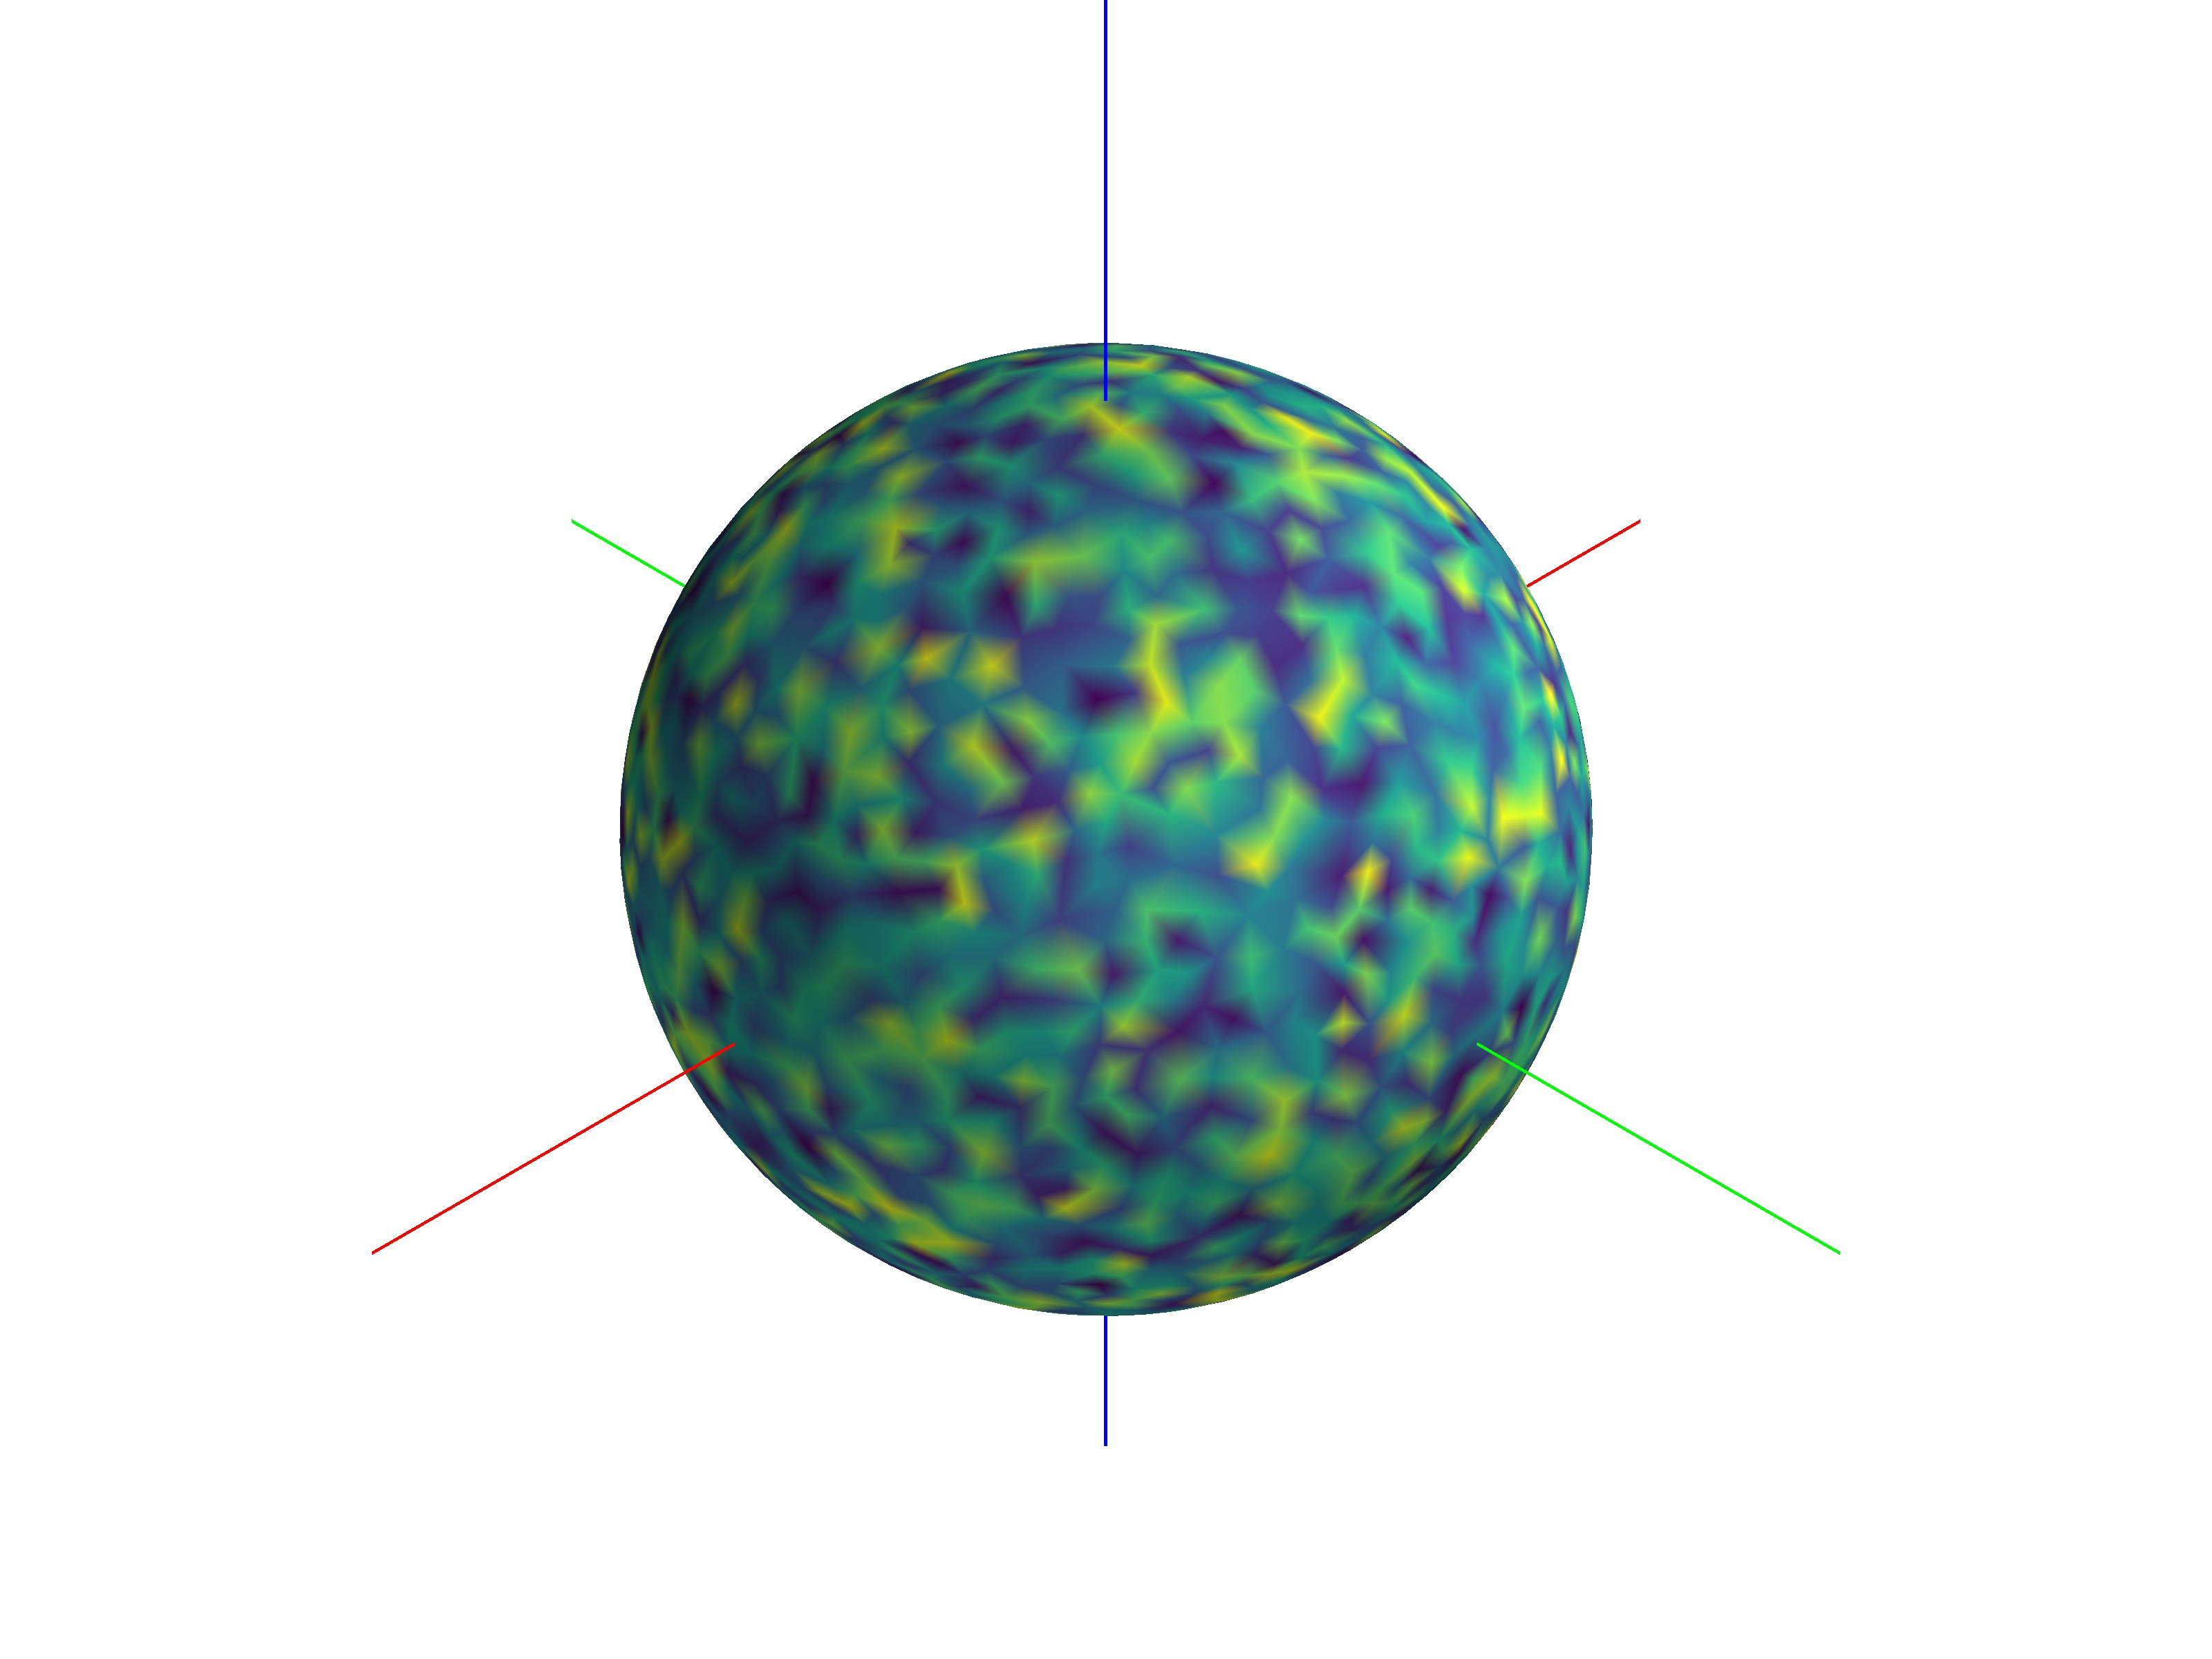
\includegraphics[trim={30cm 15cm 30cm 15cm},clip,height=0.25\textheight,width=0.3\textwidth,keepaspectratio]{figures/dynamic_exploration/52760/partial_weights_1.jpg}}%
    \subcaptionbox{\SI{25}{\percent} of measurements\label{fig:52760_partial_weights_25}}{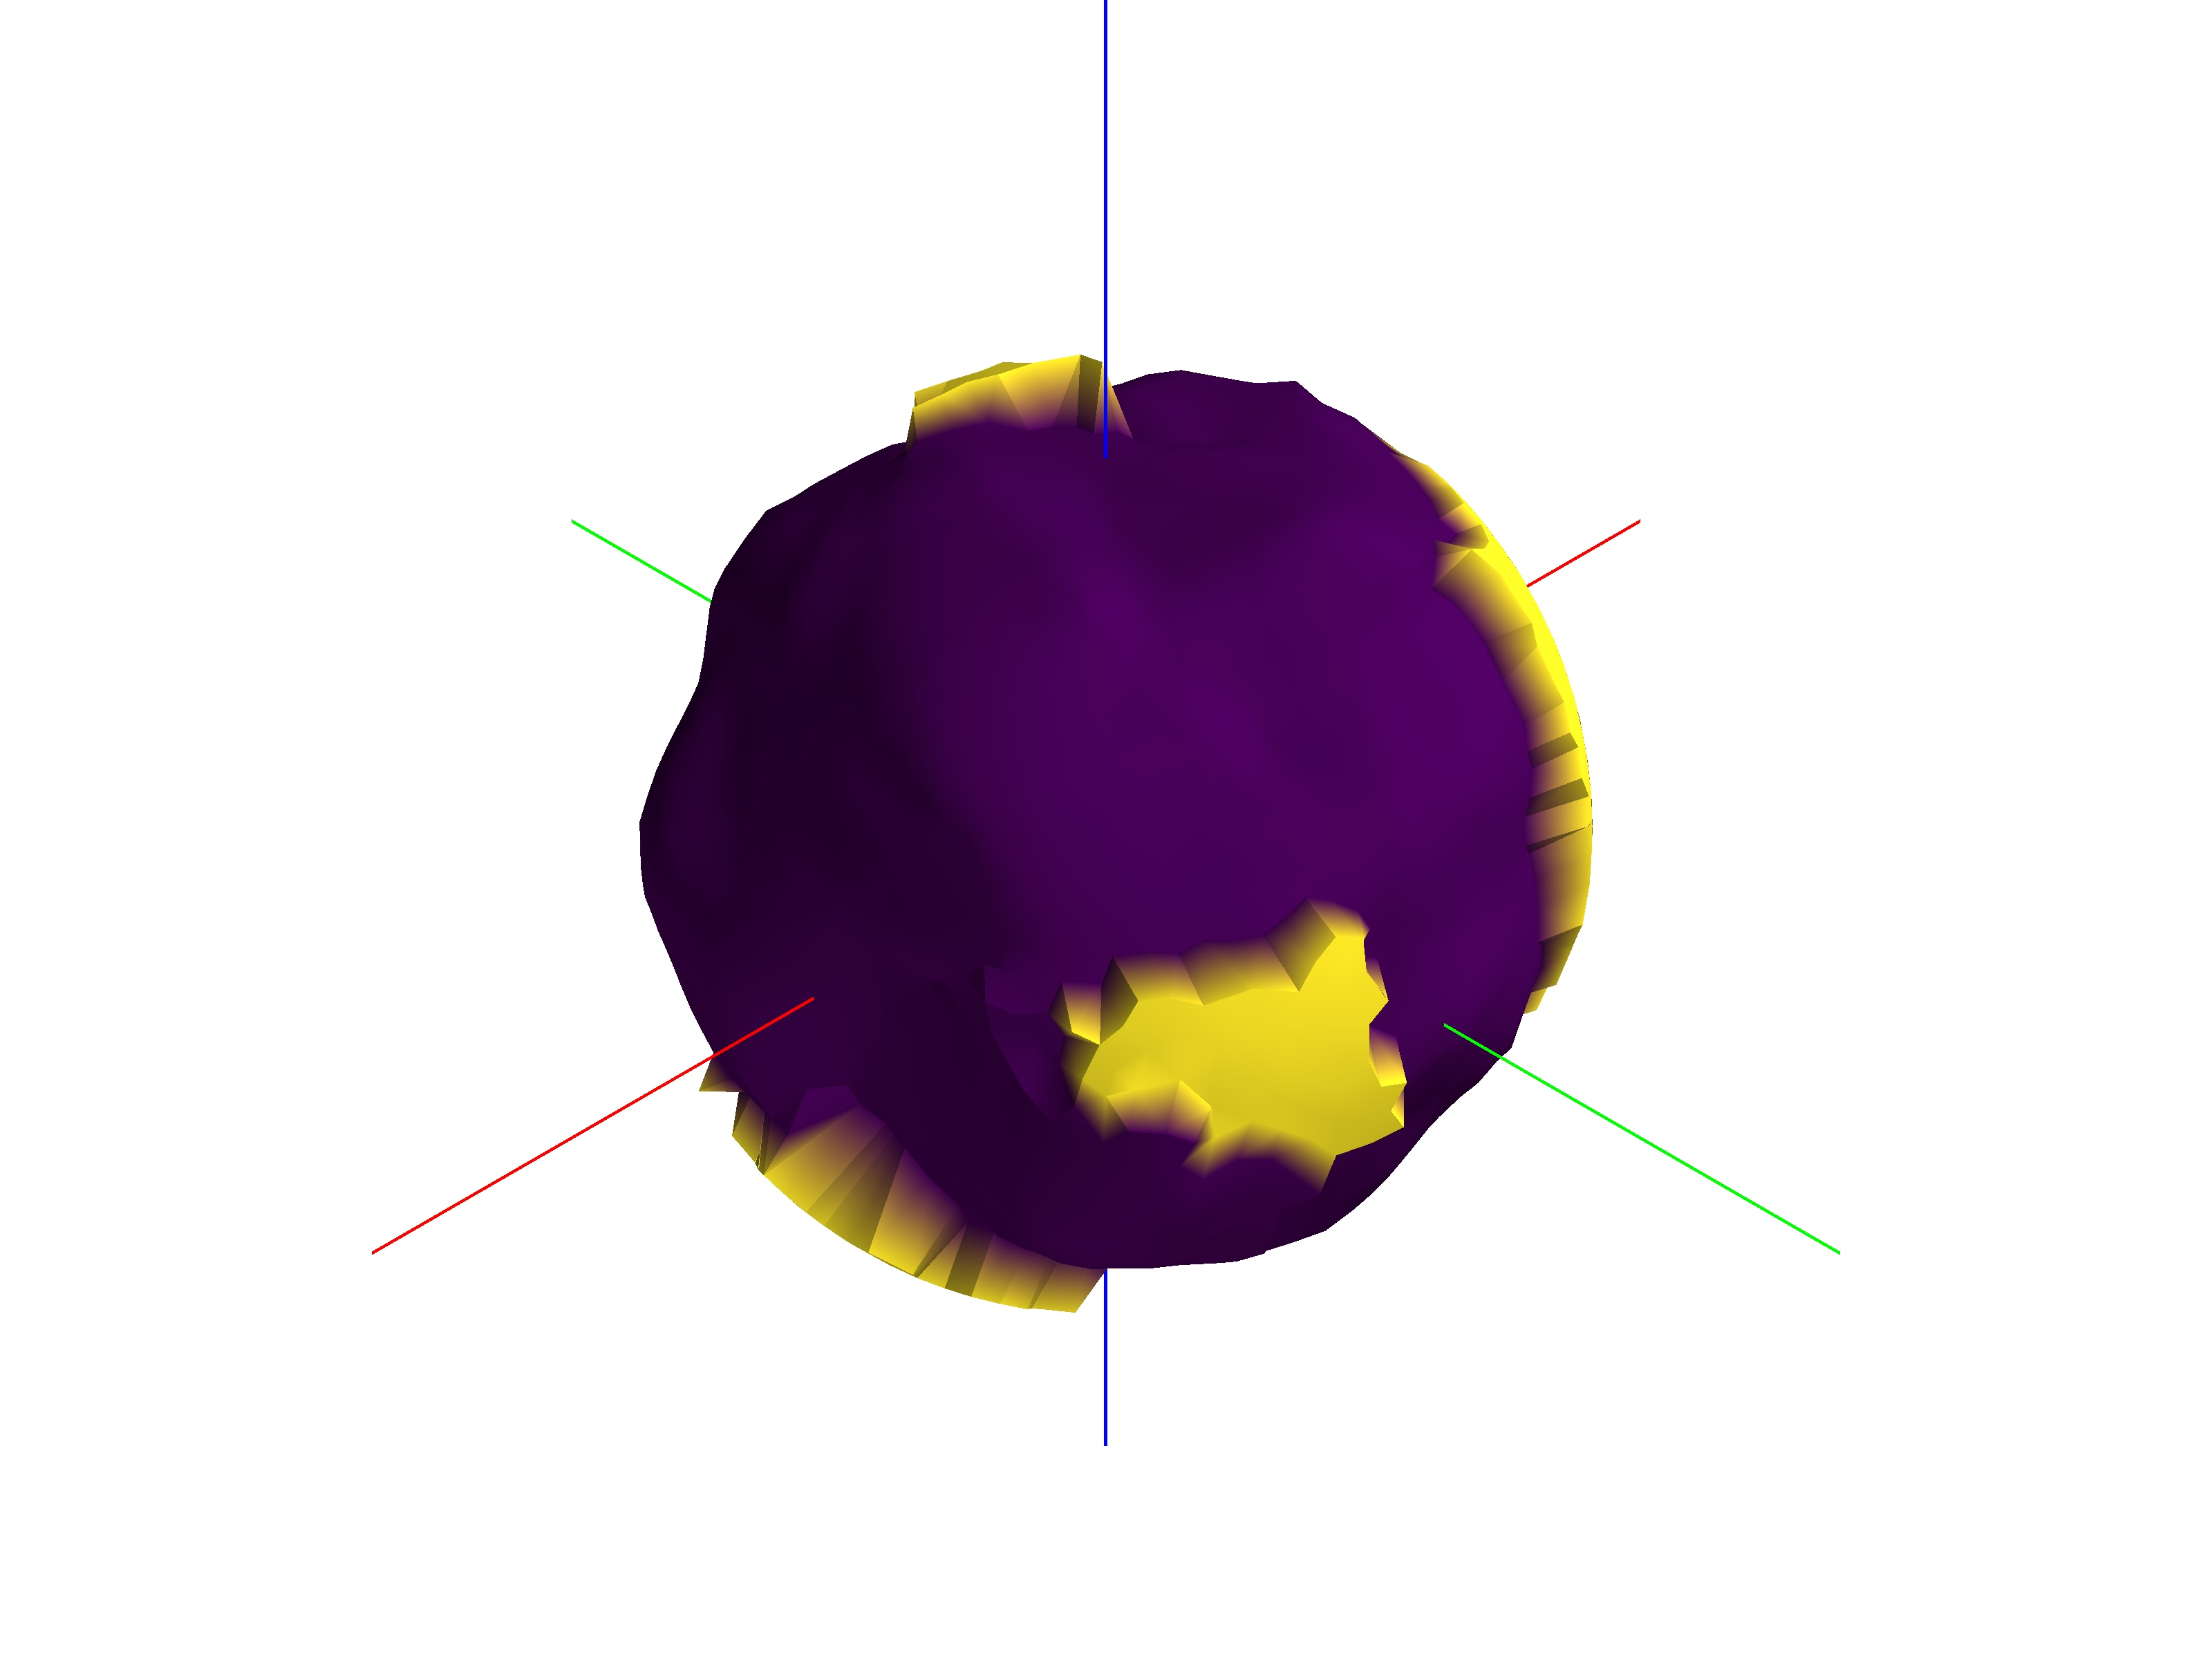
\includegraphics[trim={30cm 15cm 30cm 15cm},clip,height=0.25\textheight,width=0.3\textwidth,keepaspectratio]{figures/dynamic_exploration/52760/partial_weights_3749.jpg}}%
    \subcaptionbox{\SI{50}{\percent} of measurements\label{fig:52760_partial_weights_50}}{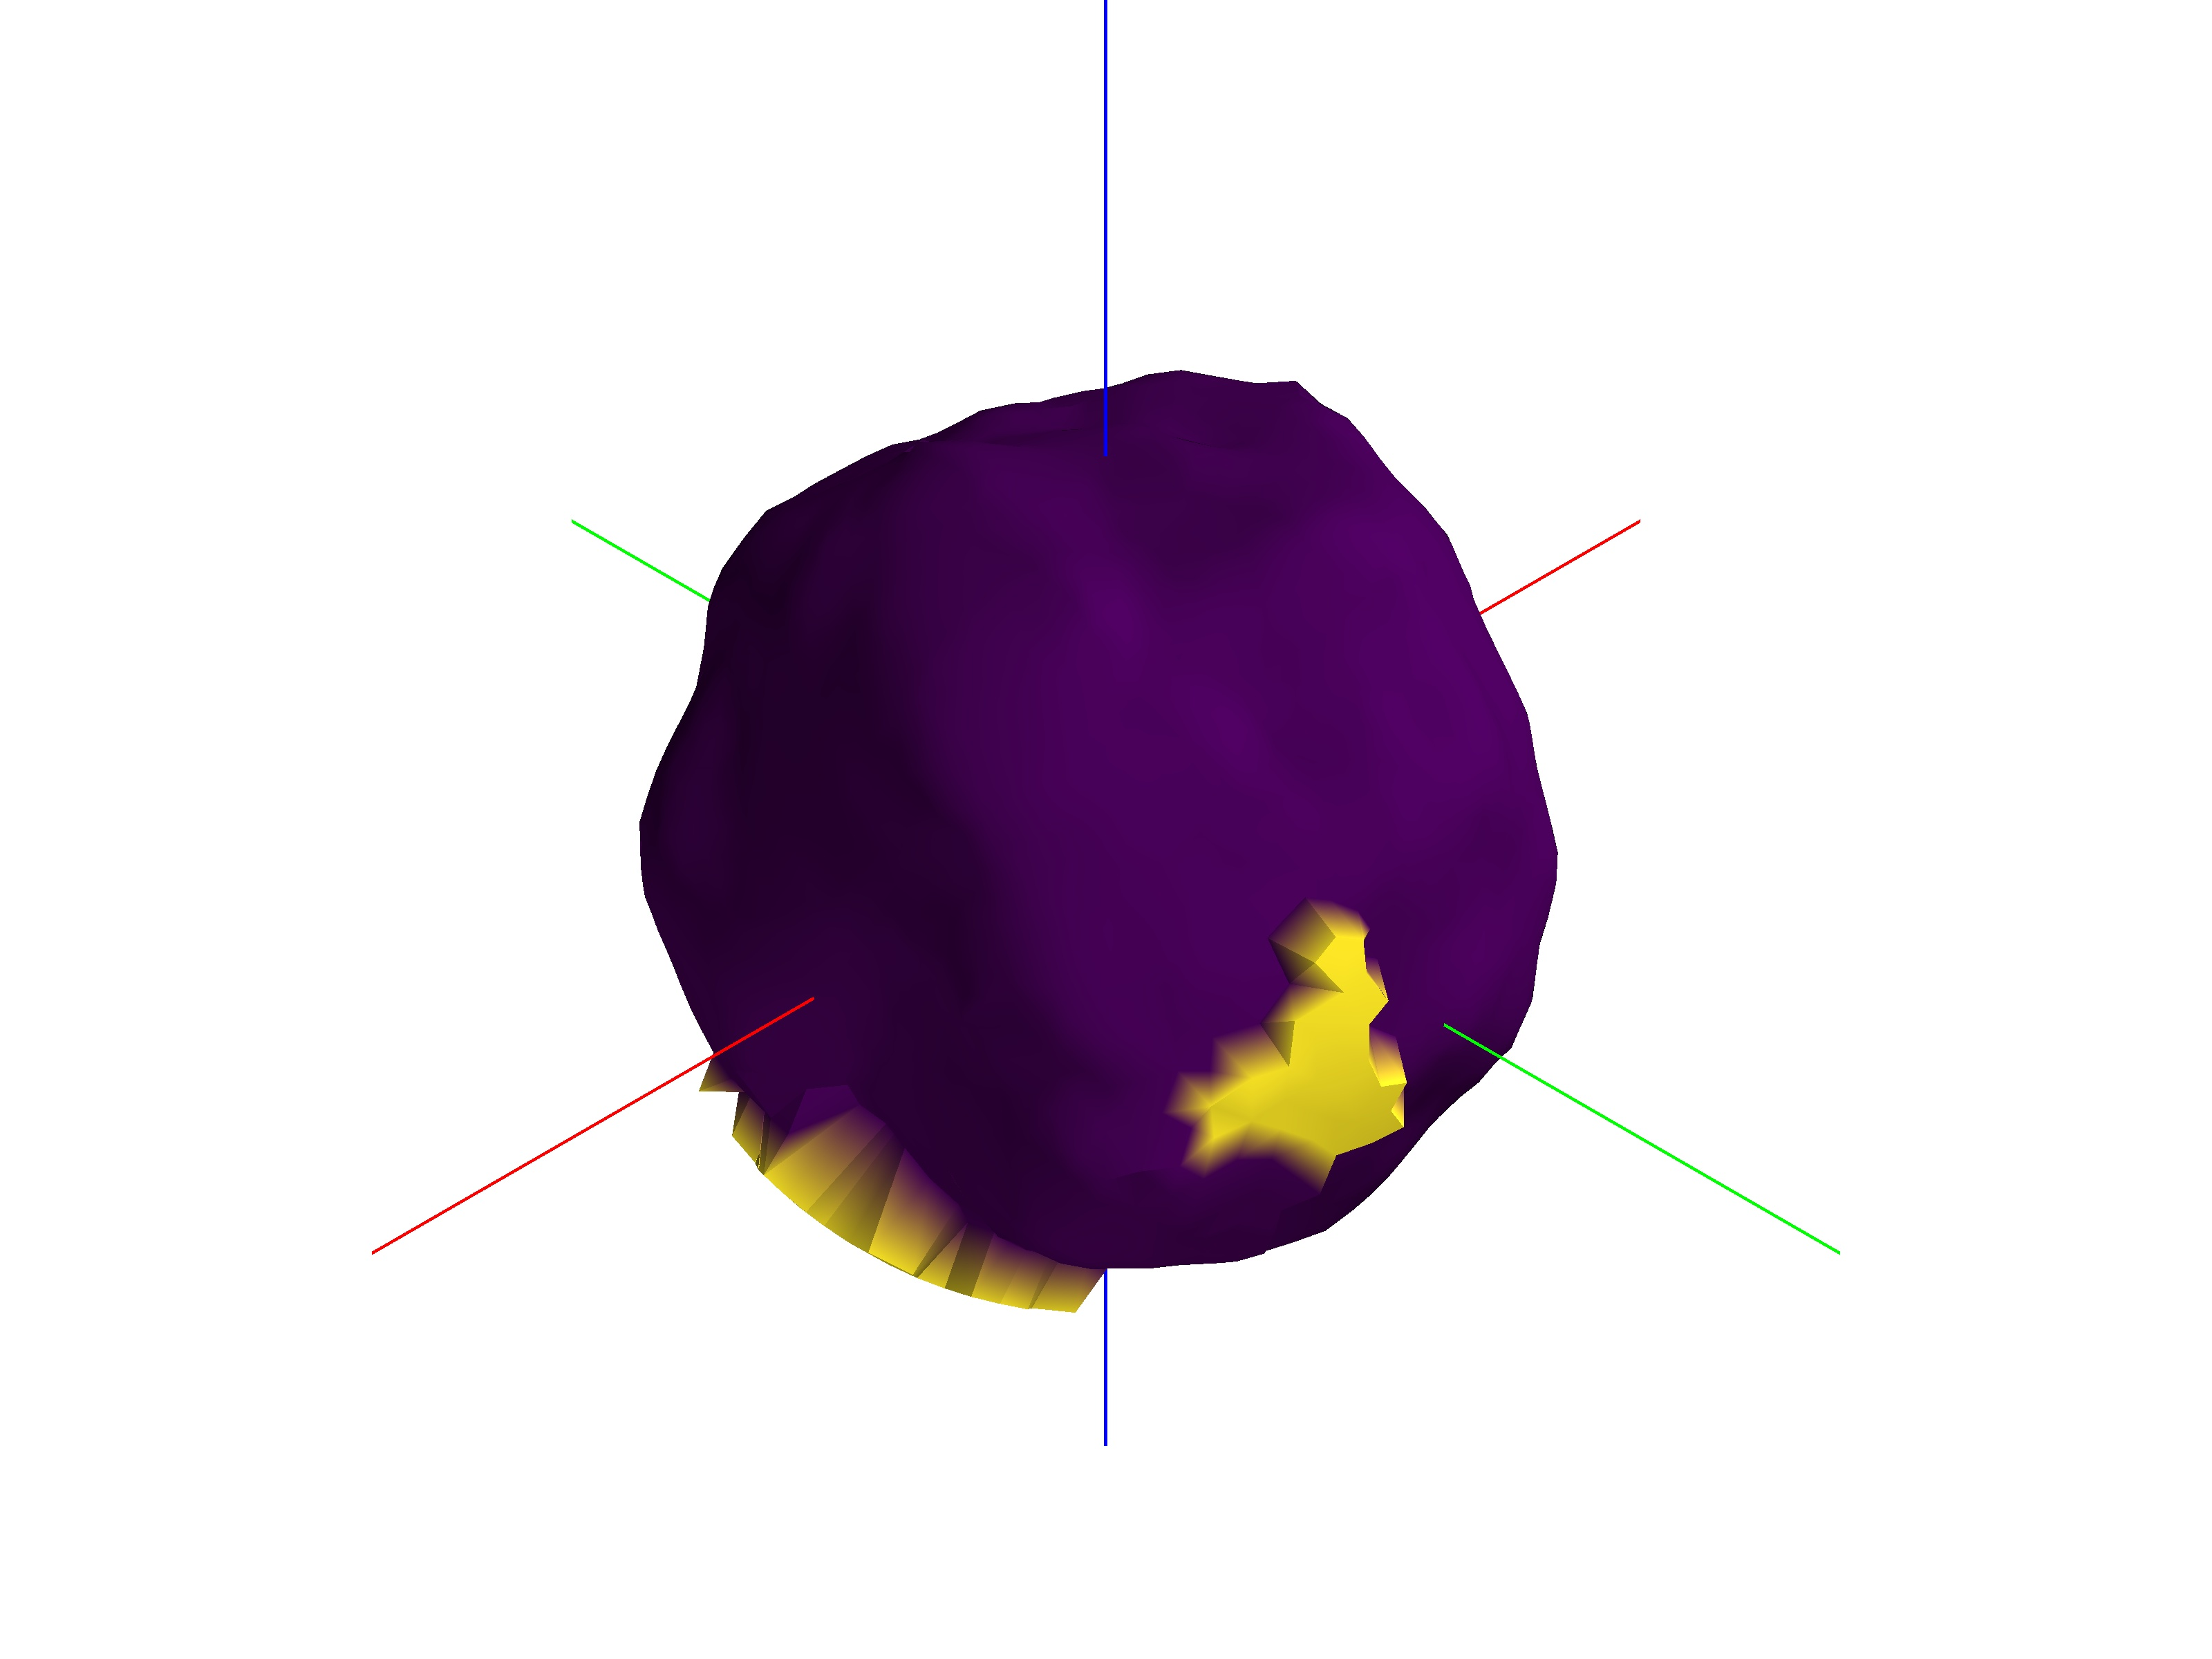
\includegraphics[trim={30cm 15cm 30cm 15cm},clip,height=0.25\textheight,width=0.3\textwidth,keepaspectratio]{figures/dynamic_exploration/52760/partial_weights_7499.jpg}}

    \subcaptionbox{\SI{75}{\percent} of measurements\label{fig:52760_partial_weights_75}}{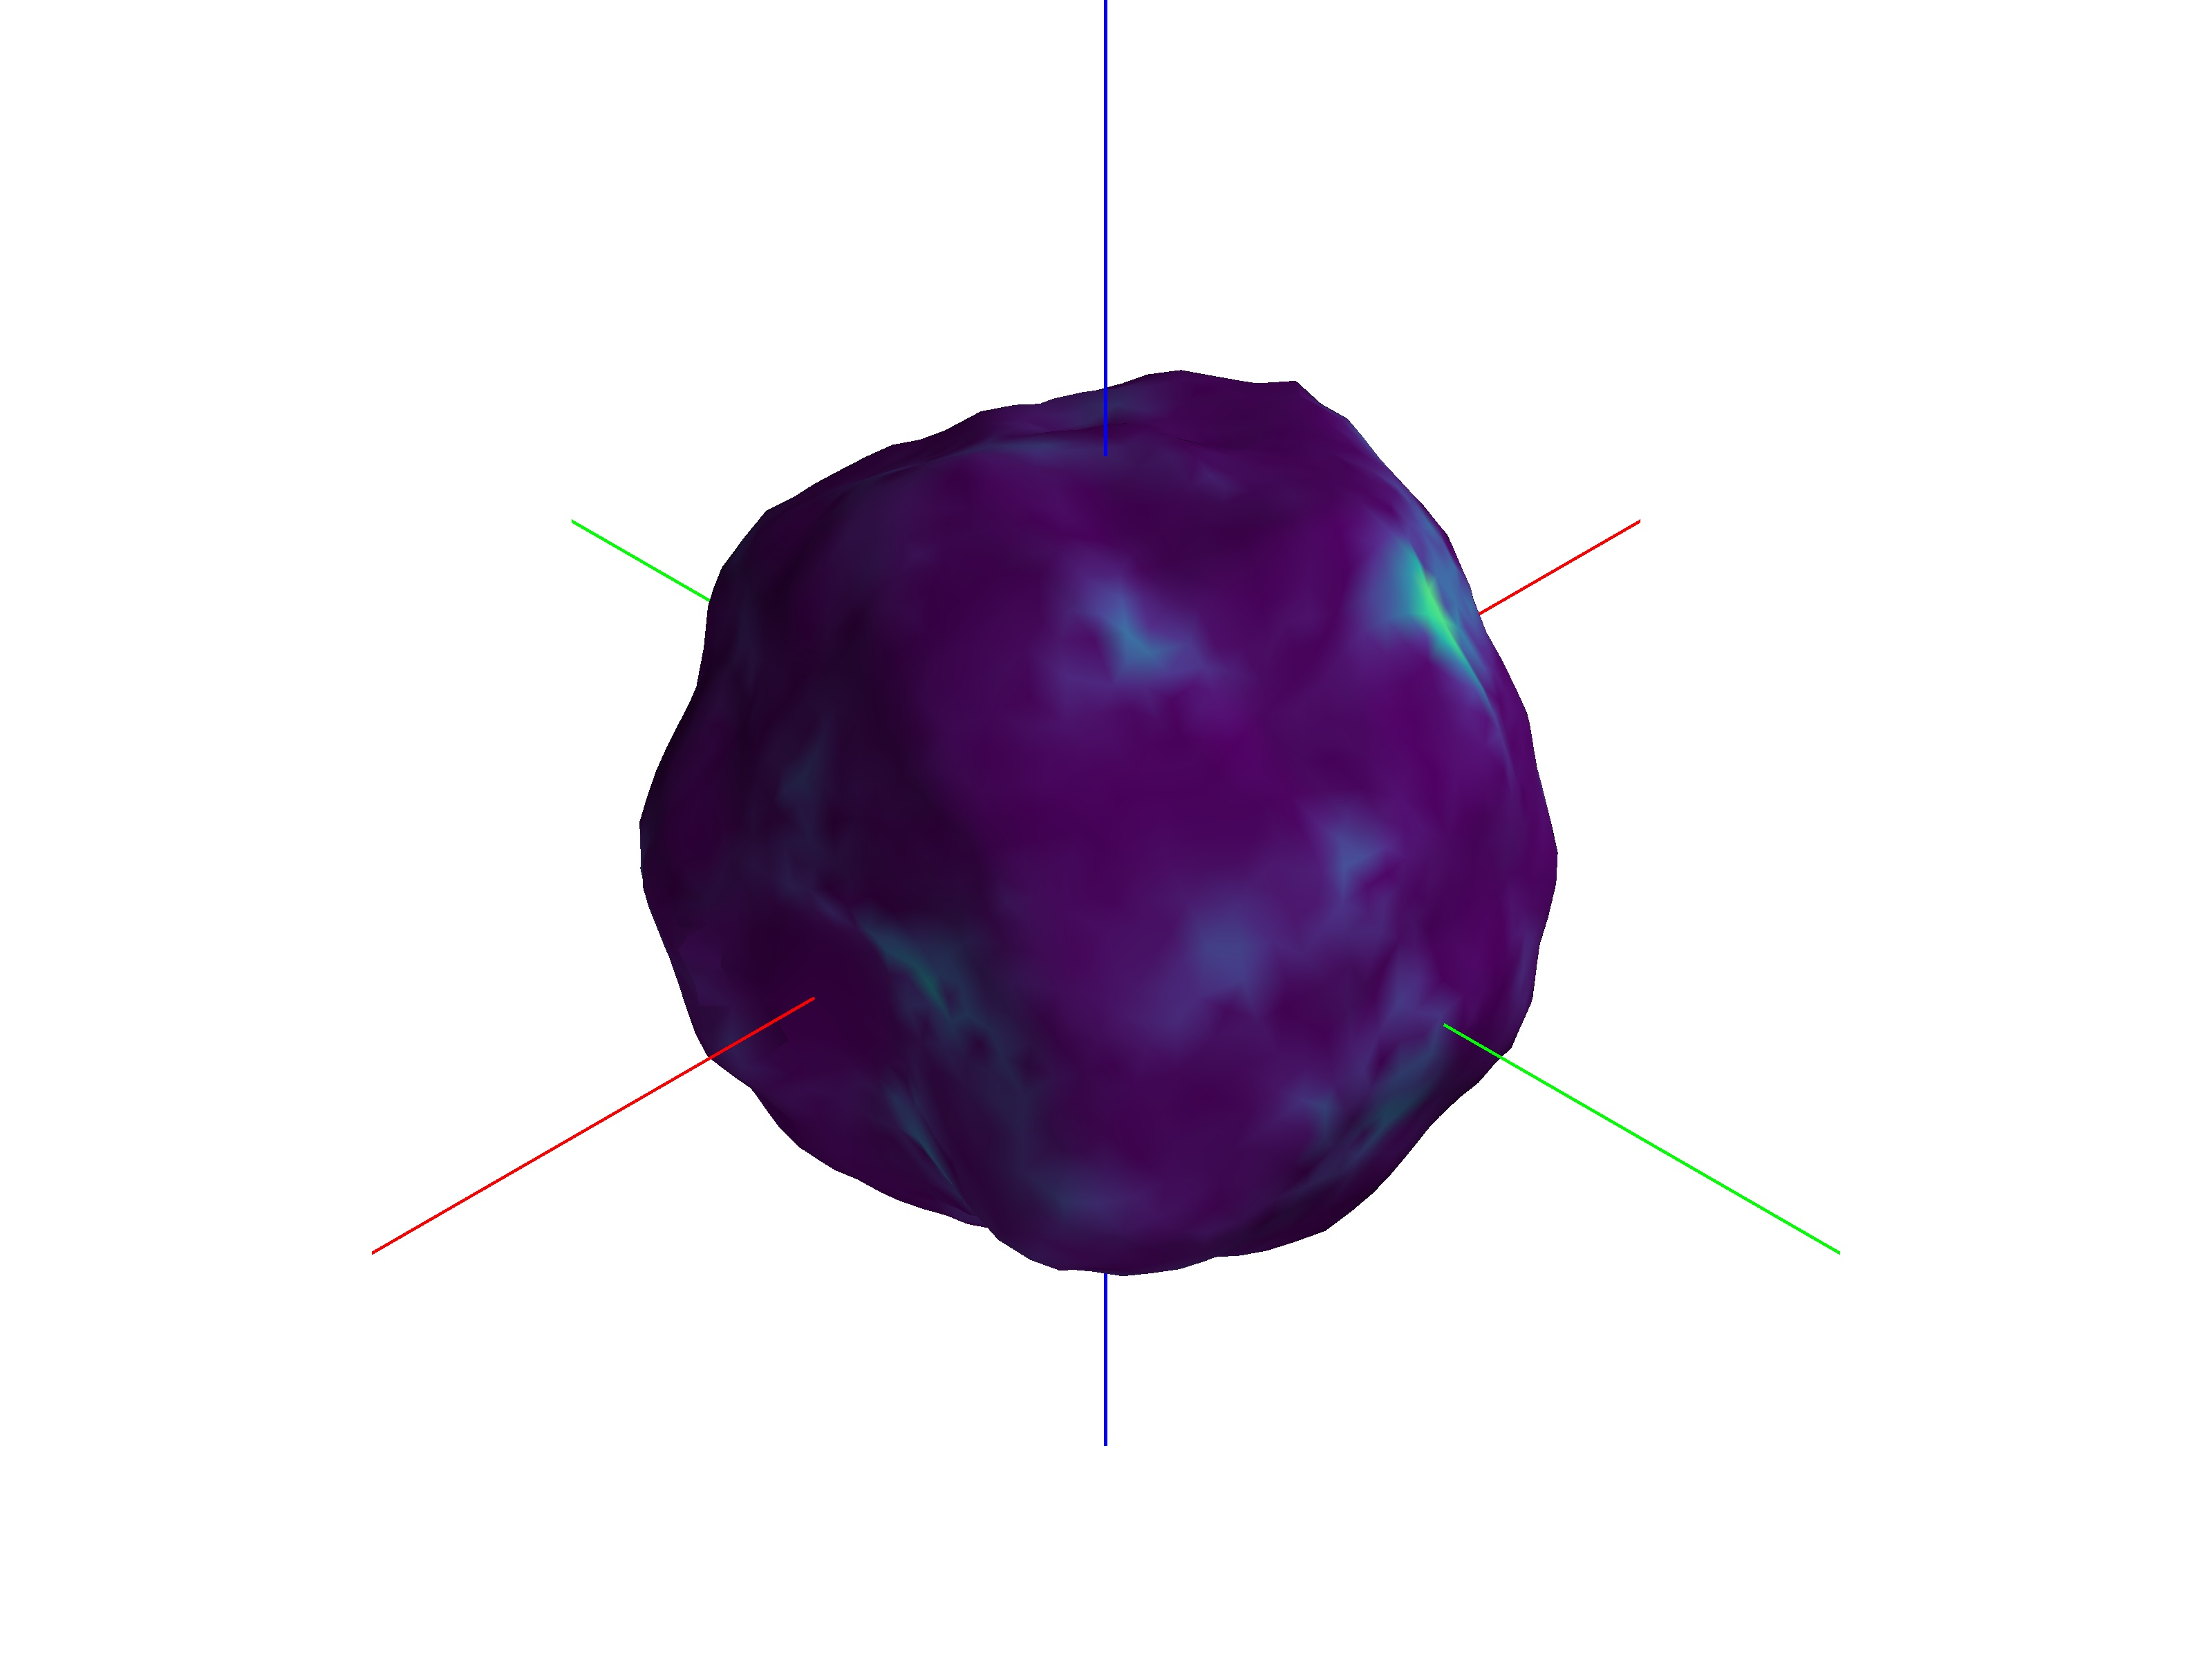
\includegraphics[trim={30cm 15cm 30cm 15cm},clip,height=0.25\textheight,width=0.3\textwidth,keepaspectratio]{figures/dynamic_exploration/52760/partial_weights_11249.jpg}}%
    \subcaptionbox{\SI{100}{\percent} of measurements\label{fig:52760_partial_weights_100}}{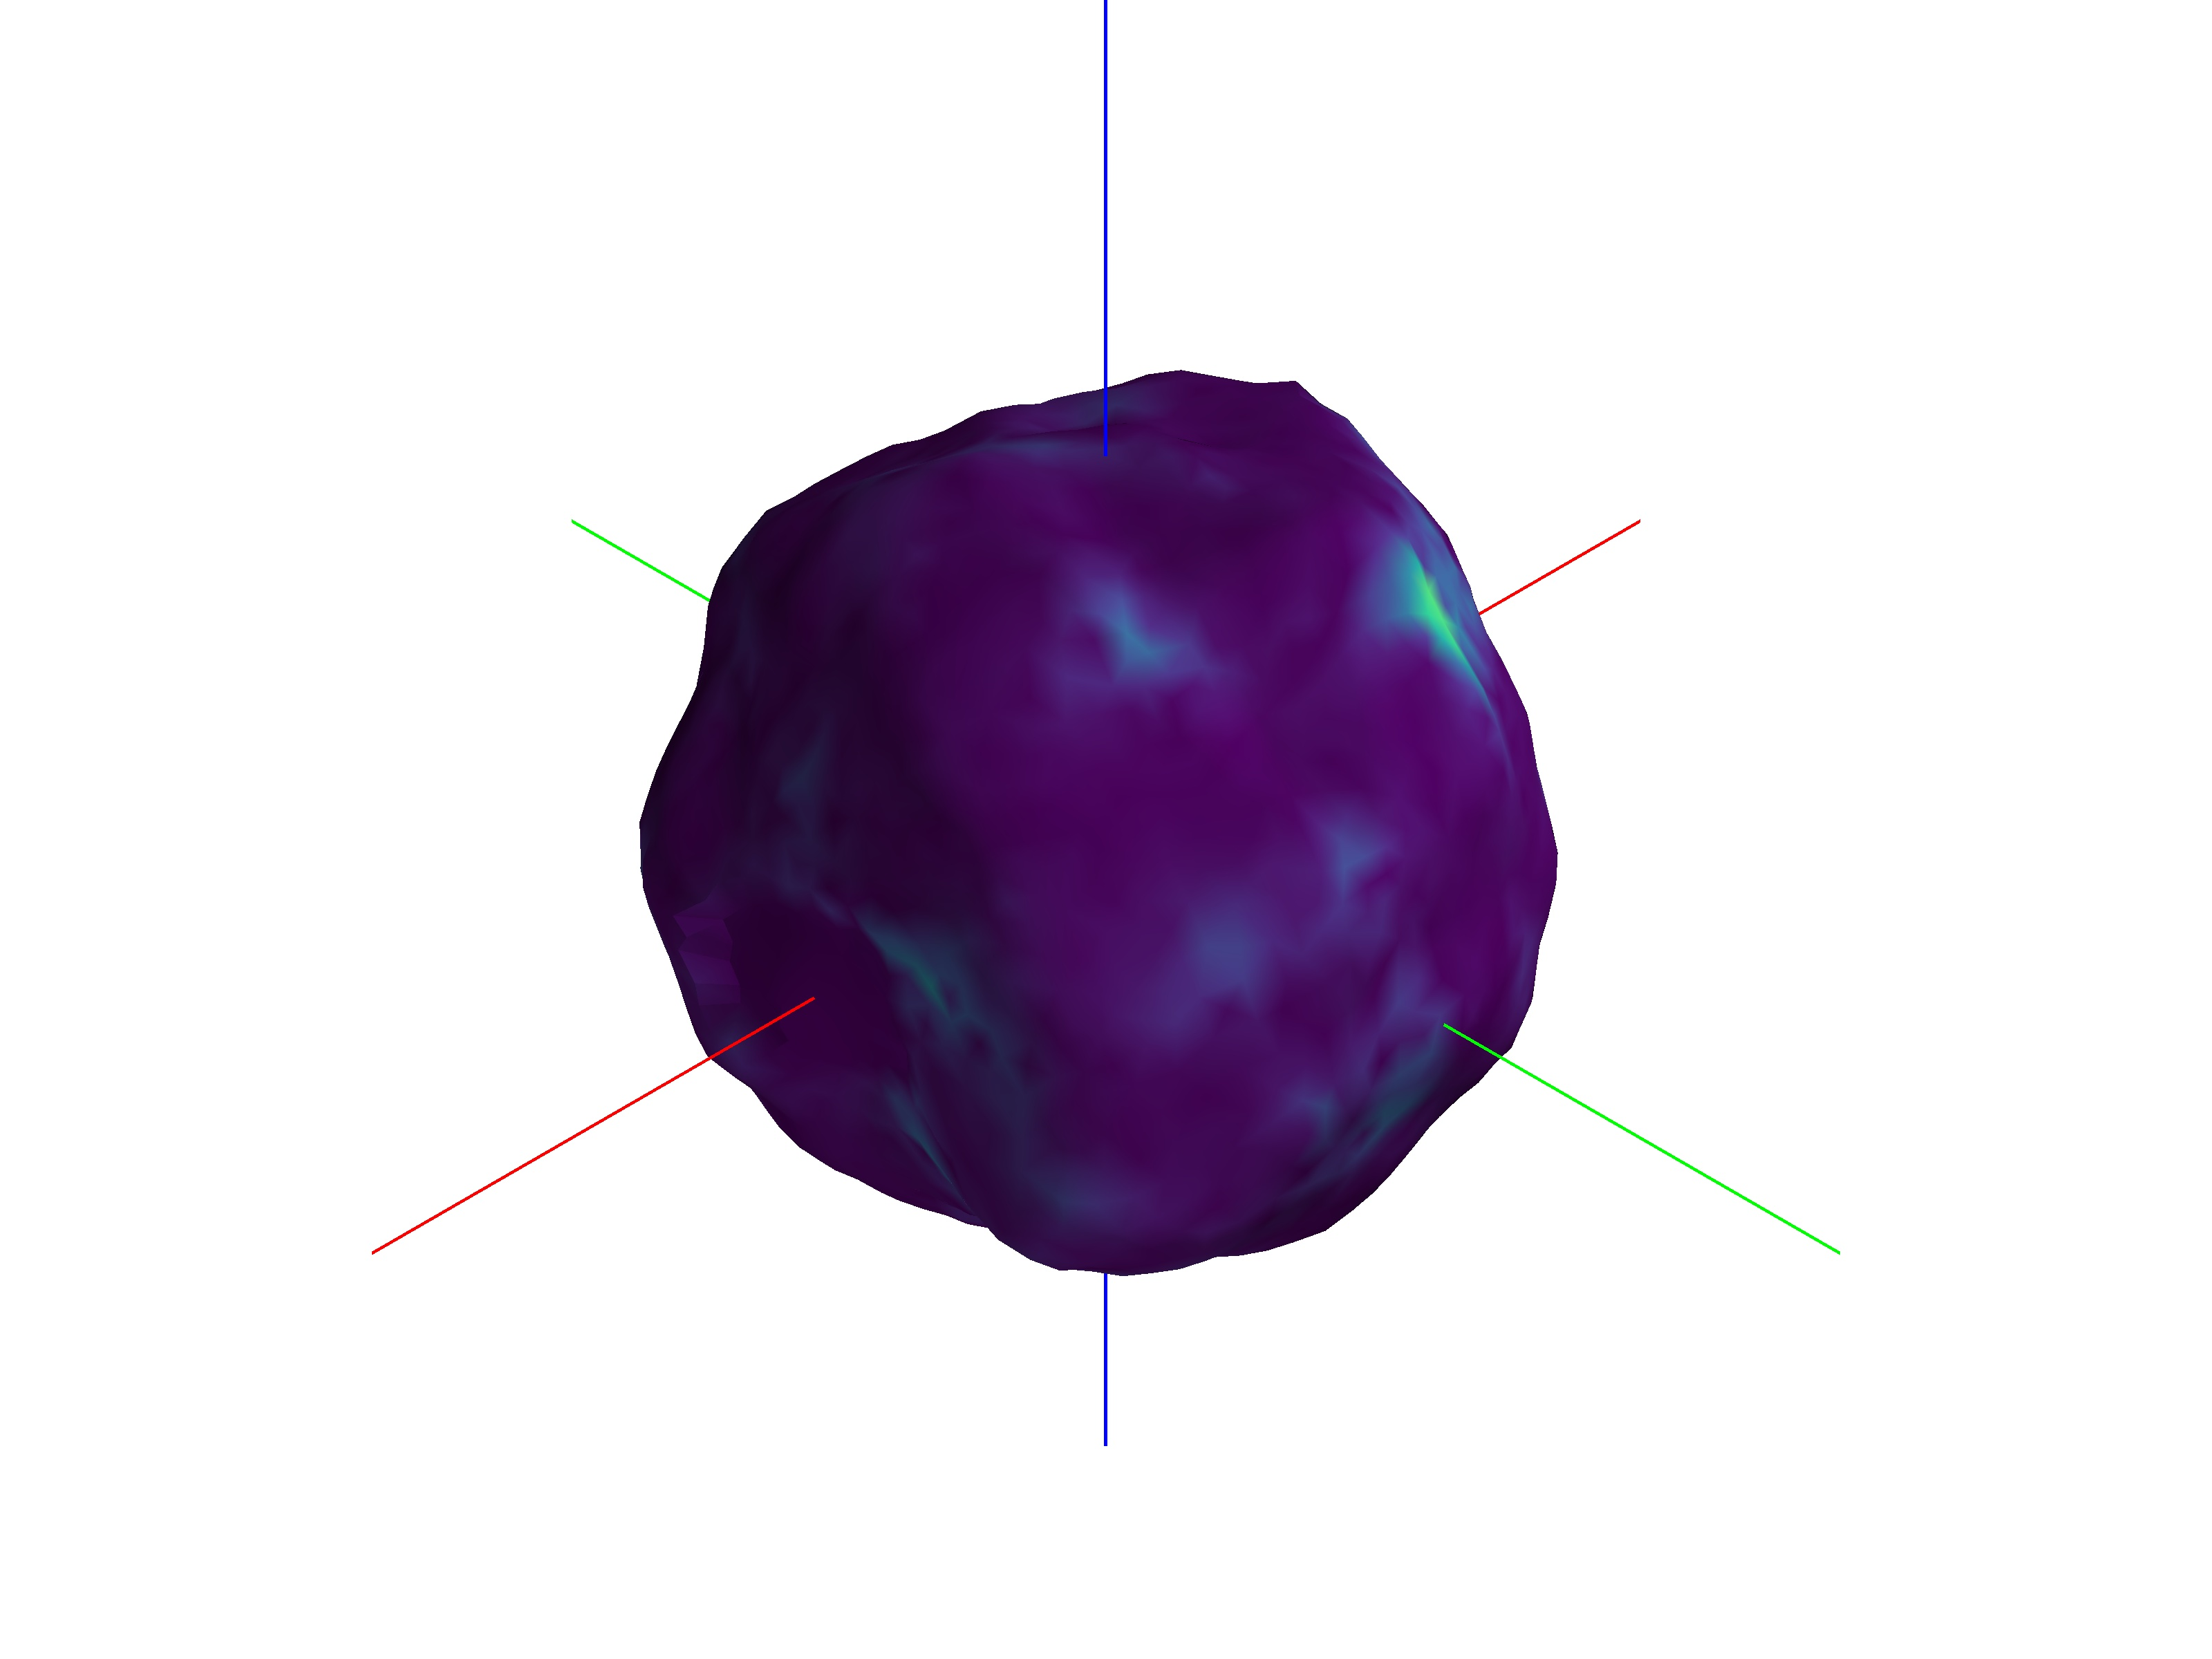
\includegraphics[trim={30cm 15cm 30cm 15cm},clip,height=0.25\textheight,width=0.3\textwidth,keepaspectratio]{figures/dynamic_exploration/52760/partial_weights_14998.jpg}}%
    \subcaptionbox{True Shape Model\label{fig:52760_weights_truth}}{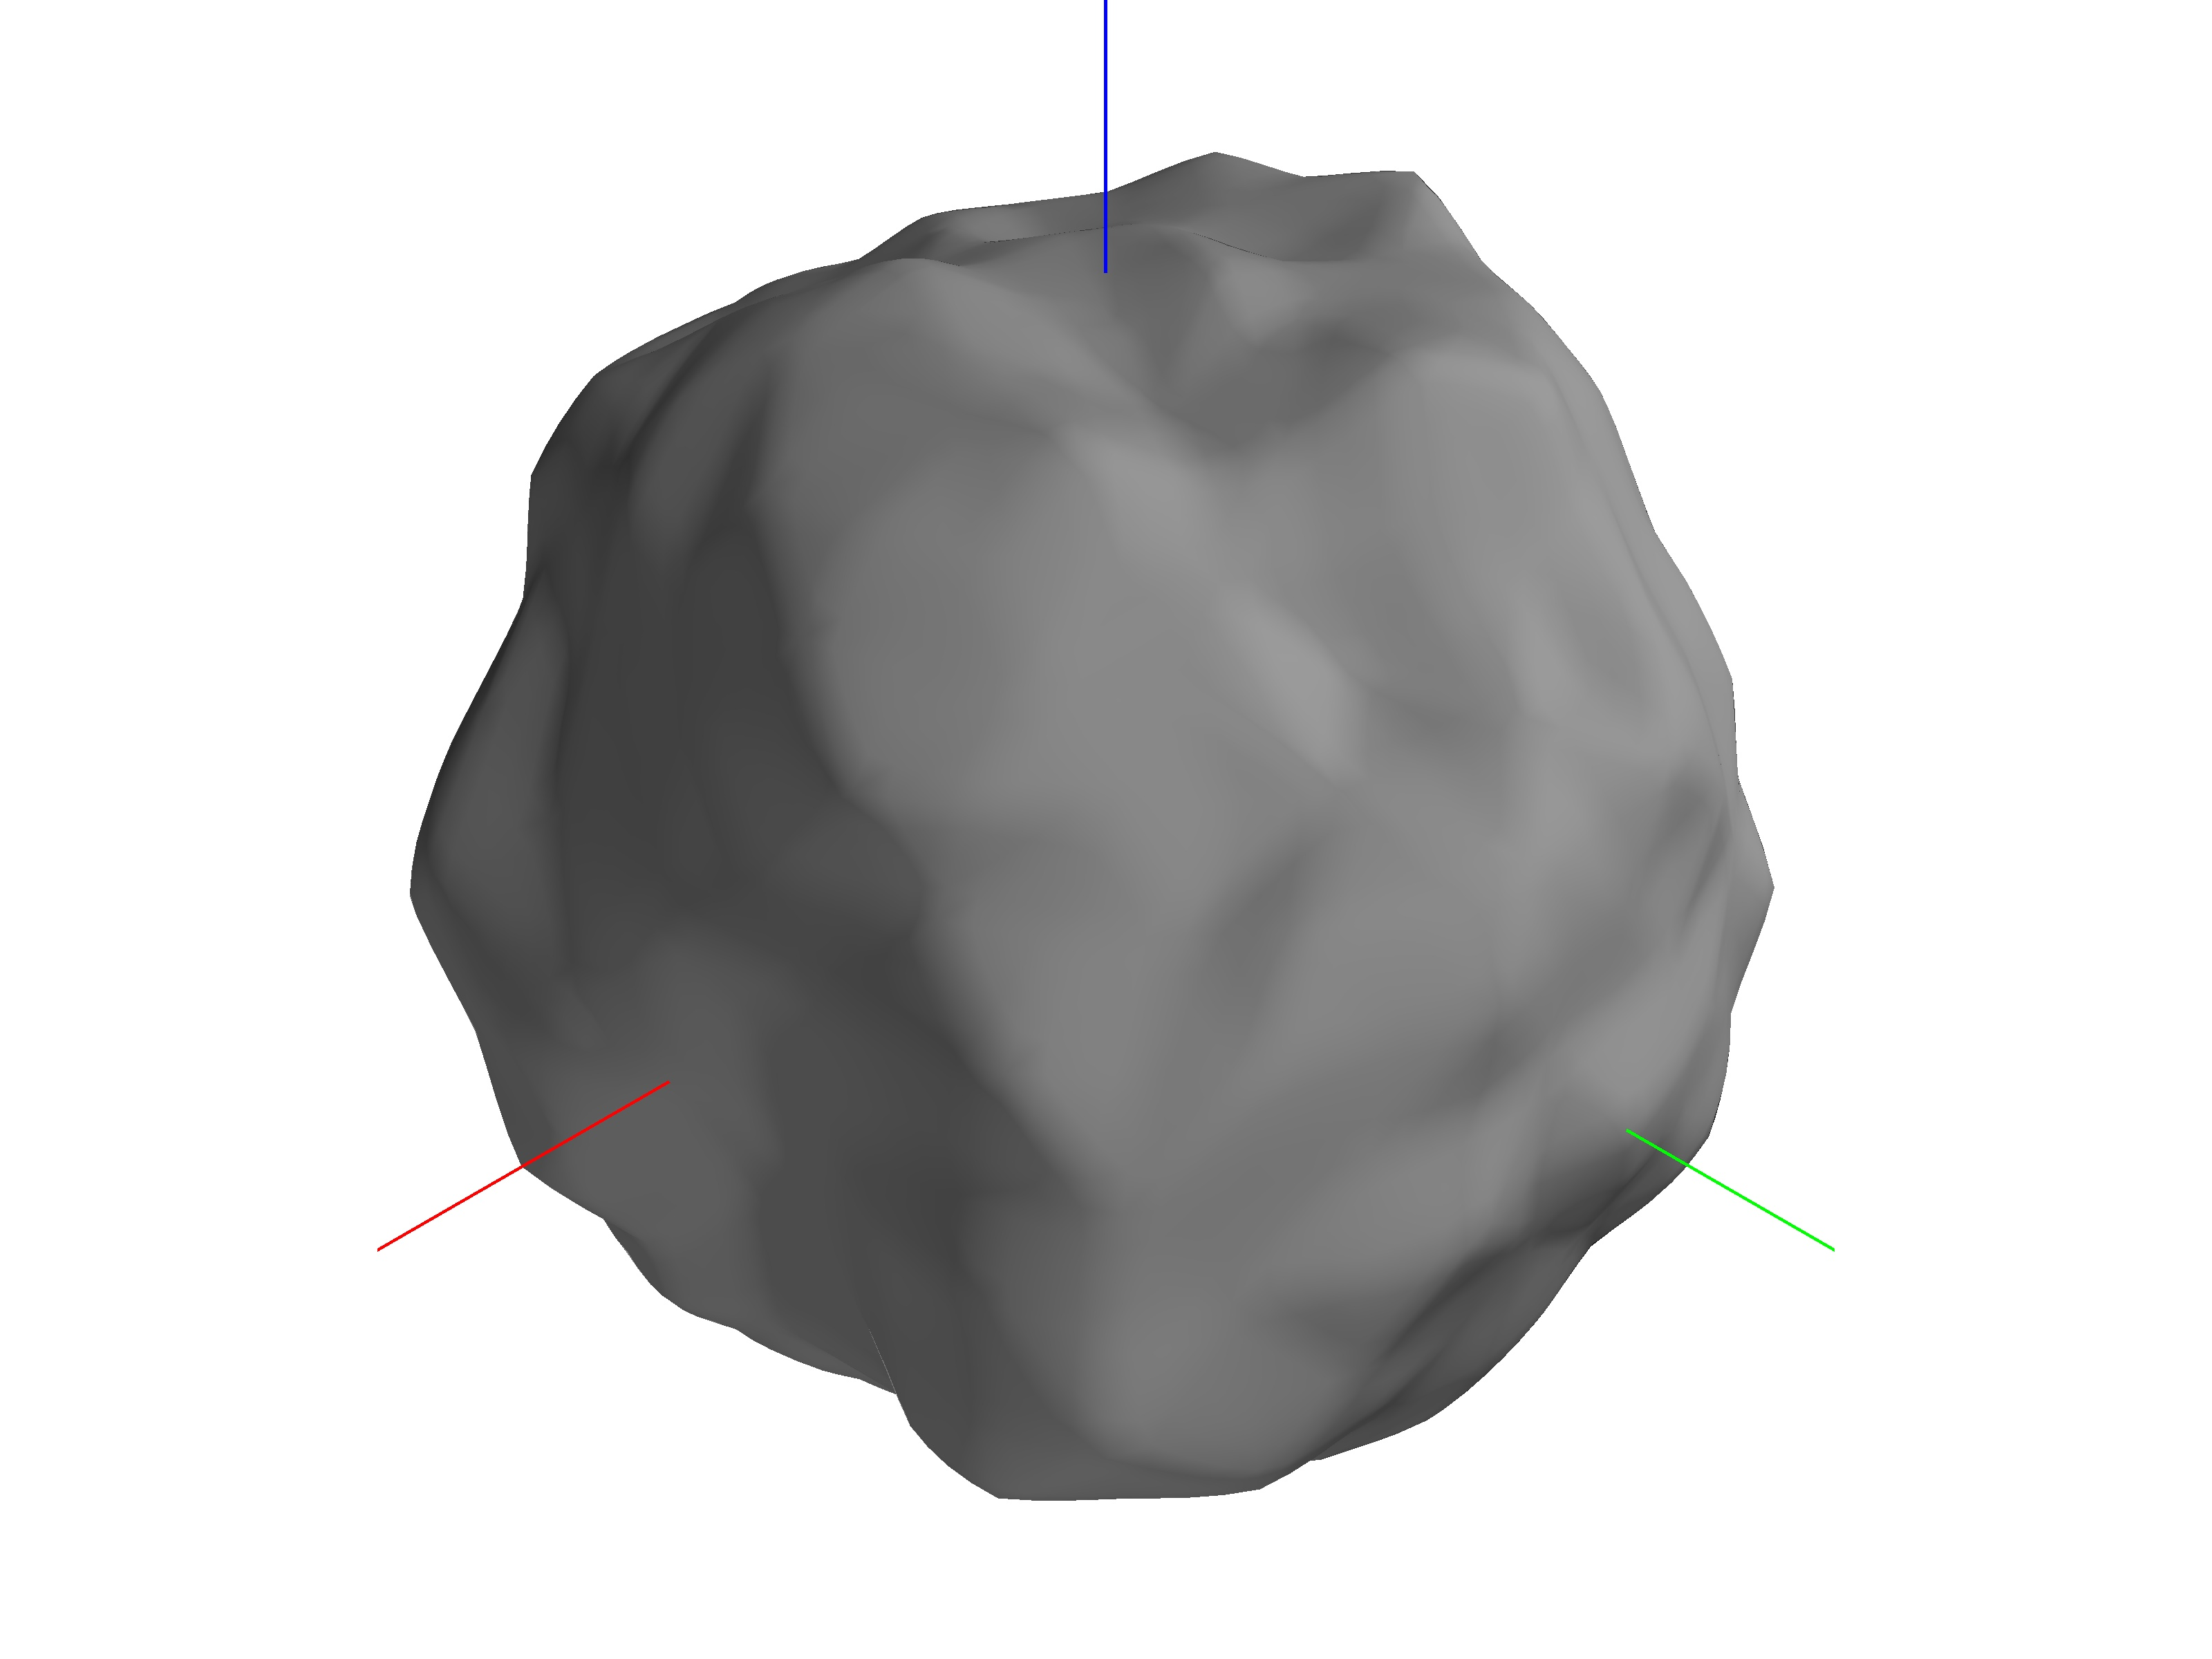
\includegraphics[trim={15cm 0cm 15cm 5cm},clip,height=0.25\textheight,width=0.3\textwidth,keepaspectratio]{figures/mesh_update/52760/truth.jpg}}
    \caption[Asteroid 52760 shape reconstruction with uncertainty]{Incremental reconstruction of asteroid 52760. The images colored according to the shape uncertainty. Areas of high uncertainty are in yellow while ares of low uncertainty are in purple.~\label{fig:52760_weights_reconstruction}}
\end{figure}

\paragraph{Asteroid 4769 Castalia Reconstruction}

Asteroid 4769 Castalia is a small near Earth asteroid of the Apollo group.
In addition, it is classified as a potentially hazardous object with a closed approach distance of less than \SI{0.05}{\astronomicalunit}.
Castalia was discovered in \num{1989} and is the first asteroid to be modeled using radar imagery~\cite{hudson1994}.
Castalia is composed of two distinct lobes suggesting that it is a contact binary of two smaller objects held together by their mutual gravity.
\Cref{fig:castalia_weights_reconstruction} show the shape reconstruction at several discrete points during the simulation.
In addition~\cref{fig:castalia_weights_reconstruction} displays the vertex uncertainty \( w_i \) as a colormap on the surface. 
Areas of high uncertainty are denoted in yellow while areas of low uncertainty are in purple/blue.
Within \SI{50}{\percent} of the simulation span the spacecraft is able to achieve an accurate estimate of the true shape of Castalia.

\begin{figure}[htbp]
    \centering
    \subcaptionbox{Initial Shape Estimate\label{fig:castalia_partial_weights_0}}{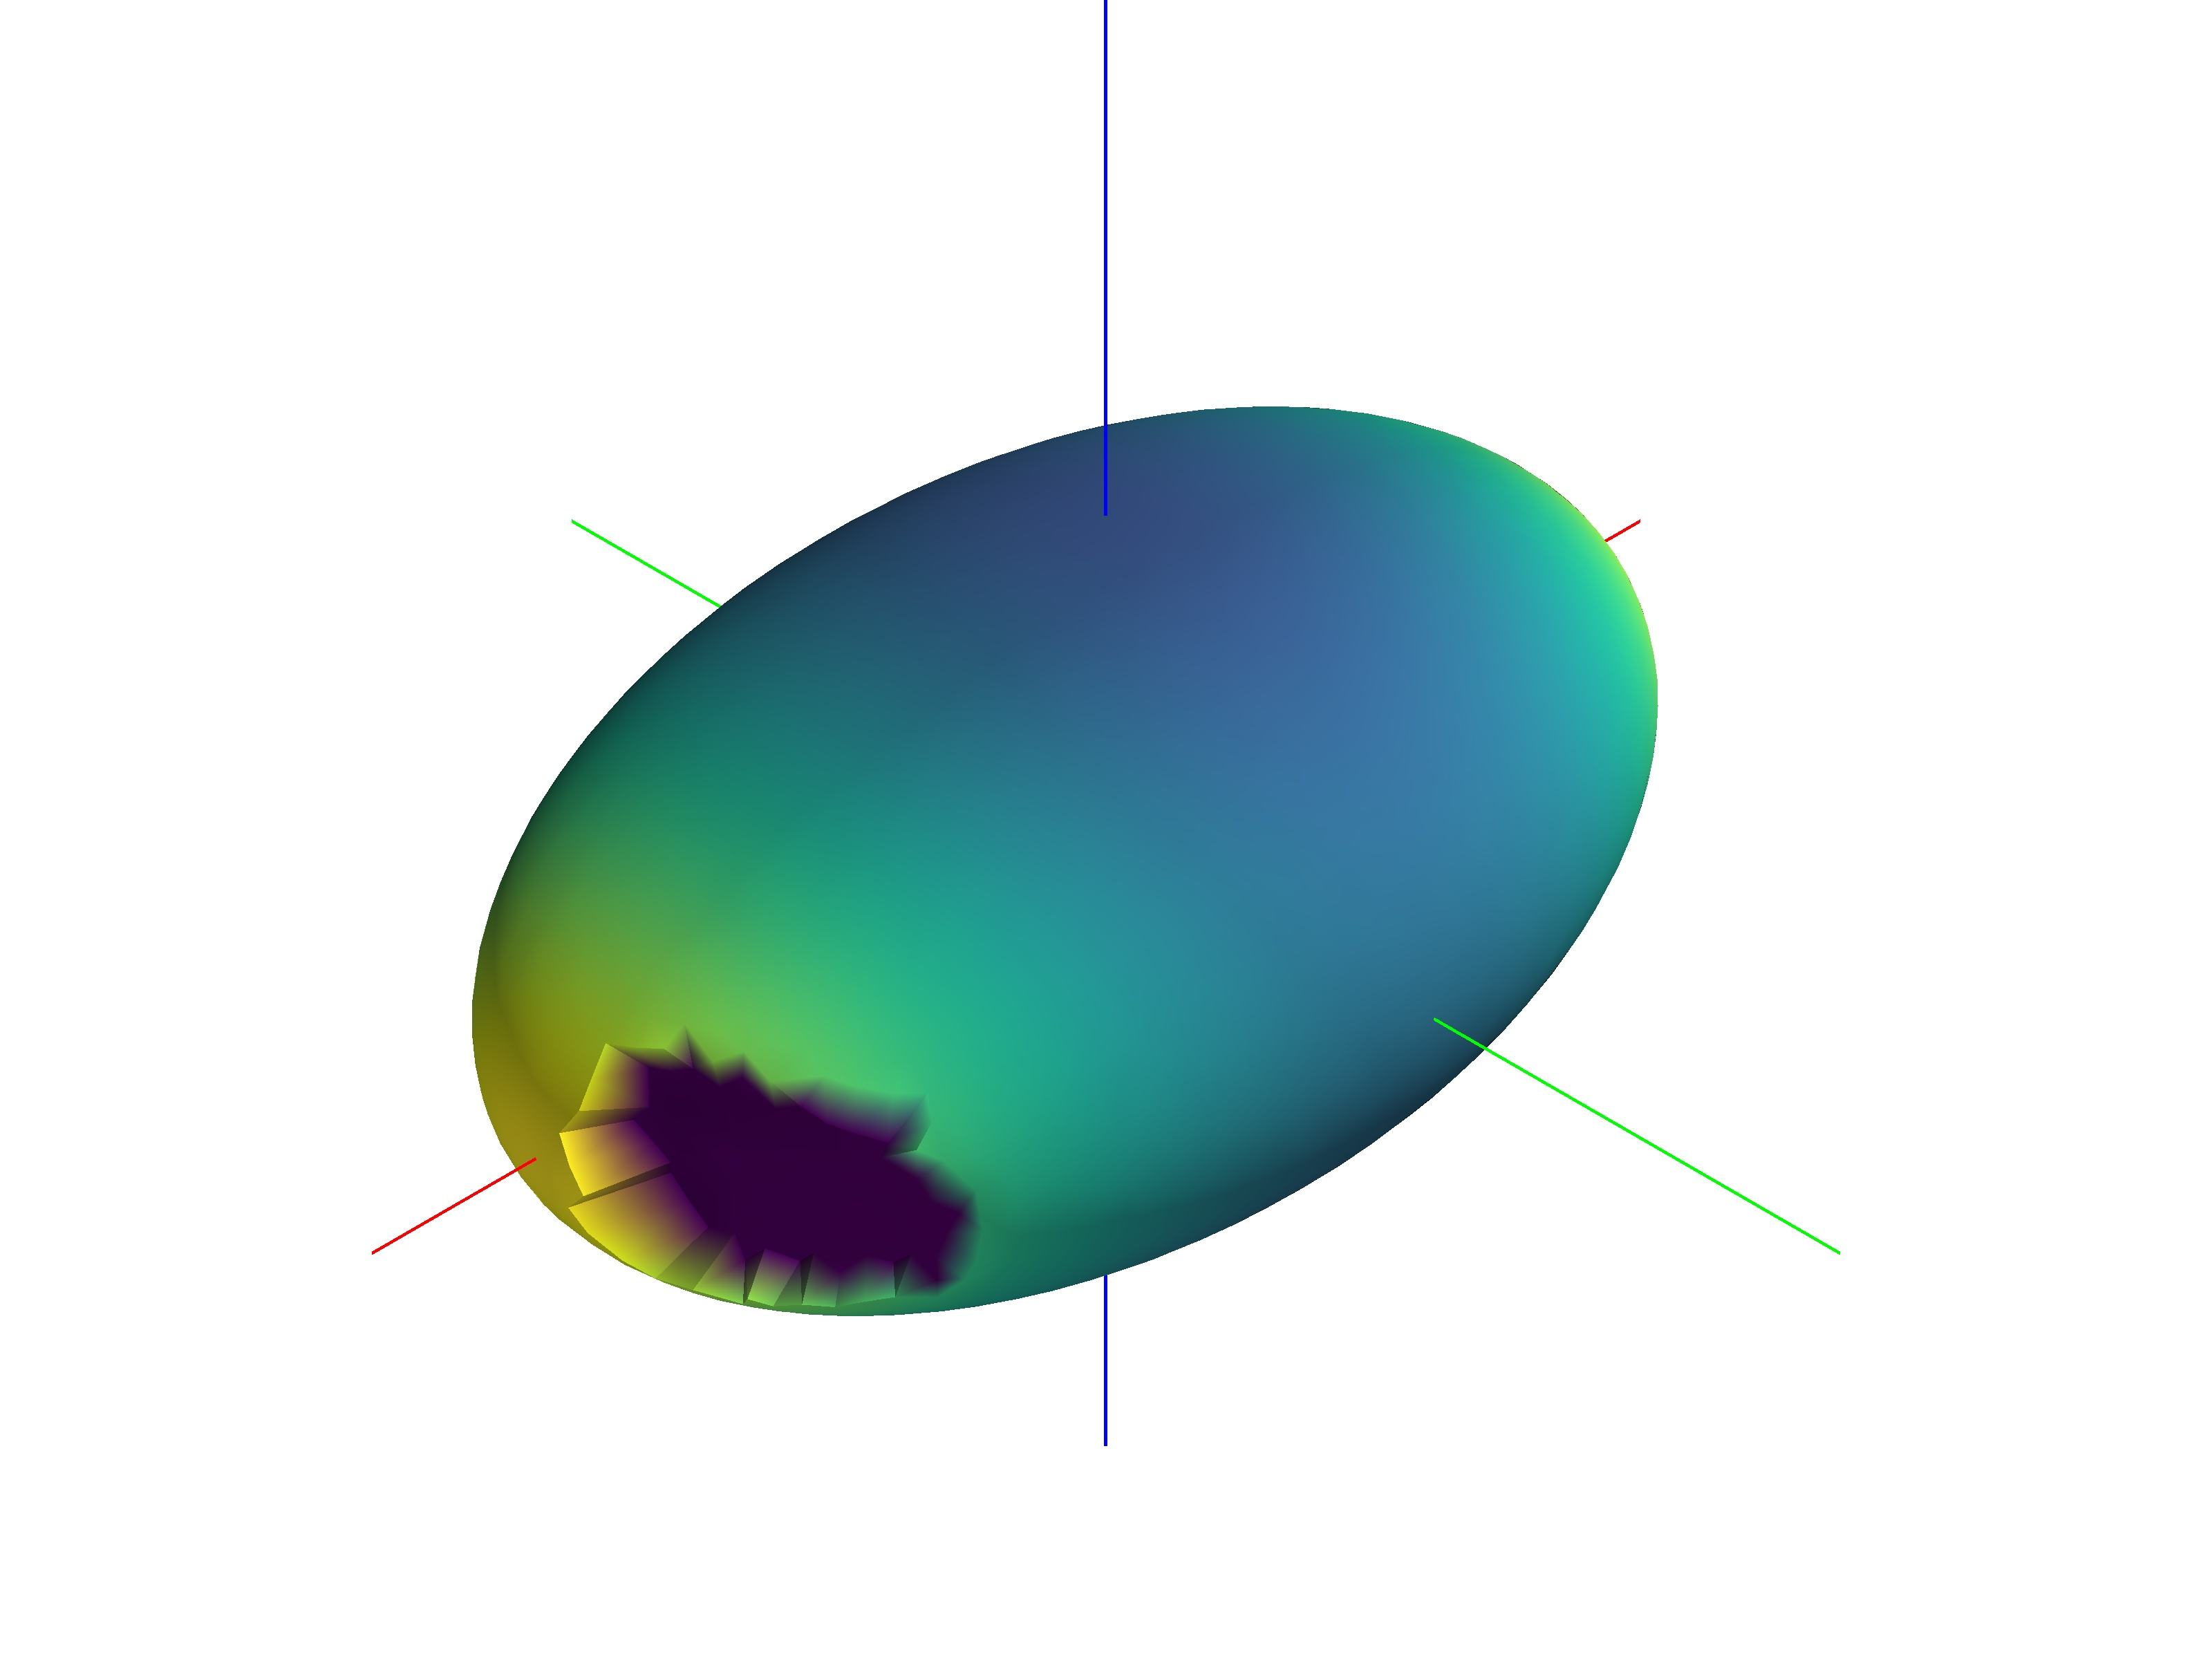
\includegraphics[trim={15cm 10cm 15cm 10cm},clip,height=0.5\textheight,width=0.3\textwidth,keepaspectratio]{figures/dynamic_exploration/castalia/partial_weights_1.jpg}}%
    \subcaptionbox{\SI{25}{\percent} of measurements added\label{fig:castalia_partial_weights_25}}{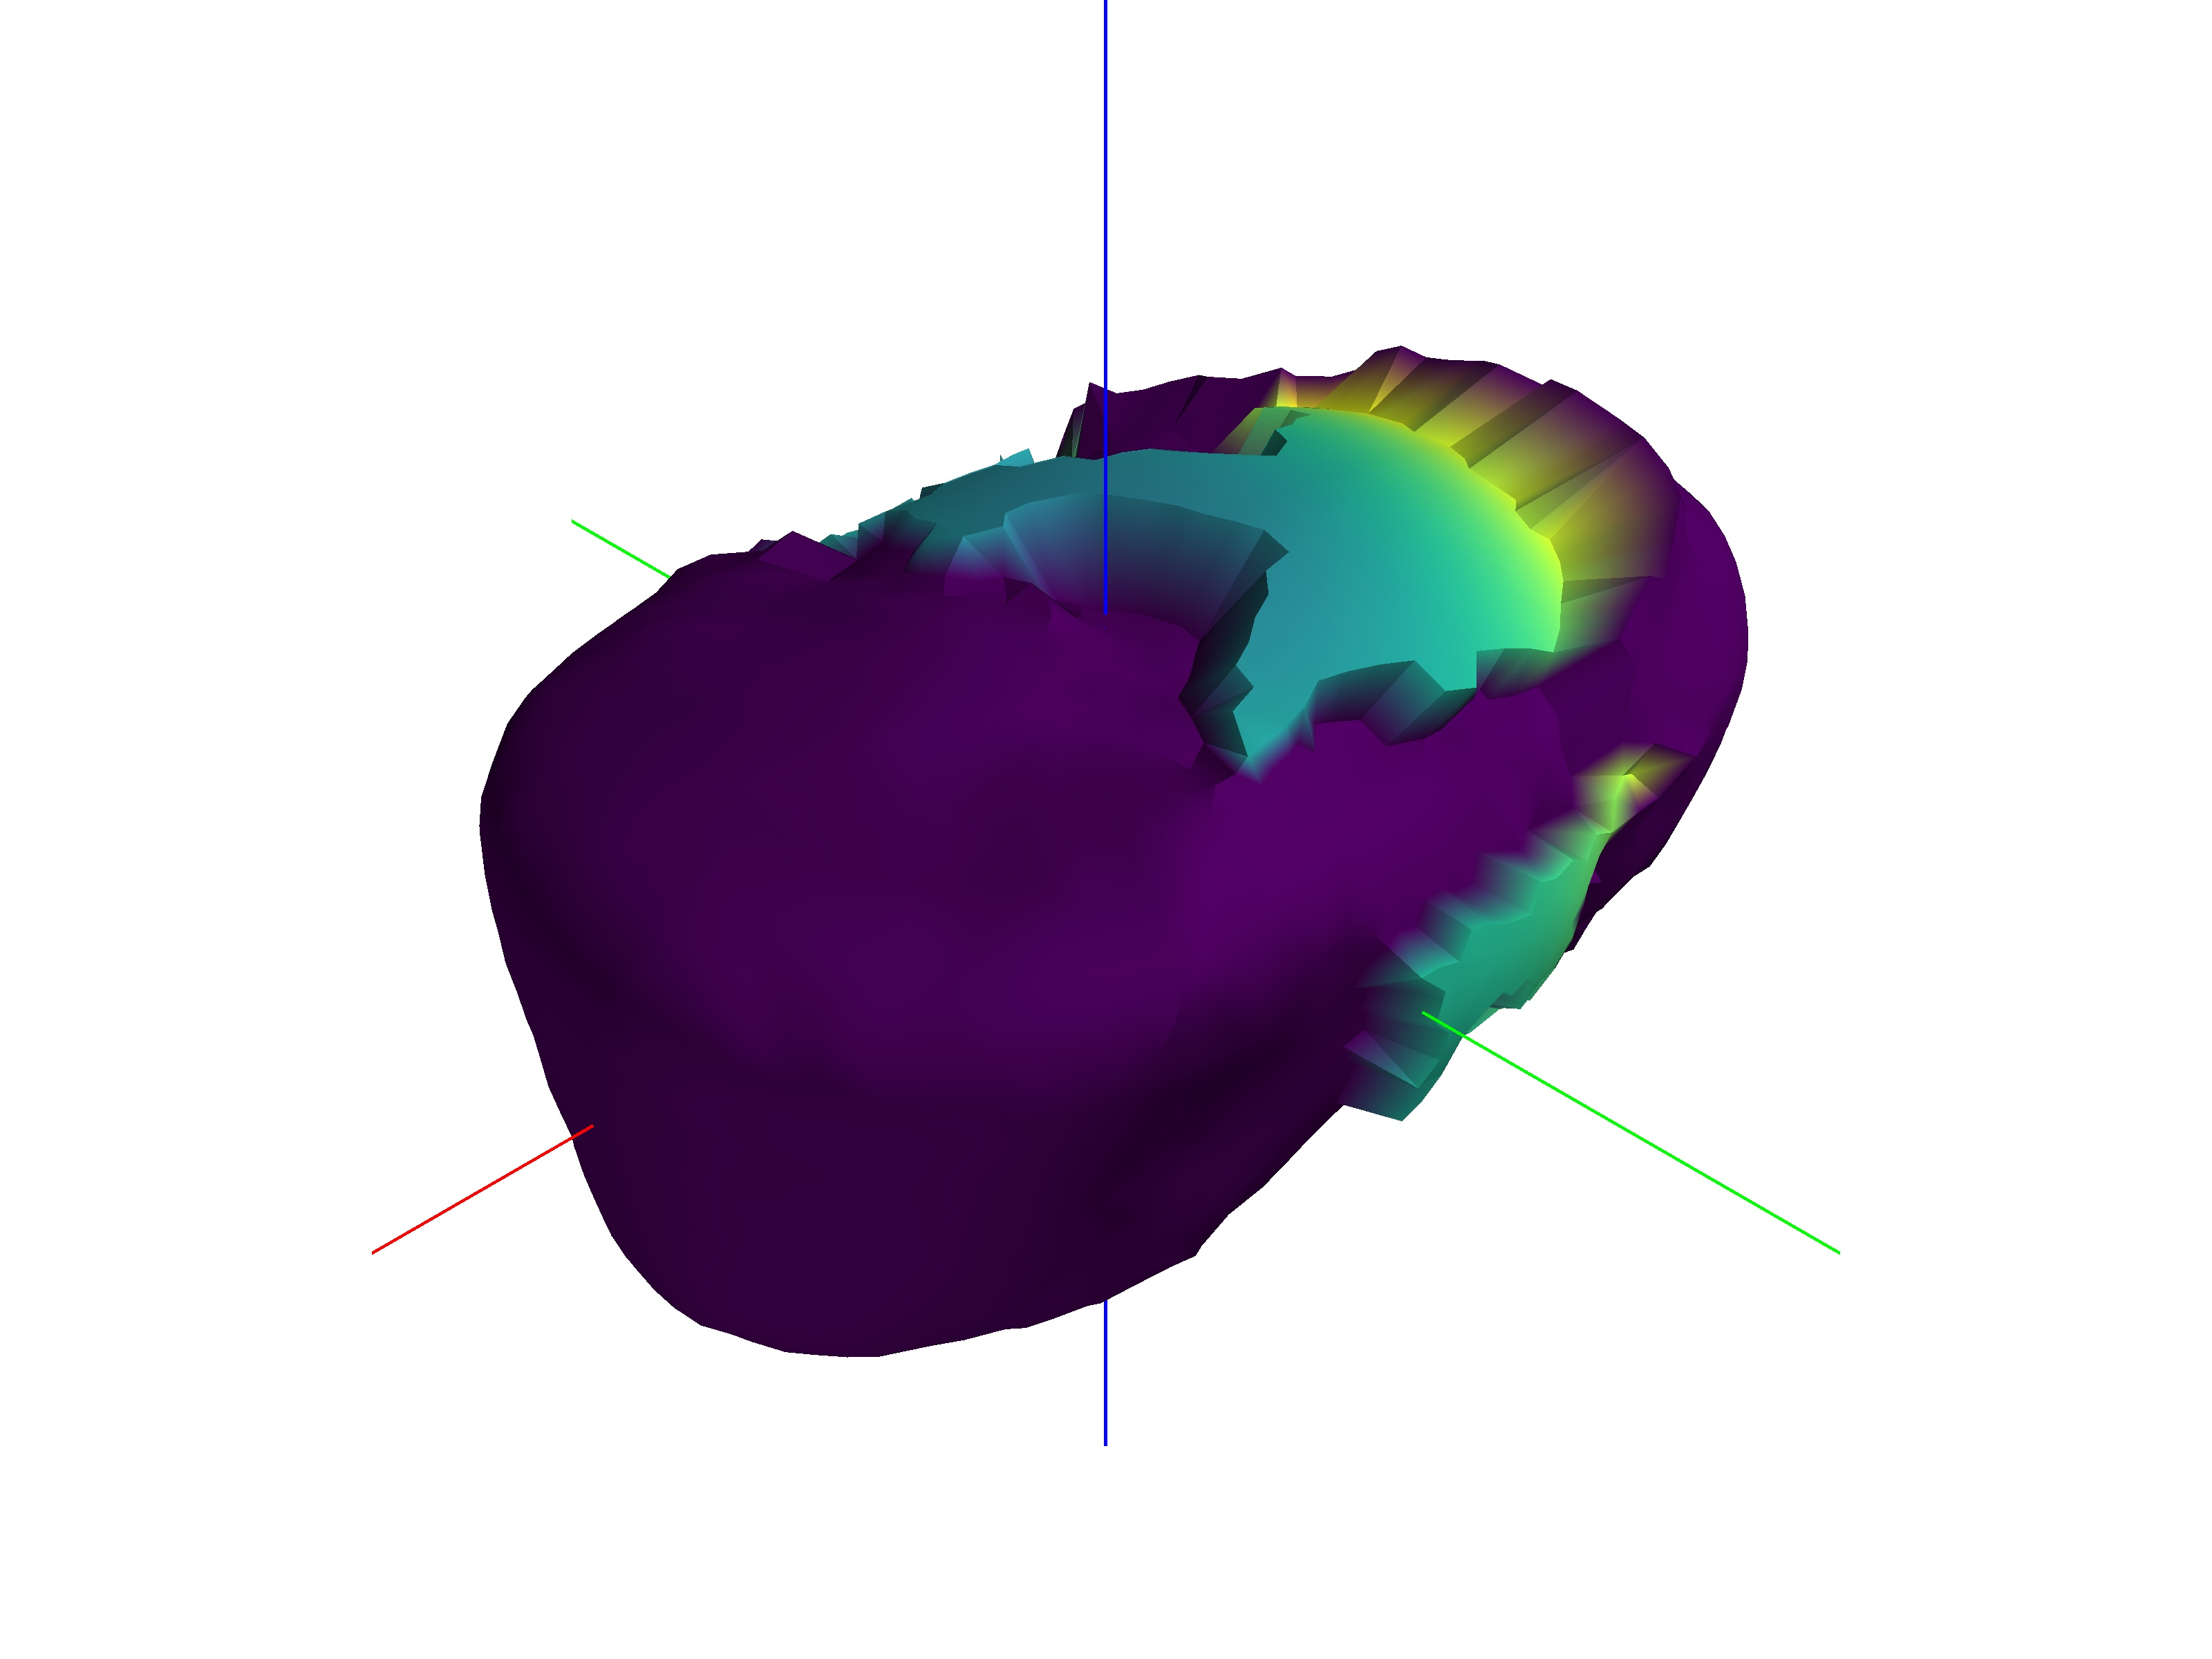
\includegraphics[trim={15cm 10cm 15cm 10cm},clip,height=0.5\textheight,width=0.3\textwidth,keepaspectratio]{figures/dynamic_exploration/castalia/partial_weights_3749.jpg}}%
    \subcaptionbox{\SI{50}{\percent} of measurements added\label{fig:castalia_partial_weights_50}}{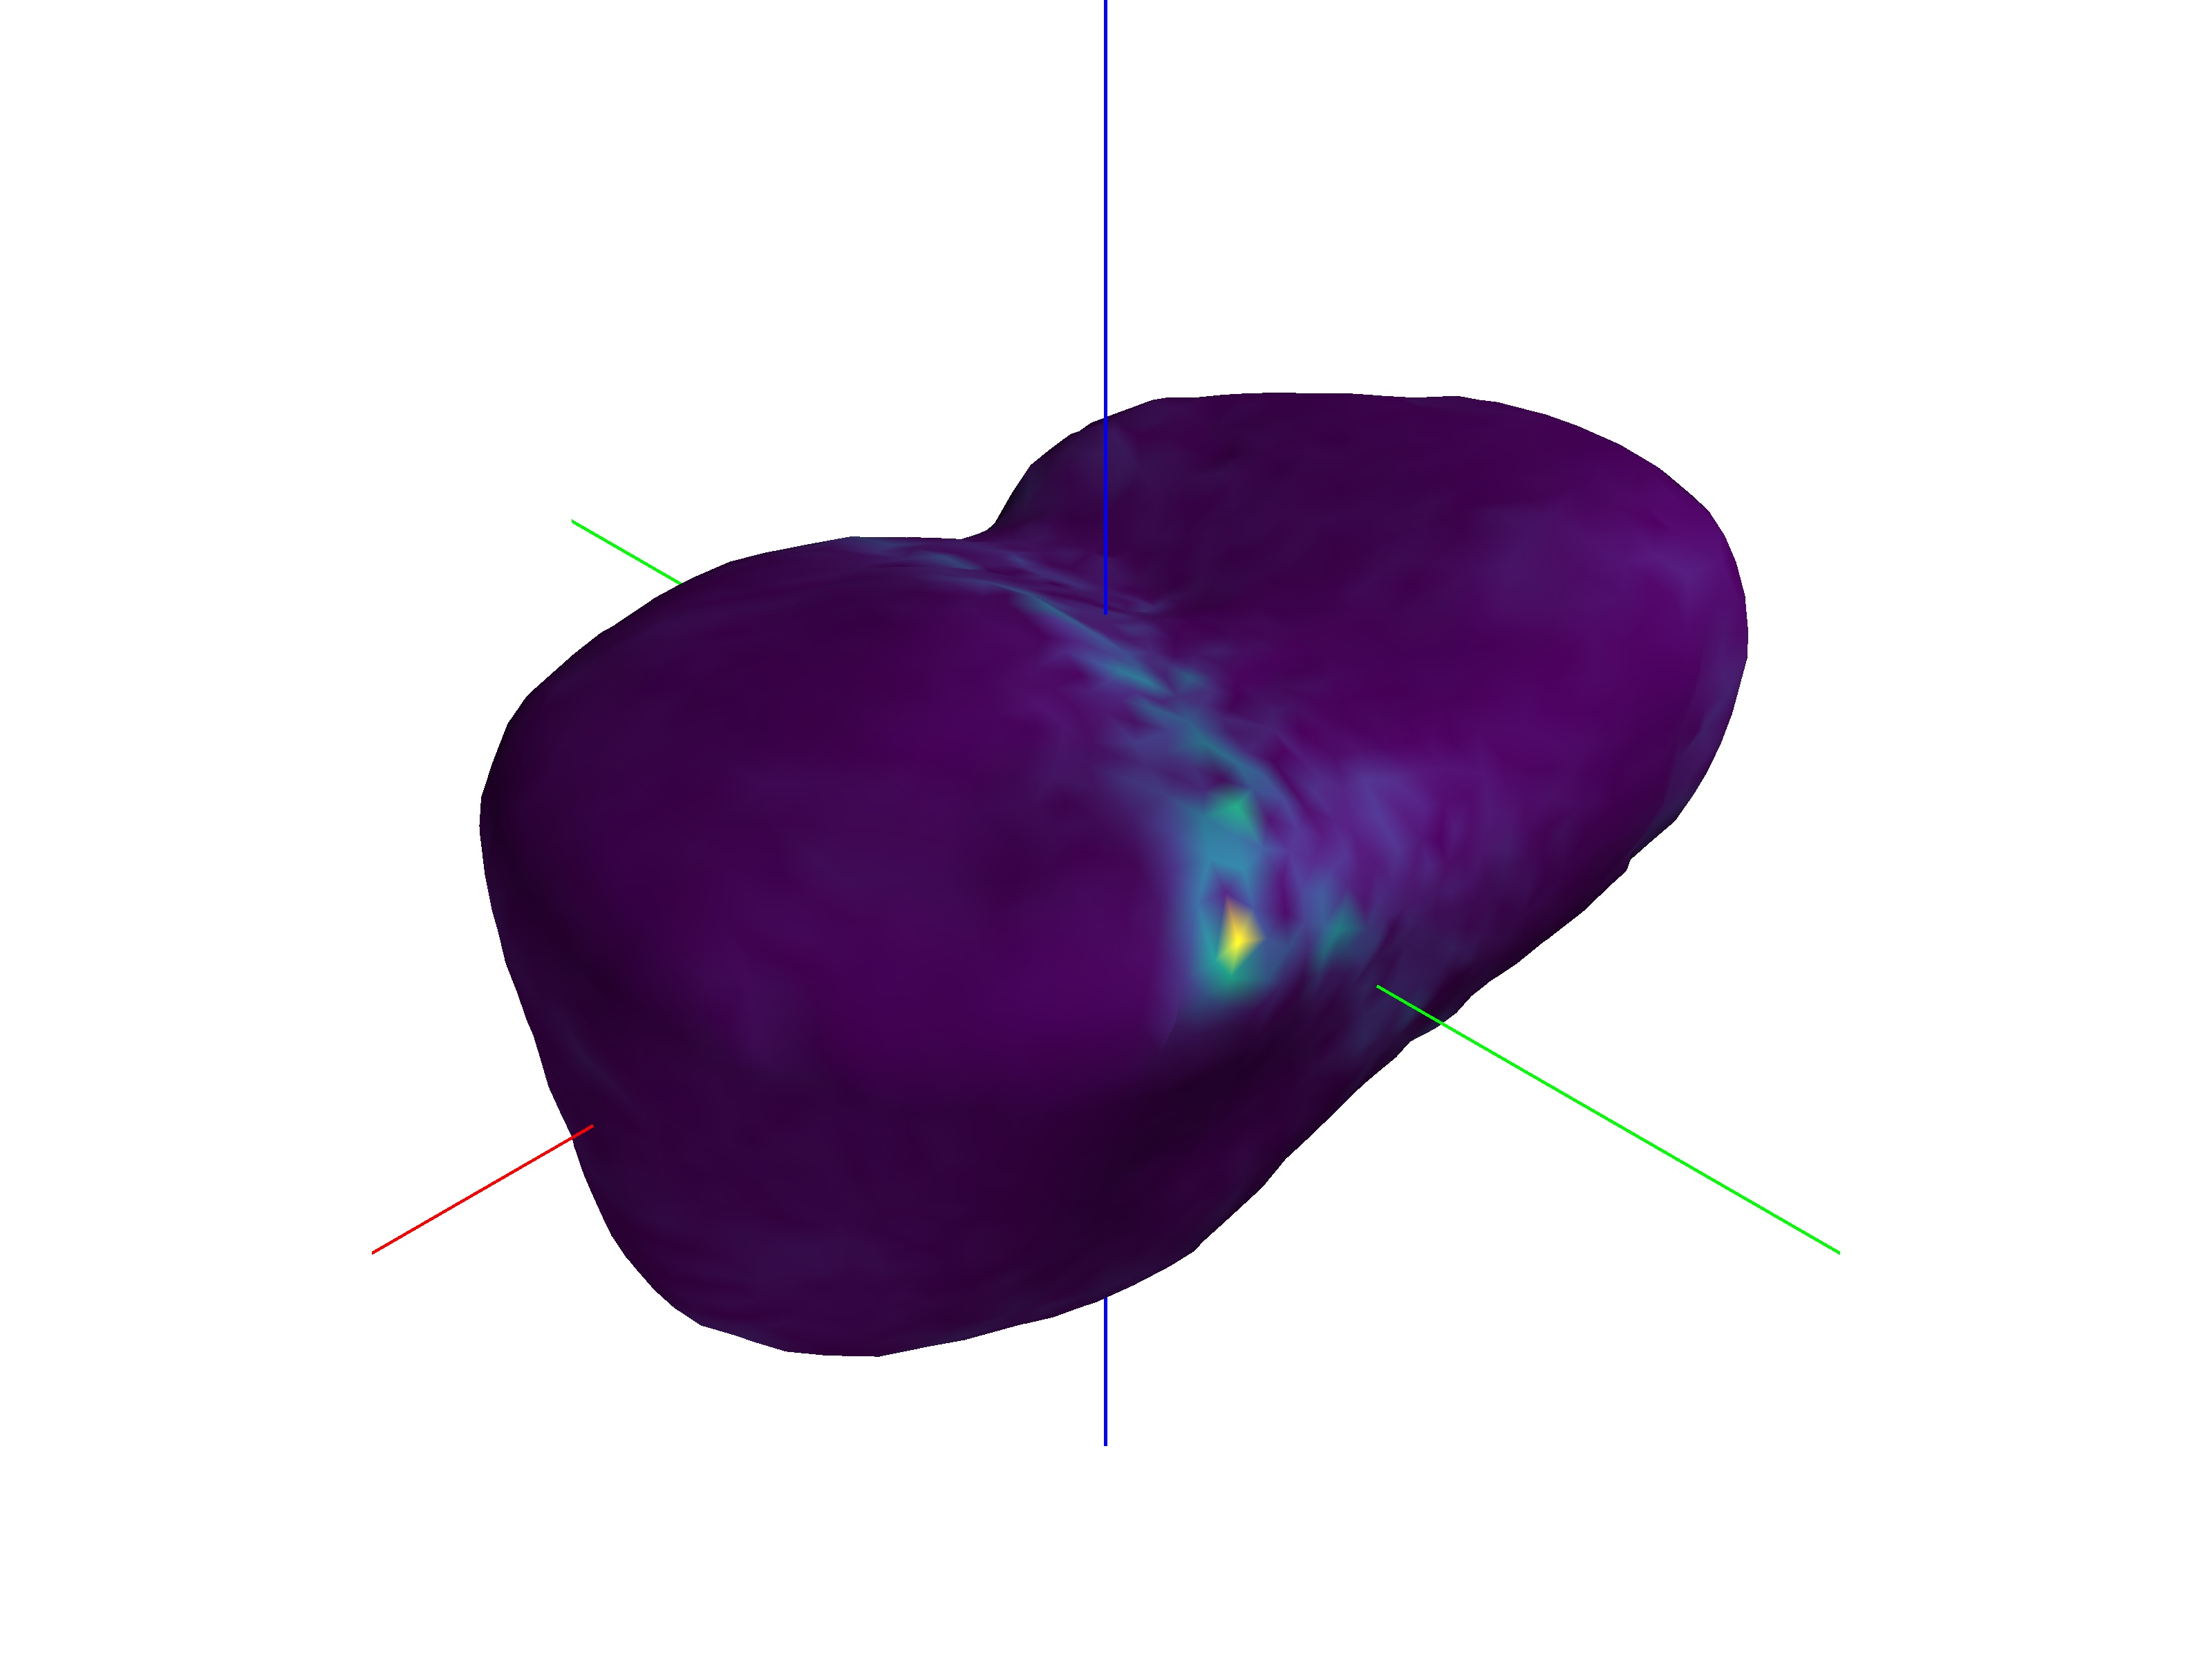
\includegraphics[trim={15cm 10cm 15cm 10cm},clip,height=0.5\textheight,width=0.3\textwidth,keepaspectratio]{figures/dynamic_exploration/castalia/partial_weights_7499.jpg}}

    \subcaptionbox{\SI{75}{\percent} of measurements added\label{fig:castalia_partial_weights_75}}{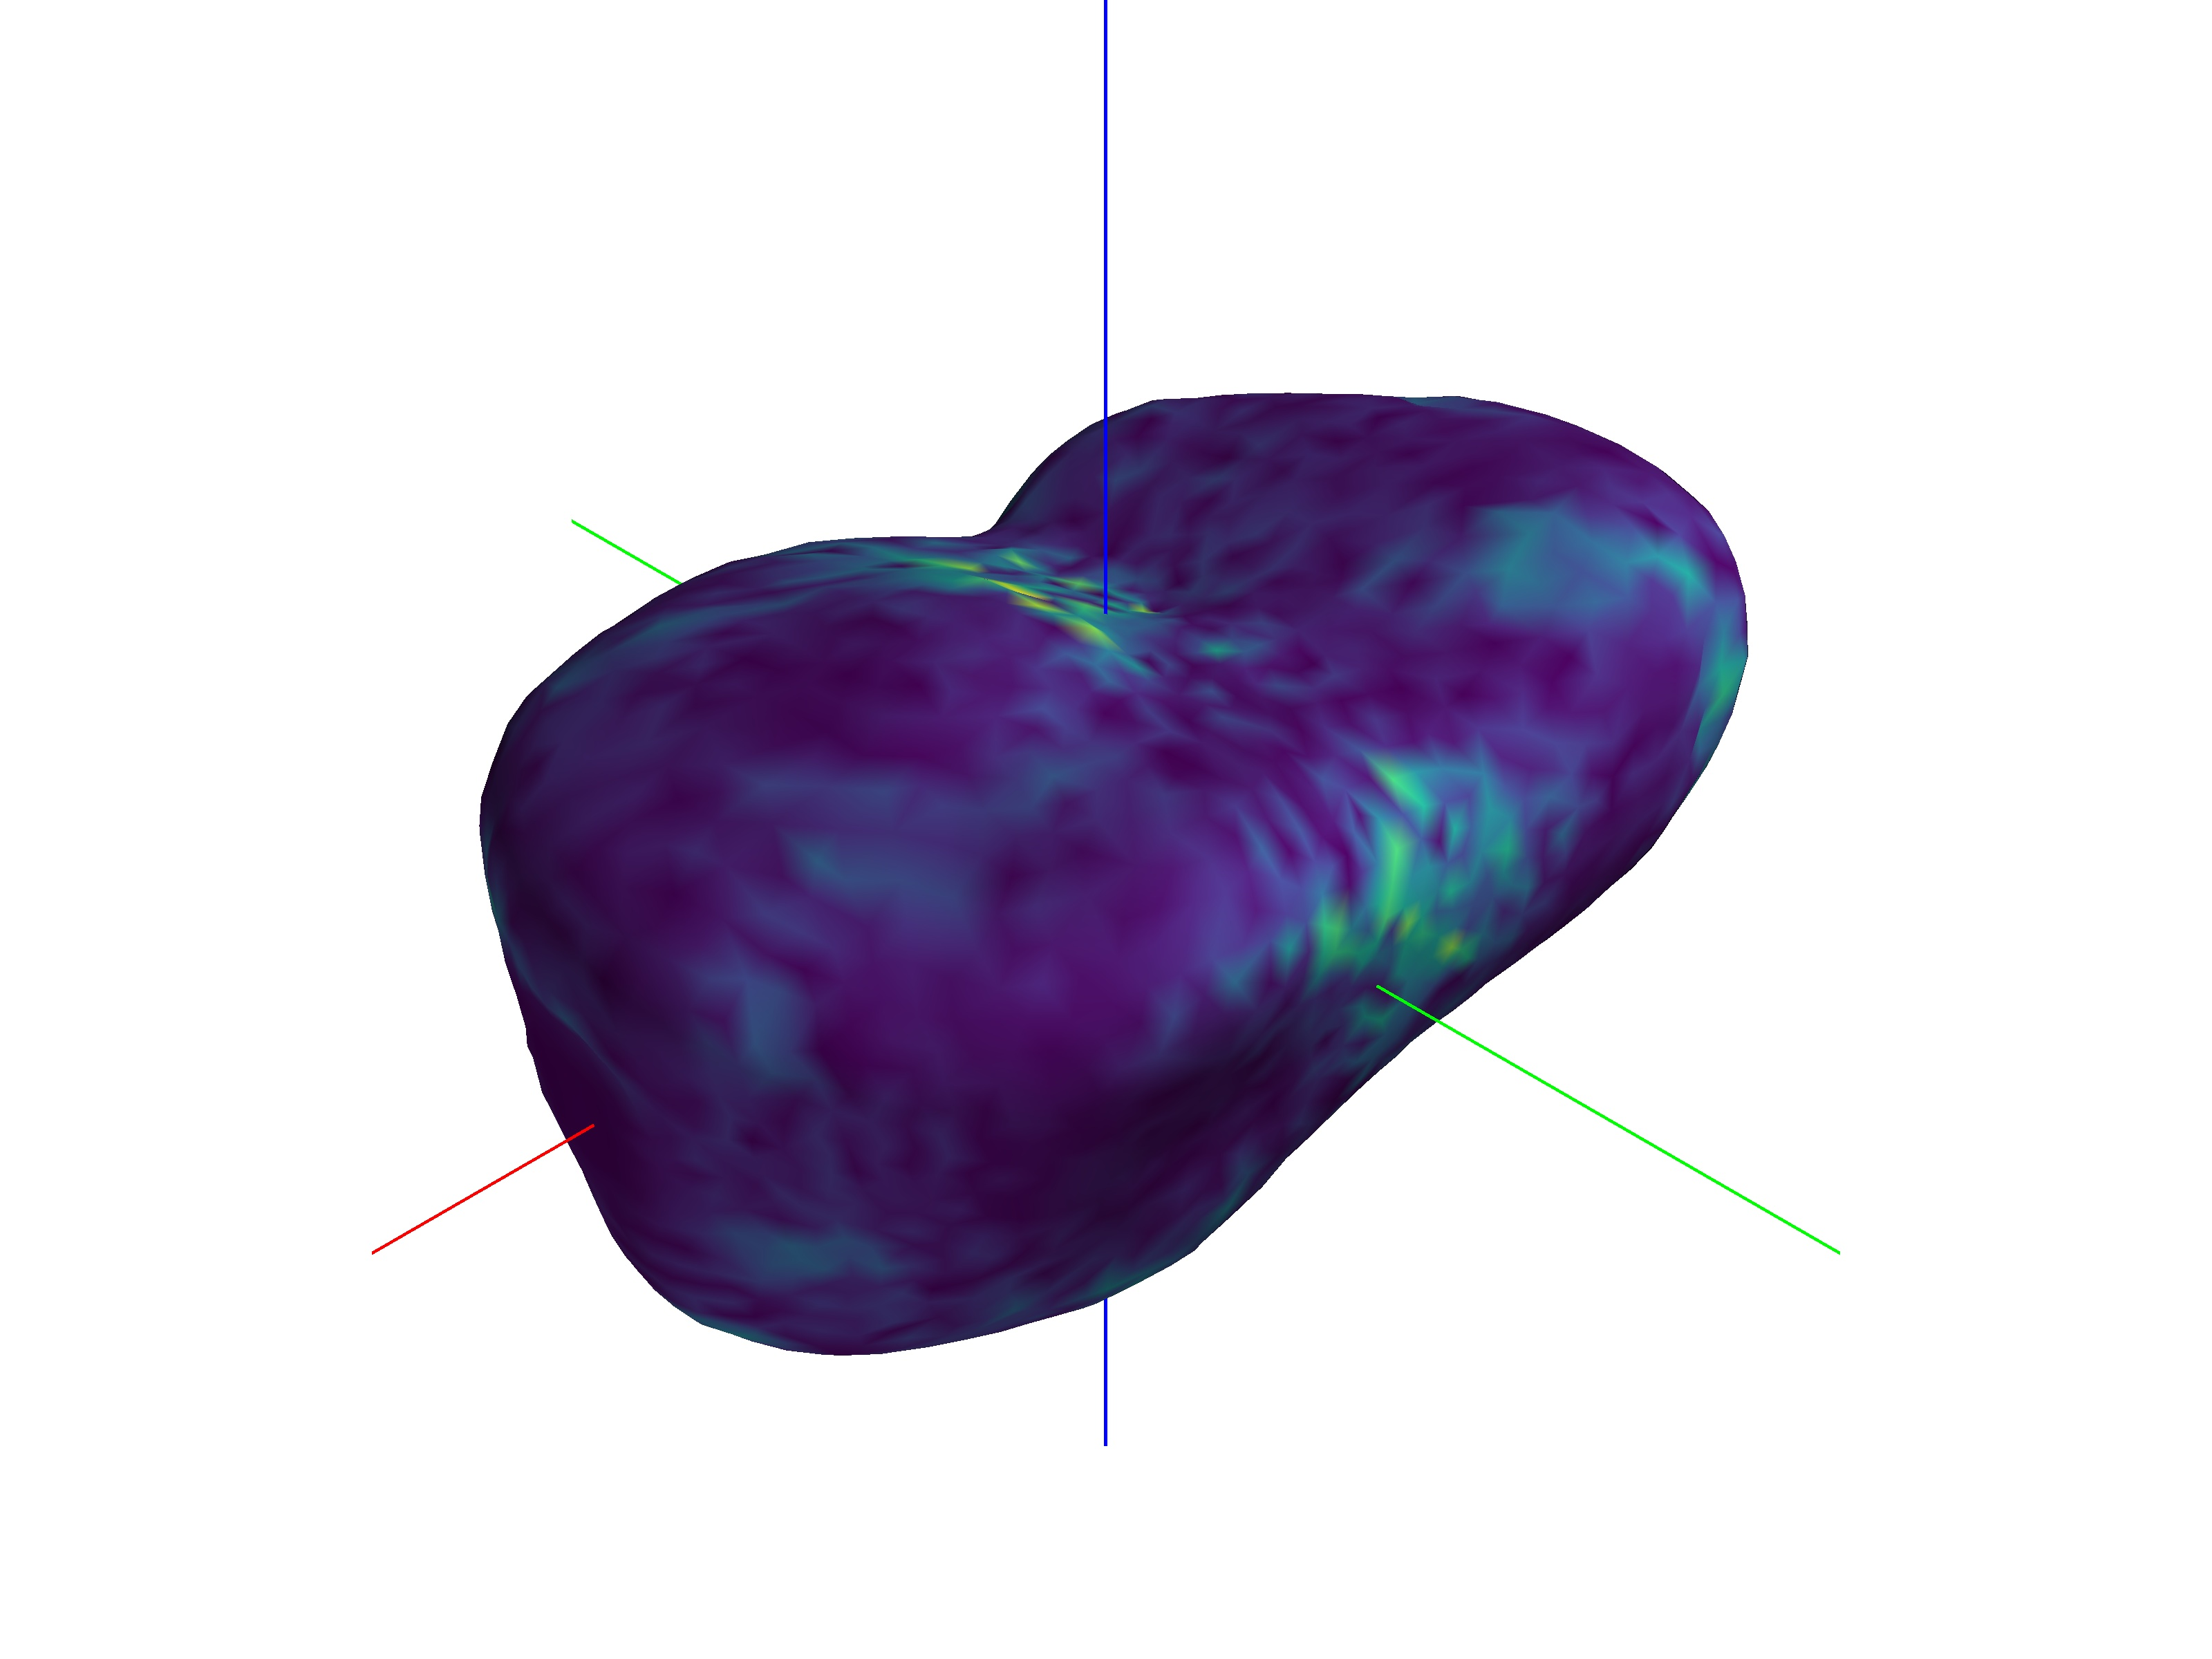
\includegraphics[trim={15cm 10cm 15cm 10cm},clip,height=0.5\textheight,width=0.3\textwidth,keepaspectratio]{figures/dynamic_exploration/castalia/partial_weights_11249.jpg}}%
    \subcaptionbox{\SI{100}{\percent} of measurements added\label{fig:castalia_partial_weights_100}}{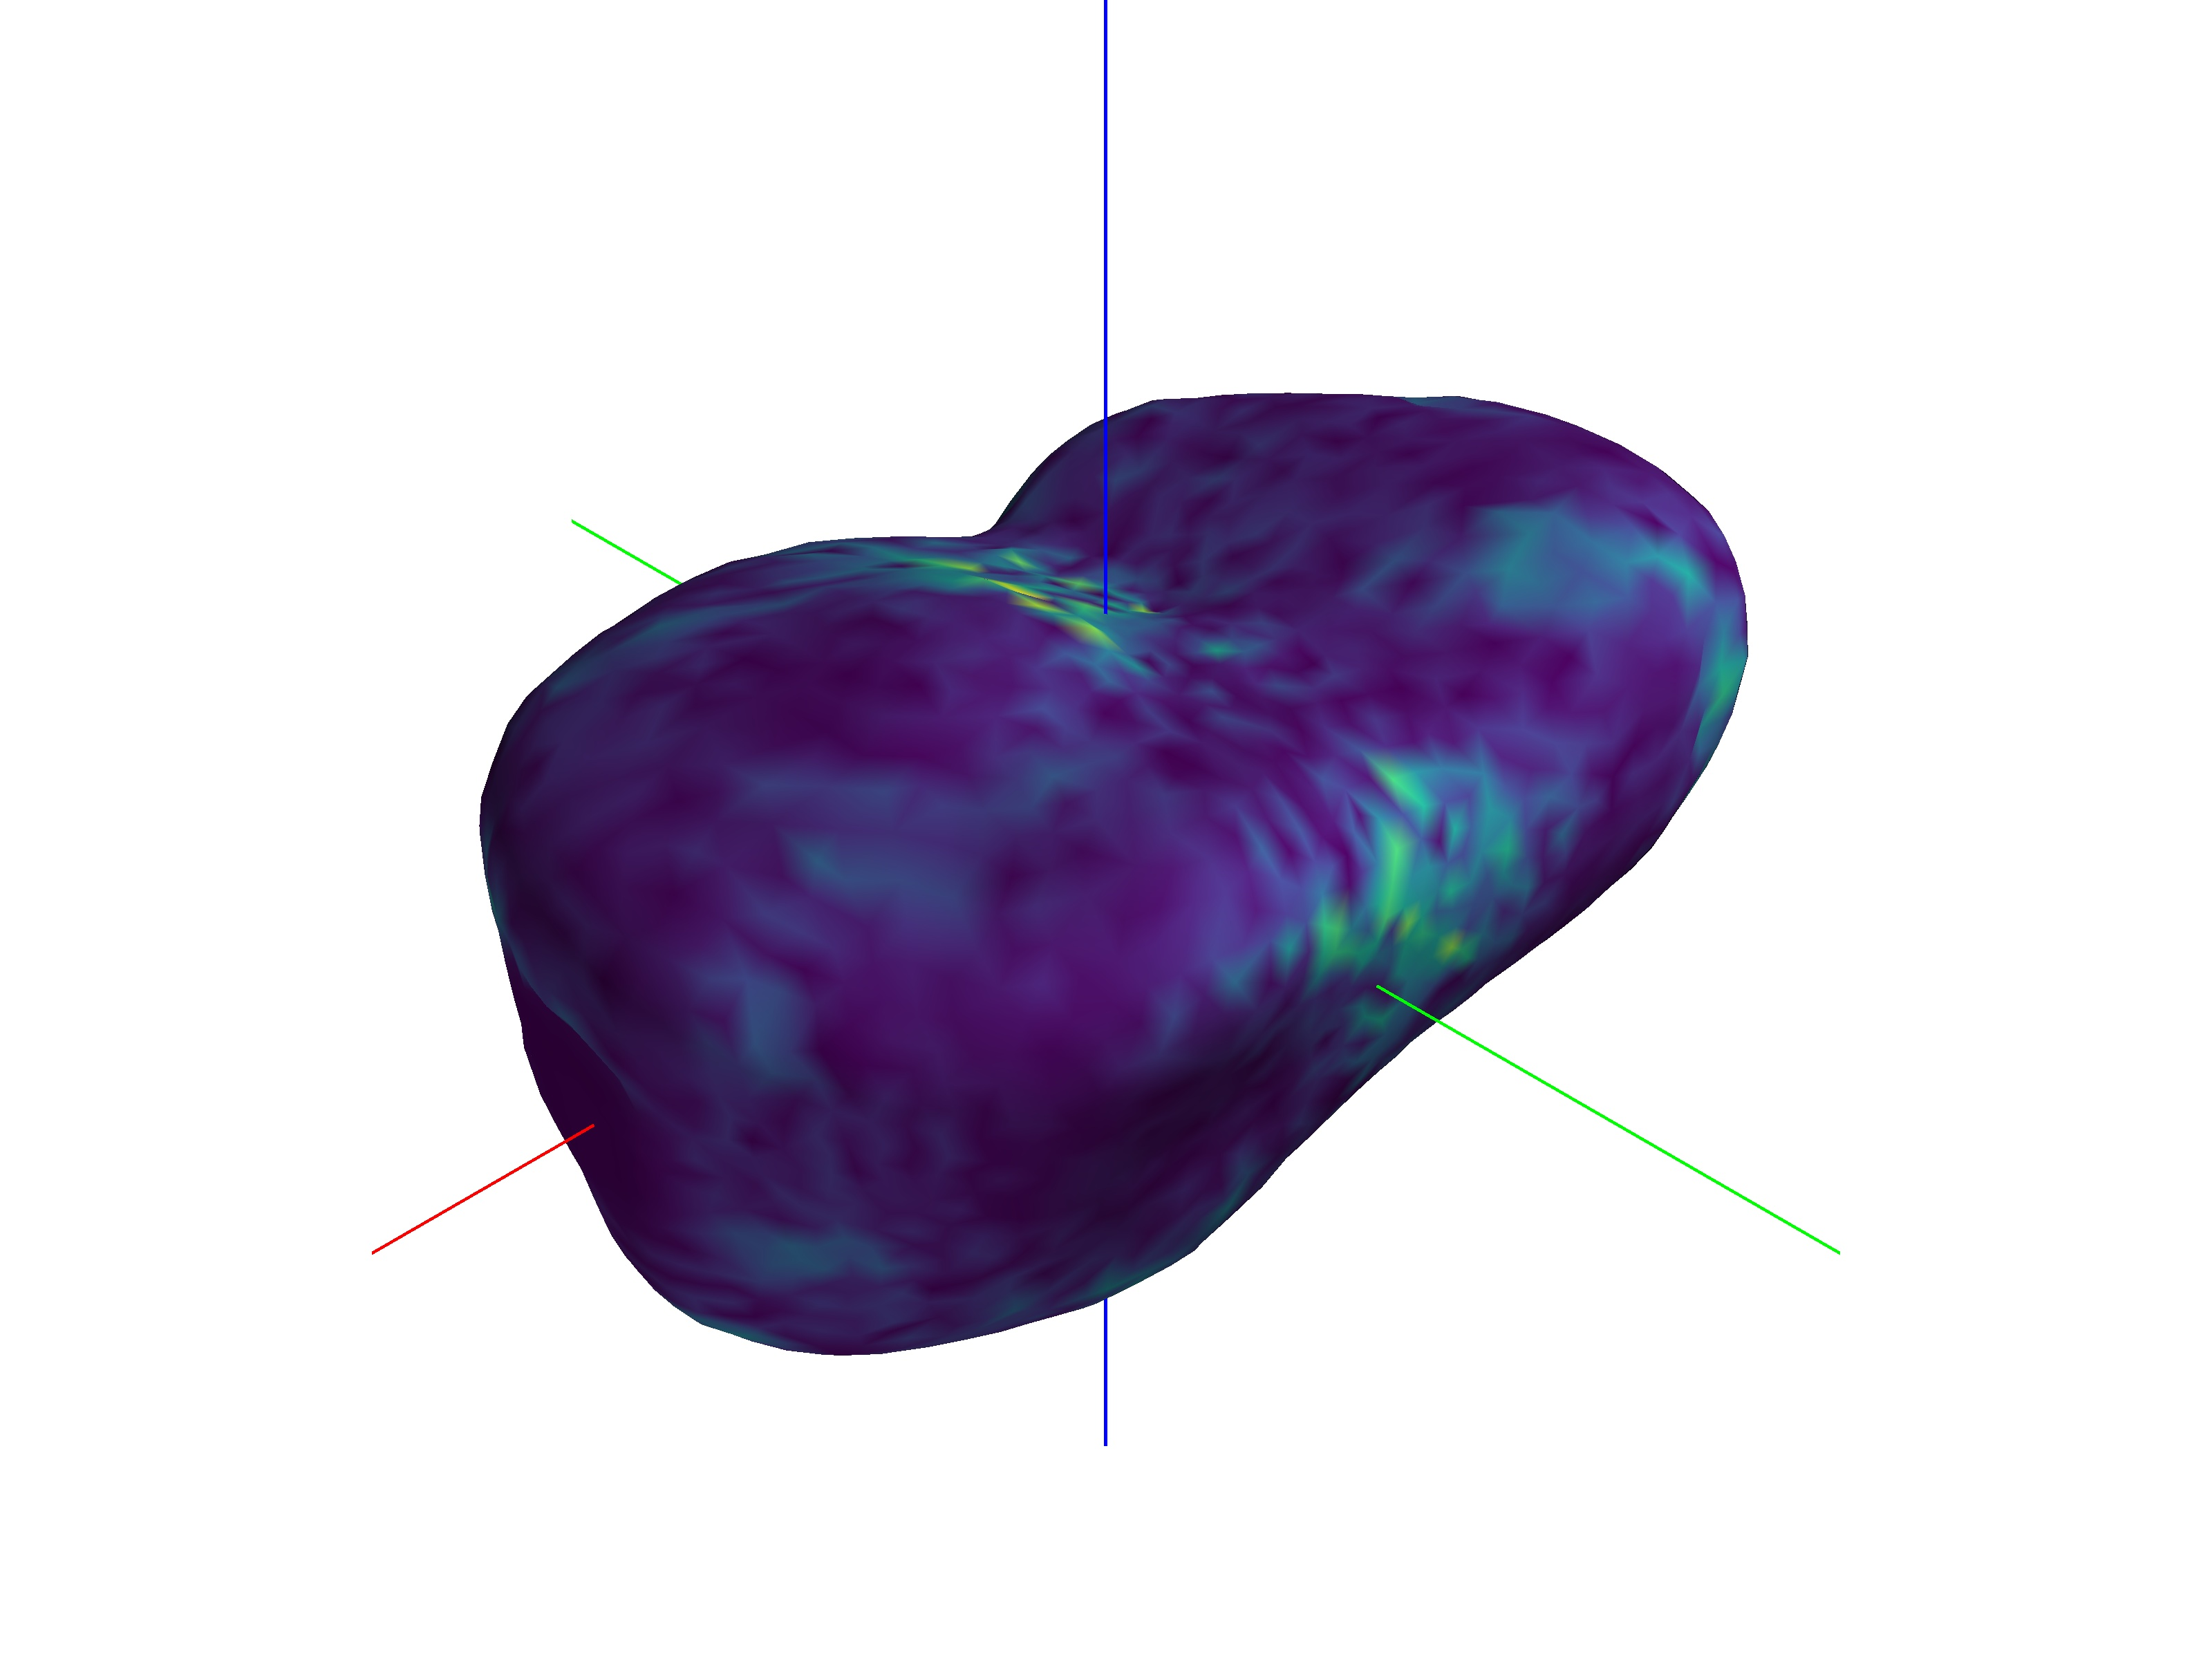
\includegraphics[trim={15cm 10cm 15cm 10cm},clip,height=0.5\textheight,width=0.3\textwidth,keepaspectratio]{figures/dynamic_exploration/castalia/partial_weights_14998.jpg}}%
    \subcaptionbox{True Shape Model\label{fig:castalia_weights_truth}}{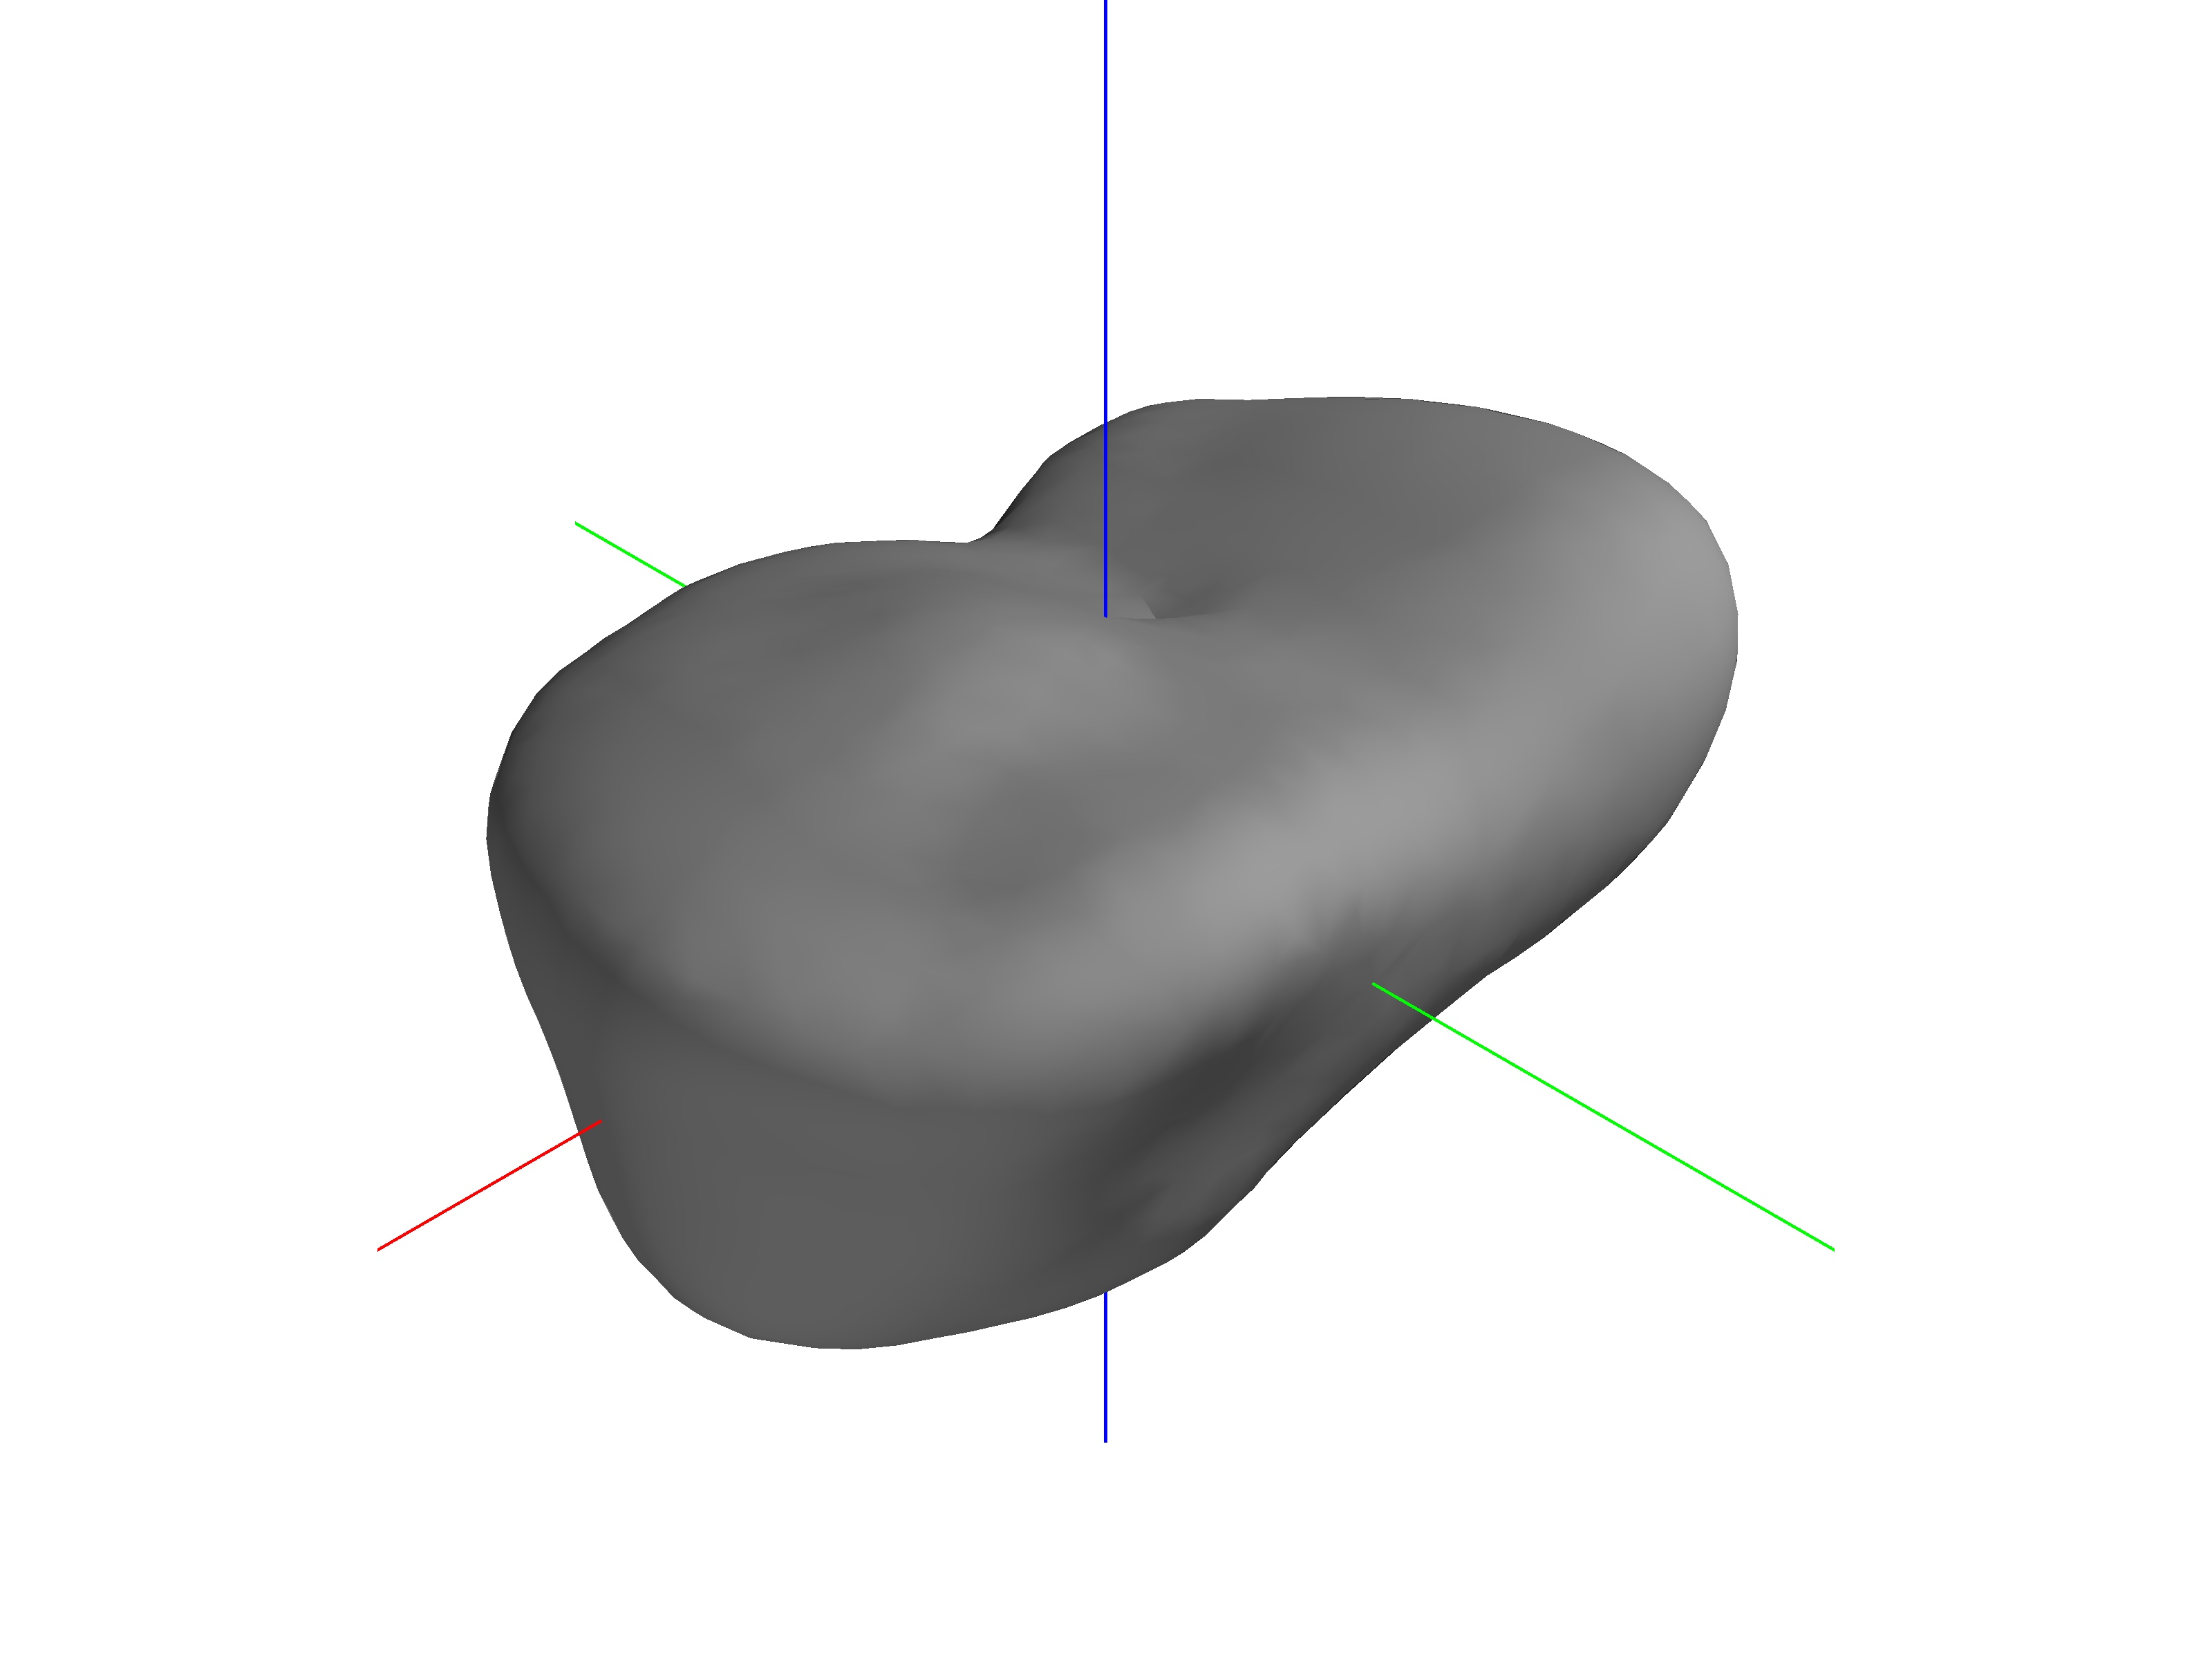
\includegraphics[trim={15cm 10cm 15cm 10cm},clip,height=0.5\textheight,width=0.3\textwidth,keepaspectratio]{figures/mesh_update/castalia/truth.jpg}}
    \caption[Asteroid Castalia shape reconstruction with uncertainty]{Incremental reconstruction of asteroid Castalia. The images colored according to the shape uncertainty. Areas of high uncertainty are in yellow while ares of low uncertainty are in purple.~\label{fig:castalia_weights_reconstruction}}
\end{figure}

\Cref{fig:castalia_metrics} shows the total normalized uncertainty and percent error for the volume estimate. 
The plots show that the reconstruction converges to an accurate shape estimate after approximately \SI{8000}{\second}.
In addition, the volume estimate is initially a much larger value but quickly converges to the true value.
\begin{figure}[htbp]
    \centering
    \tikzsetnextfilename{castalia_metrics}
\begin{tikzpicture}[baseline]
    \begin{groupplot}[
        group style={
            group name={castalia_metrics},
            group size=1 by 2,
            xlabels at=edge bottom,
            ylabels at=edge left,
            xticklabels at=edge bottom,
        },
        xlabel={Normalized Time},
        scale only axis,
        width=0.8\textwidth,
        height=0.1\textheight,
        ylabel style={align=center},
    ]
    \nextgroupplot[ylabel={Normalized\\Uncertainty}]
    \addplot [ultra thick, color=blue, mark=none] table [x=NORMALIZED_TIME, y=NORMALIZED_UNCERTAINTY, col sep=comma] {figures/dynamic_exploration/castalia/uncertainty.csv};
    \addplot [ultra thick,red, mark=none, dashed] coordinates {
        (0.0, 0.0) (1.0, 0.0) 
    };

    \nextgroupplot[ylabel={Volume Percent\\Error}]
    \addplot [ultra thick, blue, mark=none] table [x=NORMALIZED_TIME, y=VOLUME_PERCENT_ERROR, col sep=comma] {figures/dynamic_exploration/castalia/volume.csv};
        \addplot [ultra thick,red, mark=none, dashed] coordinates {
            (0.0, 0.0) (1.0, 0.0) 
        };
\end{groupplot}
\end{tikzpicture}


    \caption{Normalized uncertainty and volume percent error for Castalia\label{fig:castalia_metrics}}
\end{figure}
The spacecraft autonomously navigates around asteroid Castalia to best minimize the cost function in~\cref{eq:control_cost}.

% \paragraph{Castalia Landing Site Selection}

% With an appropriate shape estimate, the spacecraft can autonomously transition from a shape reconstruction to a landing mode.
% Based on the shape estimate we seek to determine the best location to land. 
% In reality, any landing site selection would be based on a wide variety of factors and constraints, however we highlight a few which can be determined autonomously and from the shape estimate.
% The first metric is related to the surface slope which is computed using the completed shape estimate and~\cref{eq:surface_slope}.
% Areas which violate the slope constraint of \( \phi < \SI{5}{\degree} \) are excluded from further consideration.
% \begin{figure}[htbp]
%     \centering
%     \subcaptionbox{Surface slope of Castalia\label{fig:surface_slope_castalia}}{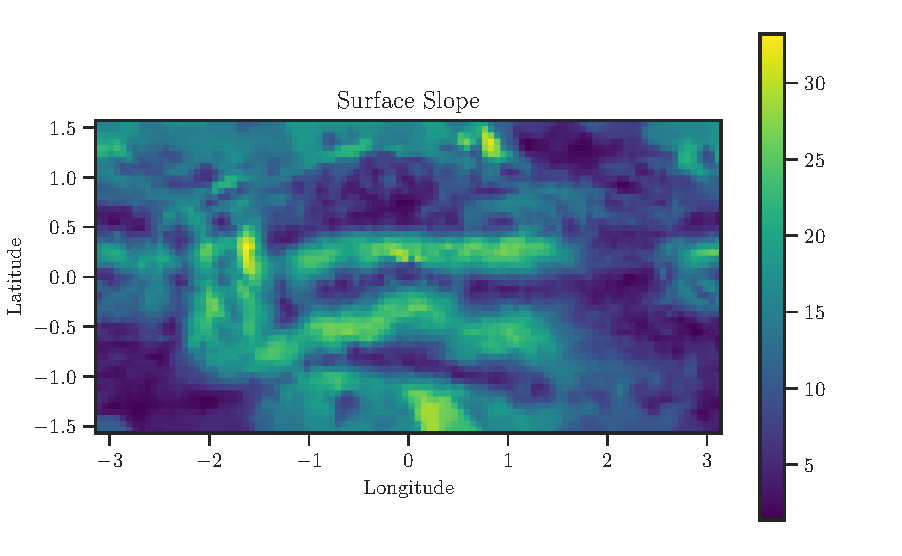
\includegraphics[width=0.5\textwidth]{figures/dynamic_exploration/castalia/refine/slope.pdf}}%
%     \subcaptionbox{Masked surface slope with areas \( \phi > \SI{5}{\degree}\) excluded\label{fig:surface_slope_castalia_masked}}{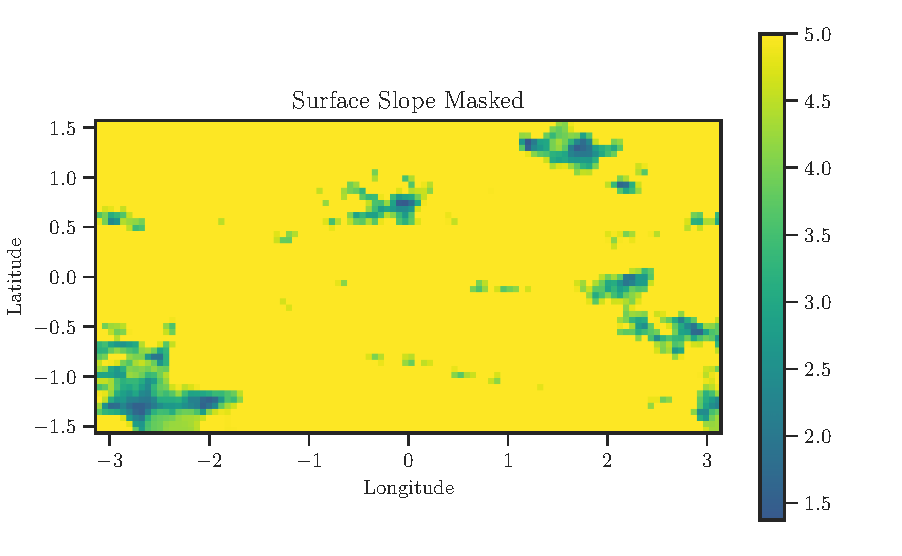
\includegraphics[width=0.5\textwidth,keepaspectratio]{figures/dynamic_exploration/castalia/refine/slope_masked.pdf}}
%     \caption{Surface slope of asteroid Castalia\label{fig:surface_slope_castalia_both}}
% \end{figure}

% The next metric is related to the distance from the current spacecraft position to all candidate landing sites on the surface.
% We utilize~\cref{eq:geodesic_distance} to compute a distance metric to the surface.
% Landing sites which are closer will be considered preferentially over those at a larger distance.
% \Cref{fig:distance_castalia_both} shows a surface plot of the distance to the surface. 
% The area immediately beneath the spacecraft has a small cost while those on the opposite side of the asteroid have a much larger cost.
% \begin{figure}[htbp]
%     \centering
%     \subcaptionbox{Surface Distance to surface of Castalia\label{fig:surface_distance_castalia}}{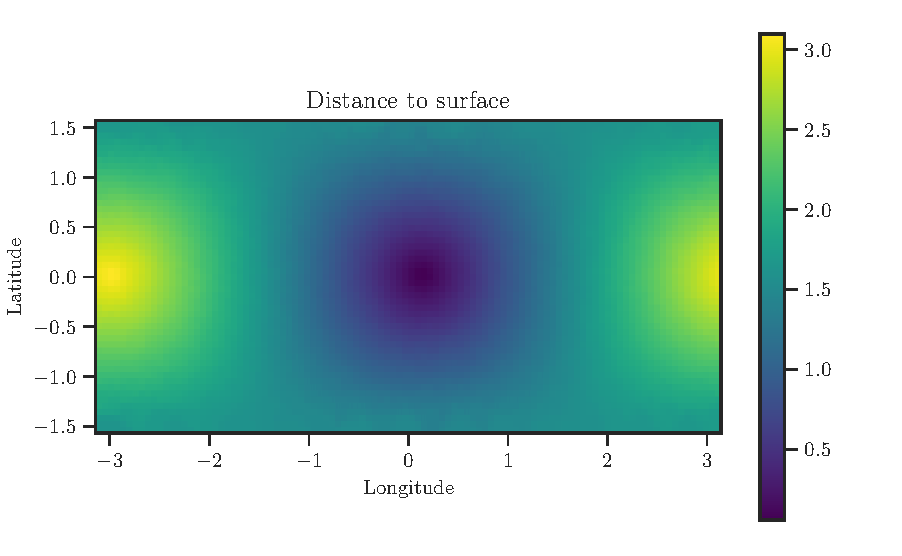
\includegraphics[width=0.5\textwidth]{figures/dynamic_exploration/castalia/refine/dist.pdf}}%
%     \subcaptionbox{Masked distance to surface with areas \( \phi > \SI{5}{\degree}\) excluded\label{fig:surface_distance_castalia_masked}}{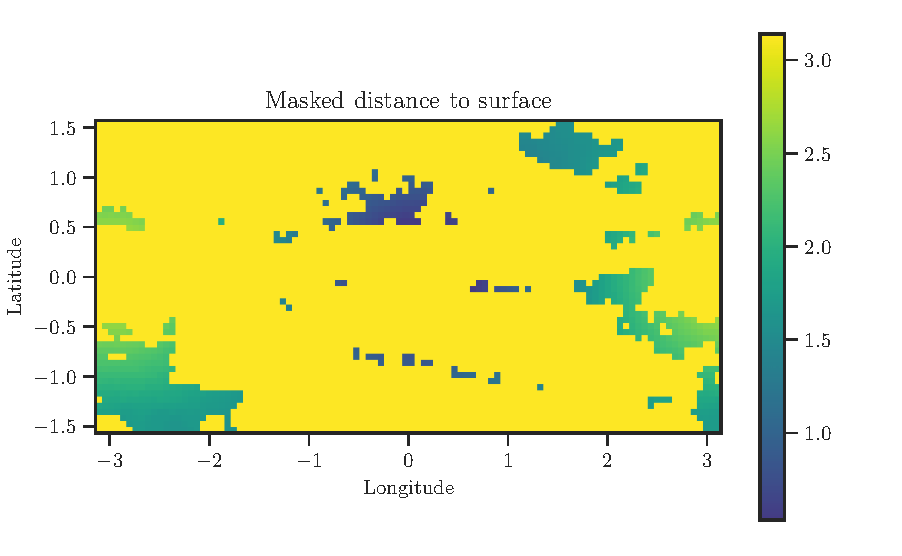
\includegraphics[width=0.5\textwidth,keepaspectratio]{figures/dynamic_exploration/castalia/refine/dist_masked.pdf}}
%     \caption{Distance to surface of asteroid Castalia\label{fig:distance_castalia_both}}
% \end{figure}
% We can combine~\cref{fig:distance_castalia_both,fig:surface_slope_castalia_both} to determine the best landing site. 
% The combination of the two is shown in~\cref{fig:landing_site_cost} with the desired landing site shown by the blue marker.
% \begin{figure}[htbp]
%     \centering
%     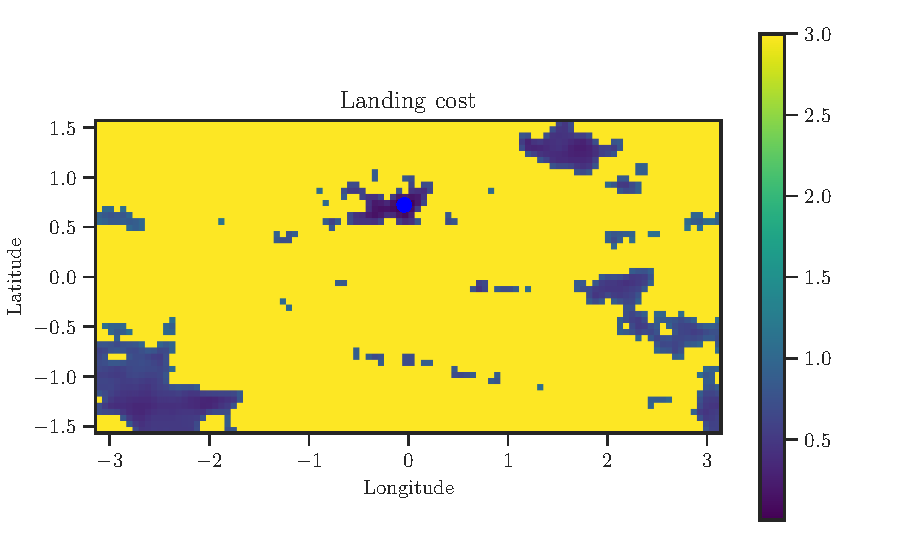
\includegraphics[width=0.75\textwidth,keepaspectratio]{figures/dynamic_exploration/castalia/refine/cost.pdf}
%     \caption{Total cost for surface landing based on surface slope and distance\label{fig:landing_site_cost}}
% \end{figure}
% After selecting the appropriate landing site we then prepare for landing by collecting more measurements in the region around the landing area.

% \paragraph{Castalia Landing Site Refinement}
% One key benefit of an in-situ spacecraft is the ability to measure surface features at a much higher resolution than is possible from the ground. 
% This detail provides a much higher fidelity data source than ground based measurements. 
% In order to emulate this in the simulation we augment the shape model of Castalia with several small craters and outcroppings as shown in~\cref{fig:castalia_refinement}.
% However, these small features would be difficult to capture with the current low resolution shape model of approximately \num{4000} faces.
% The lower number of faces is useful for the evaluation of the polyhedron potential model, it is not ideal for the capture of minute surface features. 
% As a result, we utilize the isotropic remeshing operation described previously to selectively increase the fidelity in the region about the desired landing site.
% \Cref{fig:castalia_refine_density} shows that the vertex density increases by approximately an order of magnitude in region immediately surround the landing site.
% \begin{figure}[htbp]
%     \centering
%     \subcaptionbox{Original vertex density of the initial shape estimate\label{fig:intial_vertex_density}}{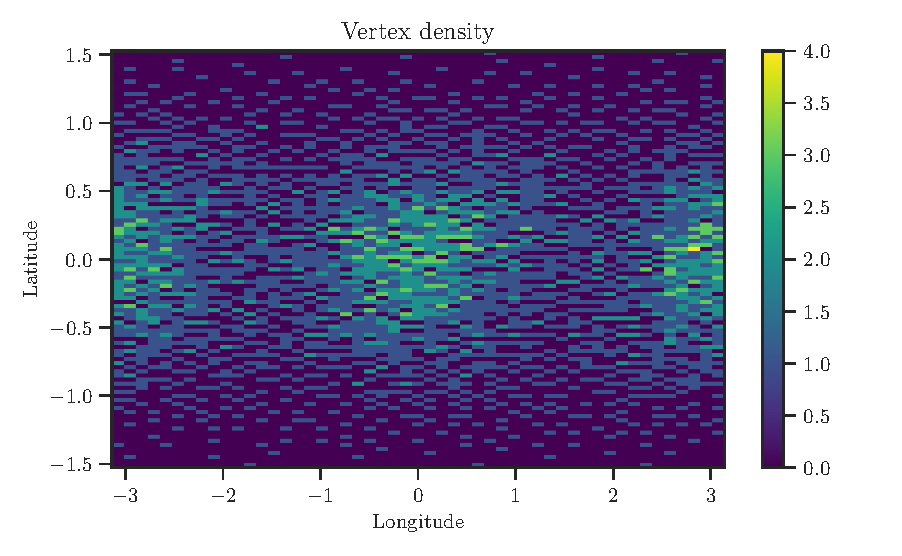
\includegraphics[width=0.5\textwidth]{figures/dynamic_exploration/castalia/refine/density.pdf}}%
%     \subcaptionbox{Vertex density after refinement  around landing site\label{fig:refine_vertex_density}}{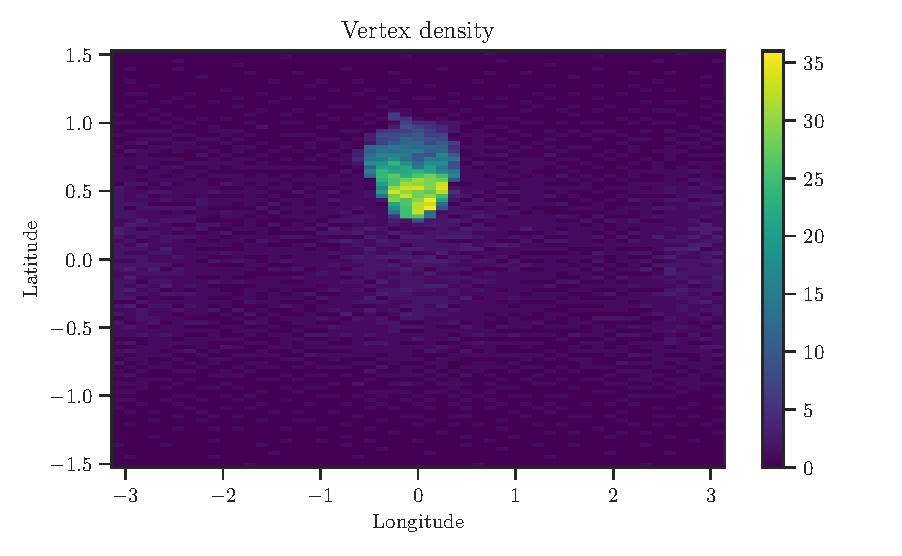
\includegraphics[width=0.5\textwidth]{figures/dynamic_exploration/castalia/land/density.pdf}}
%     \caption{Vertex density before and after refinement at asteroid Castalia\label{fig:castalia_refine_density}}
% \end{figure}

% The increased number of faces and vertices in the landing area allows for the capture of the small surface features.
% \Cref{fig:castalia_refinement} shows that given LIDAR measurements alone and the shape reconstruction algorithm that the small features are effectively estimated.
% \begin{figure}[htbp]
%     \centering
%     \subcaptionbox{Augmented shape of Castalia with surface features\label{fig:orig_castalia}}{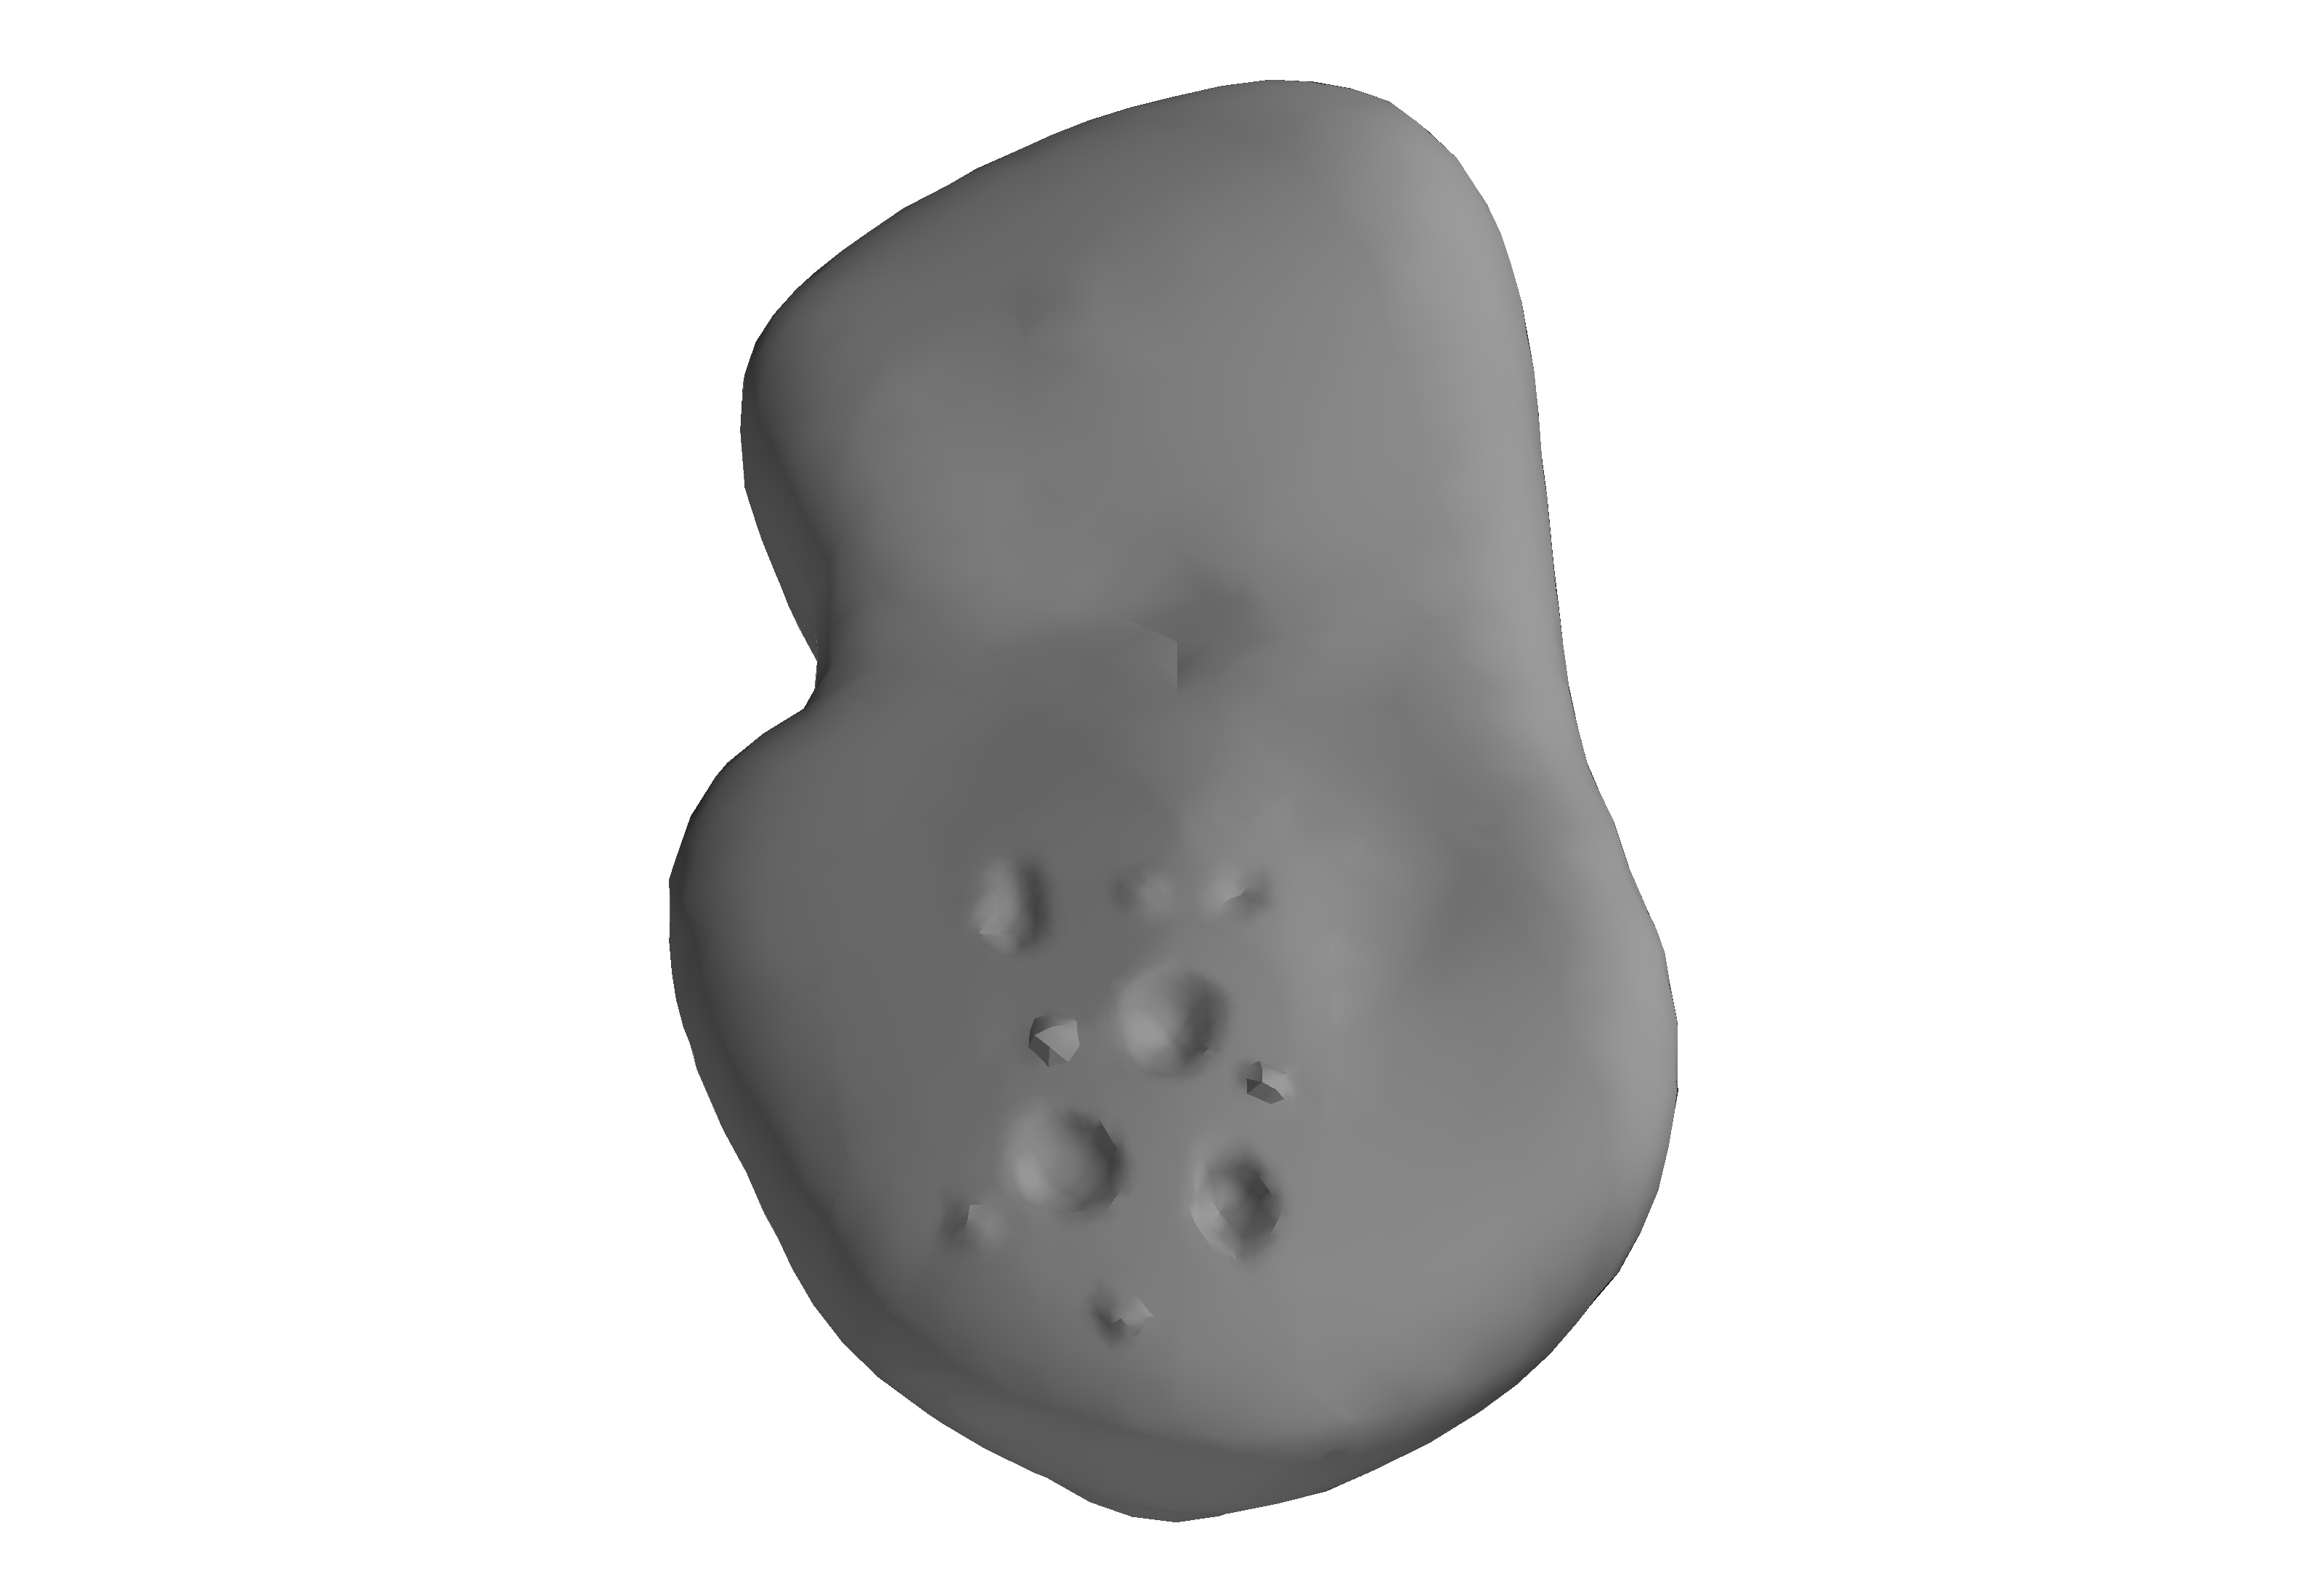
\includegraphics[trim={15cm 0 15cm 0},clip,keepaspectratio,height=0.2\textheight,width=0.5\textwidth]{figures/dynamic_exploration/castalia_bump_true.jpg}}%
%     \subcaptionbox{Estimated shape model after measuring the surface\label{fig:bump_castalia}}{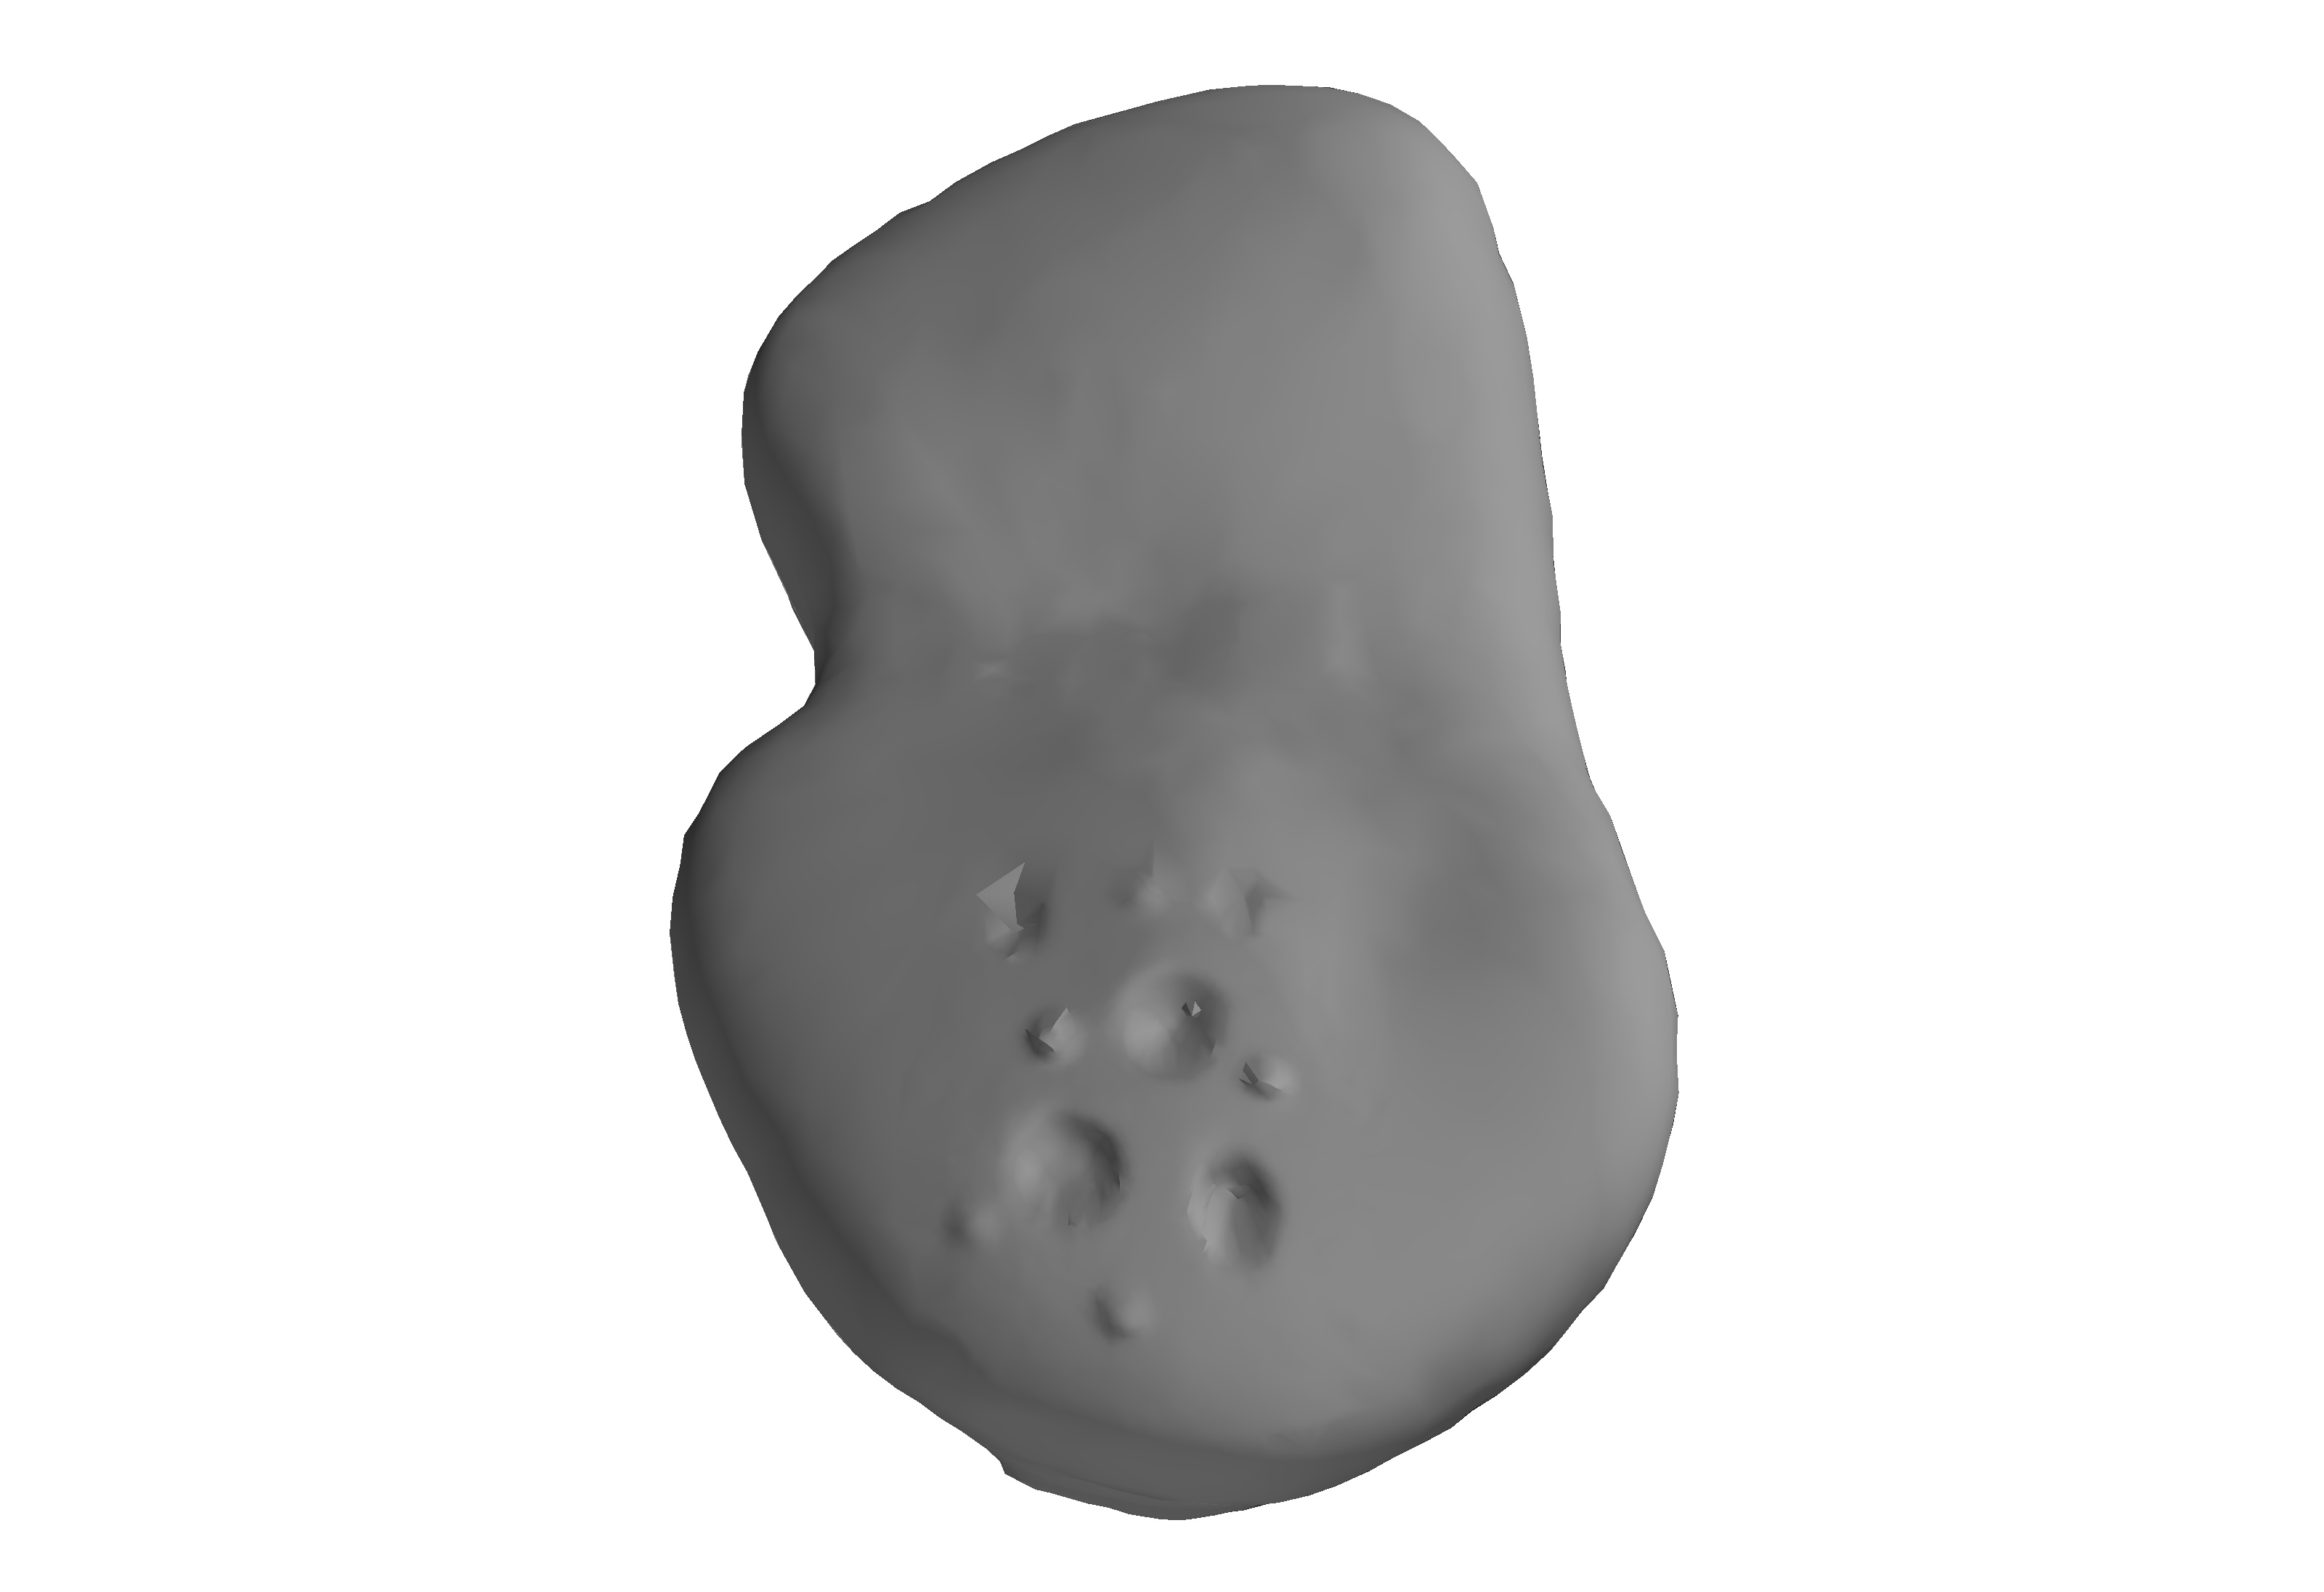
\includegraphics[trim={15cm 0 15cm 0},clip,keepaspectratio,height=0.2\textheight,width=0.5\textwidth]{figures/dynamic_exploration/castalia_bump_est.jpg}}
%     \caption{Asteroid Castalia with augmented with additional surface features~\label{fig:castalia_refinement}}
% \end{figure}

\paragraph{Castalia Vertical Descent}

The final phase of the simulation is to utilize the estimated shape model and vertically descend to the desired landing site. 
This is accomplished using the closed loop control of the vehicle and a trajectory which transitions from the home position to the surface over \SI{3600}{\second}.
The landing trajectory, using the estimated shape, is visualized in the asteroid frame in~\cref{fig:castalia_landing}.
During the vertical descent the vehicle is able to accurately track the desired trajectory using the estimated shape to compute the gravitational potential.
\begin{figure}[htbp]
    \centering
    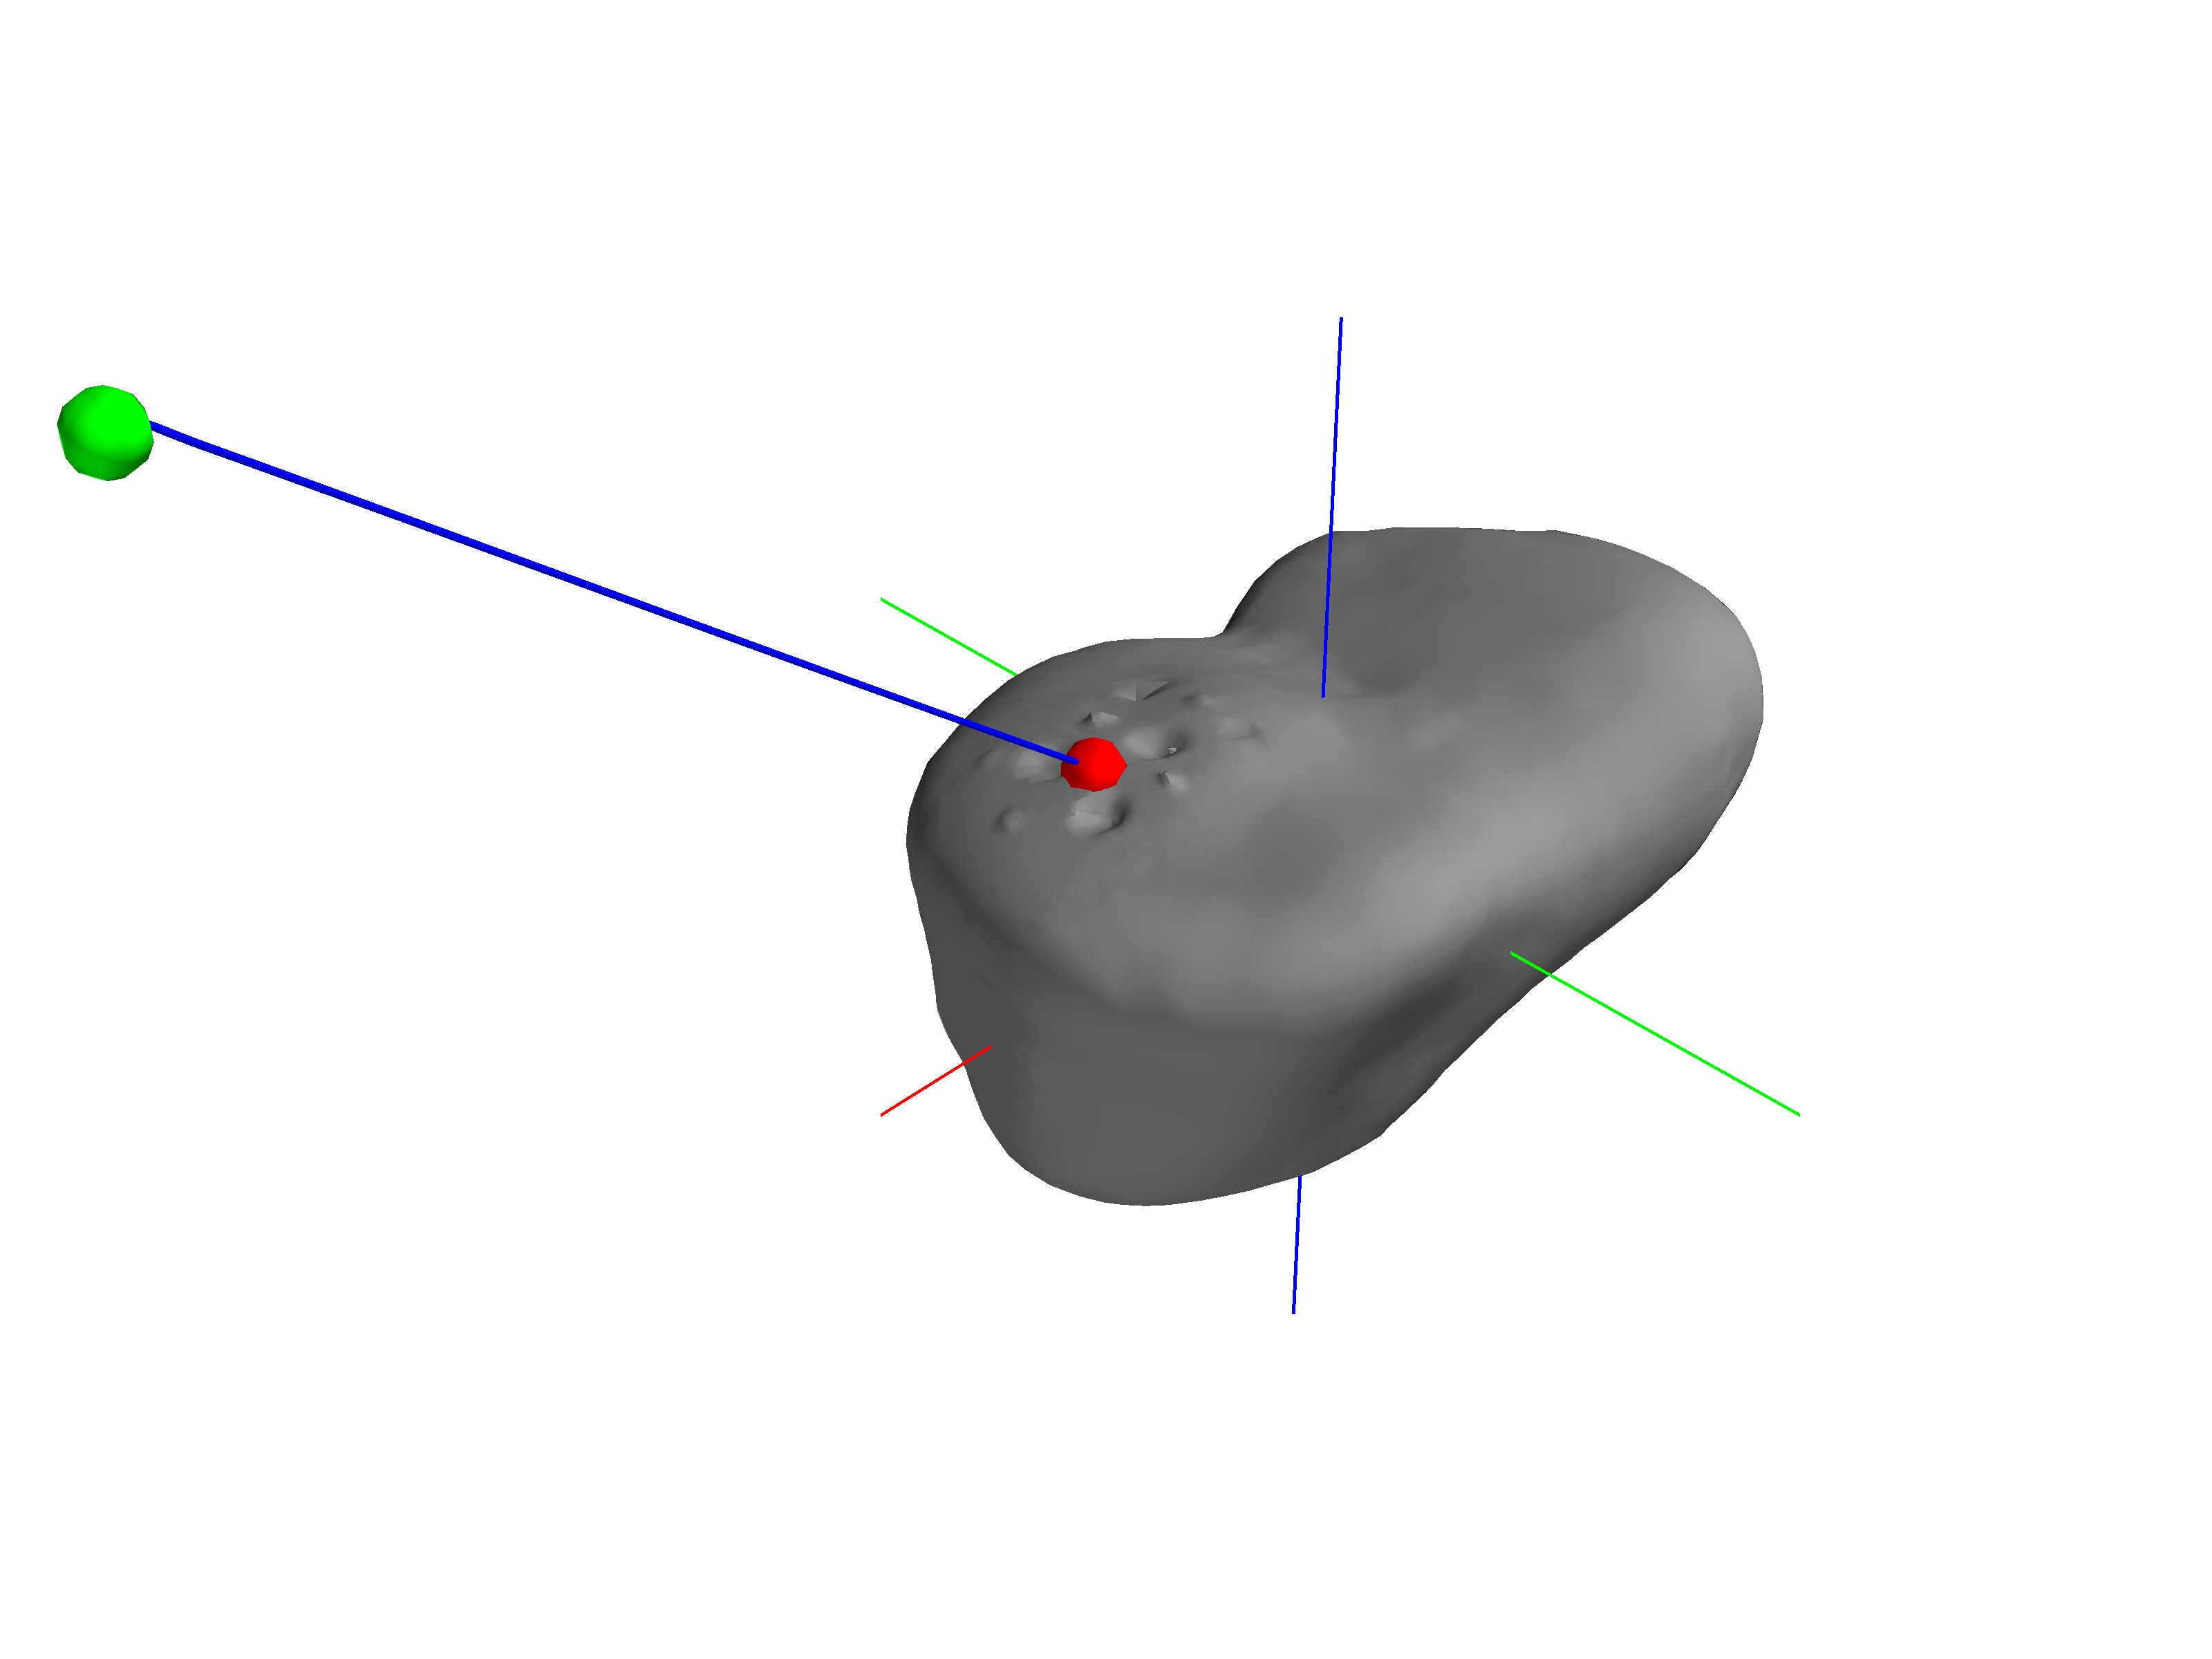
\includegraphics[width=0.5\textwidth]{figures/dynamic_exploration/castalia/land/asteroid_trajectory.jpg}
    \caption{Vertical descent onto 4769 Castalia~\label{fig:castalia_landing}}
\end{figure}

\section{Conclusions}

This paper developed a Bayesian update scheme to reconstruct the shape of a small body from range measurements. 
The approach allows for a local update operation that is able to reconstruct the shape in real time. 
This is in contrast to standard shape reconstruction algorithms which operate over the entire surface and require signification computational resources.
Next, an optimal guidance scheme is derived which determines the desired state to best update the shape estimate. 
This allows for a spacecraft to autonomously maneuver and reconstruct the shape of a small body without operator intervention.
% Finally, a mixed resolution shape representation is presented to allow for an increased fidelity in a specific region of the asteroid.
% This allows for a much greater shape accuracy in a local area while avoiding the computational costs associated with a uniformly high resolution mesh.
Several numerical examples were presented which demonstrates the approach on a number of real asteroids.







\section*{Appendix}

An Appendix, if needed, appears \textbf{before} research funding information and other acknowledgments.

\section*{Funding Sources}

Sponsorship information and acknowledgments of financial support should be included here. \textbf{Authors are responsible for accurately reporting funding data relevant to their research.} Please confirm that you have correctly entered \textbf{all sources} of funding and grant/award numbers \textbf{for all authors} in this section of your article. You will also be asked to select the appropriate funding organization from a drop-down menu in ScholarOne when you submit your manuscript. Be careful to choose the correct funder name, as organization names can be similar, and also be mindful to select sub-organizations within the registry hierarchy that are the actual funding sources, as appropriate, rather than choosing the name of the parent organization. Information provided in your manuscript must match the funding data entered in ScholarOne.

\section{Acknowledgement}
This research is supported in part by NSF under the grant CMMI-1335008.

\bibliography{library}


\end{document}
